% -*- LaTeX -*-
% -*- coding: utf-8 -*-
%
% ~~~~~~~~~~~~~~~~~~~~~~~~~~~~~~~~~~~~~~~~~~~~~~~~~~~~~~~~~~~~~~~~~~~~~~~~~~~~~~
%
%                             michael a.g. aïvázis
%                      california institute of technology
%                      (c) 1998-2010  all rights reserved
%
% ~~~~~~~~~~~~~~~~~~~~~~~~~~~~~~~~~~~~~~~~~~~~~~~~~~~~~~~~~~~~~~~~~~~~~~~~~~~~~~
%

\documentclass[10pt]{beamer}

% packages, setup, macros, etc.
% -*- LaTeX -*-
% -*- coding: utf-8 -*-
%
% ~~~~~~~~~~~~~~~~~~~~~~~~~~~~~~~~~~~~~~~~~~~~~~~~~~~~~~~~~~~~~~~~~~~~~~~~~~~~~~
%
%                             michael a.g. aïvázis
%                      california institute of technology
%                      (c) 1998-2010  all rights reserved
%
% ~~~~~~~~~~~~~~~~~~~~~~~~~~~~~~~~~~~~~~~~~~~~~~~~~~~~~~~~~~~~~~~~~~~~~~~~~~~~~~
%


% language
\usepackage[english]{babel}

% color
\usepackage{xcolor}

% fonts
\usepackage{amsfonts}
\usepackage{times}
%\usepackage[iso-8859-7]{inputenc}

% figures
\usepackage{graphicx}

% listings and their configurations
\usepackage[slide,algoruled,linesnumbered,noend]{algorithm2e}
\SetKwComment{tnm}{\#}{}
\SetKw{KwAnd}{and}
\SetKw{KwSend}{send}
\SetKw{KwRecv}{recv}
\SetKw{KwFrom}{from}

\usepackage{textcomp}
\usepackage{listings}
\definecolor{keywordcolor}{rgb}{.0,.0,1.0}
\definecolor{commentcolor}{gray}{.3}
\definecolor{stringcolor}{gray}{.0}
\definecolor{linenumbercolor}{gray}{.3}
\definecolor{listingbgcolor}{gray}{.97}

\definecolor{acm114@sand}{HTML}{dddbc5}
\definecolor{acm114@olive}{HTML}{474a41}
\definecolor{acm114@lava}{HTML}{413b38}

\lstnewenvironment{python}[2][]{
  \lstset{
    language=python,
    morekeywords={self,yield,False,True,None},
    %
    columns=flexible,
    upquote=true,
    %
    aboveskip=\bigskipamount,
    belowskip=\bigskipamount,
    %
    numbers=left,
    numberstyle=\color{linenumbercolor}\tiny,
    stepnumber=1,
    numbersep=5pt,
    numberblanklines=true,
    %
    basicstyle=\tt\scriptsize,
    keywordstyle=\color{keywordcolor},
    commentstyle=\color{commentcolor}\slshape,
    stringstyle=\color{stringcolor}\slshape,
    showstringspaces=false,
    %
    frame=tb,
    captionpos=t,
    backgroundcolor=\color{white},
    xleftmargin=.25in,
    xrightmargin=.1in,
    %
    escapeinside={\#@}{@},
    %
    #1
  }}{#2}

\lstnewenvironment{C}[1][]{
  \lstset{
    language=c,
    columns=flexible,
    upquote=true,
    %
    aboveskip=\bigskipamount,
    belowskip=\bigskipamount,
    %
    numbers=left,
    numberstyle=\color{linenumbercolor}\tiny,
    stepnumber=1,
    numbersep=5pt,
    numberblanklines=true,
    %
    basicstyle=\tt\scriptsize,
    keywordstyle=\color{blue},
    commentstyle=\color{commentcolor}\slshape,
    showstringspaces=false,
    %
    frame=tb,
    captionpos=t,
    backgroundcolor=\color{listingbgcolor},
    xleftmargin=.25in,
    xrightmargin=.1in,
    %
    escapeinside={//@}{@},
    %
    #1
  }}{}

% references
\usepackage[numbers]{natbib}
\bibliographystyle{unsrtnat}
\renewcommand\bibsection{\section{\refname}}
\def\newblock{\small}

% misc
\usepackage{dcolumn}
\newcolumntype{d}[1]{D{.}{.}{#1}}

\usepackage{url}
\usepackage{hyperref}


% shortcuts
\def\algref#1{{Alg.~\ref{alg:#1}}}
\def\alglineref#1{{line~\ref{line:#1}}}
\def\eqref#1{{Eq.~\ref{eq:#1}}}
\def\figref#1{{Fig.~\ref{fig:#1}}}
\def\secref#1{{Sec.~\ref{sec:#1}}}
\def\tabref#1{{Table~\ref{tab:#1}}}
\def\lstref#1{{Listing~\ref{lst:#1}}}
\def\lstlineref#1{{line~\ref{line:#1}}}

% macros
\def\bydef{\mathrel{\mathop:}=}
\def\CC{\mbox{\tt C}}
\def\GNU{\mbox{\tt GNU}}
\def\GSL{\mbox{\tt GSL}}
\def\RANLUX{\mbox{\tt RANLUX}}

\def\cpp{\mbox{\tt C++}}
%\def\cpp{\mbox{\tt C\raise.4ex\hbox{++}}}
\def\fortran{{\tt FORTRAN}}
\def\f90{{\tt FORTRAN90}}

\def\pyre{{\tt pyre}}

\def\order#1{\mbox{$\mathcal{O}(#1)$}}
\def\class#1{\mbox{\tt #1}}
\def\component#1{\mbox{\tt #1}}
\def\function#1{\mbox{\tt #1}}
\def\method#1{\mbox{\tt #1}}
\def\identifier#1{\mbox{\tt #1}}
\def\keyword#1{\mbox{\tt #1}}
\def\srcfile#1{\mbox{\tt #1}}

\def\insertionsort{\mbox{\sc Insertion-Sort}}
\def\mergesort{\mbox{\sc Merge-Sort}}
\def\merge{\mbox{\sc Merge}}

\def\TODO#1{{%
\subsubsection*{Still to do}%
\scriptsize\tt%
\begin{list}{\leftpointright}{} #1 \end{list}}}

% set up the PDF options
\hypersetup{
    pdftitle={ACM/CS 114: Winter 2010},
    pdfauthor={Michael A.G. A\"iv\'azis},
    pdfsubject={Lecture notes},
    pdfkeywords=,           % list of keywords
%
    bookmarks=true,         % show bookmarks bar?
    unicode=false,          % non-Latin characters in Acrobat's bookmarks
    pdftoolbar=true,        % show Acrobat's toolbar?
    pdfmenubar=true,        % show Acrobat's menu?
    pdffitwindow=true,      % page fit to window when opened
    pdfnewwindow=true,      % links in new window
    colorlinks=true,        % false: boxed links; true: colored links
    linkcolor=acm114@sand,  % color of internal links
    citecolor=acm114@sand,  % color of links to bibliography
    filecolor=acm114@sand,  % color of file links
    urlcolor=acm114@sand    % color of external links
}
% end of file 


% the document
\title[ACM/CS 114 -- Winter 2010]{ACM/CS 114 \\ Parallel algorithms for scientific applications}
\author{Michael A.~G.~A\"iv\'azis}
\institute{California Institute of Technology}
\date{Winter 2010}

\begin{document}

% title slide
\begin{frame}
  \titlepage
\end{frame}

% what to build
%\includeonlylecture{20100106}
%\includeonlylecture{20100108}
%\includeonlylecture{20100111}

% lectures
% -*- LaTeX -*-
% -*- coding: utf-8 -*-
%
% ~~~~~~~~~~~~~~~~~~~~~~~~~~~~~~~~~~~~~~~~~~~~~~~~~~~~~~~~~~~~~~~~~~~~~~~~~~~~~~
%
%                             michael a.g. aïvázis
%                      california institute of technology
%                      (c) 1998-2010  all rights reserved
%
% ~~~~~~~~~~~~~~~~~~~~~~~~~~~~~~~~~~~~~~~~~~~~~~~~~~~~~~~~~~~~~~~~~~~~~~~~~~~~~~
%

\lecture{Organizational meeting}{20100104}


% end of file 

% -*- LaTeX -*-
% -*- coding: utf-8 -*-
%
% ~~~~~~~~~~~~~~~~~~~~~~~~~~~~~~~~~~~~~~~~~~~~~~~~~~~~~~~~~~~~~~~~~~~~~~~~~~~~~~
%
%                             michael a.g. aïvázis
%                      california institute of technology
%                      (c) 1998-2010  all rights reserved
%
% ~~~~~~~~~~~~~~~~~~~~~~~~~~~~~~~~~~~~~~~~~~~~~~~~~~~~~~~~~~~~~~~~~~~~~~~~~~~~~~
%

\lecture{Introduction to scientific computing}{20100106}


\begin{frame}

  \begin{itemize}
                        
  \end{itemize}

\end{frame}

% end of file 

% -*- LaTeX -*-
% -*- coding: utf-8 -*-
%
% ~~~~~~~~~~~~~~~~~~~~~~~~~~~~~~~~~~~~~~~~~~~~~~~~~~~~~~~~~~~~~~~~~~~~~~~~~~~~~~
%
%                             michael a.g. aïvázis
%                      california institute of technology
%                      (c) 1998-2010  all rights reserved
%
% ~~~~~~~~~~~~~~~~~~~~~~~~~~~~~~~~~~~~~~~~~~~~~~~~~~~~~~~~~~~~~~~~~~~~~~~~~~~~~~
%

\lecture{Overview of parallel systems}{20100108}

% --------------------------------------
% motivation for parallel computing
\begin{frame}[fragile]
%
  \frametitle{Motivations for going parallel}
%
  \begin{itemize}
%
  \item why bother?
    \begin{itemize}
    \item {\em speed}: there are fundamental limits to the processing power of a single processor
    \item {\em throughput}: time to solution is critical for many problems
    \item {\em size}: high resolution requires lots of memory
    \item {\em availability}: the tool exists, use it
    \end{itemize}
%
  \item but, be careful
    \begin{itemize}
    \item the commercial market is unstable
    \item the computing environment is somewhat primitive
    \item software packages and libraries are emerging slowly
    \item parallel programming is not hard, but it requires {\em discipline}
    \end{itemize}
%
  \end{itemize}
%
\end{frame}

% --------------------------------------
% computer system taxonomy
\begin{frame}[fragile]
%
  \frametitle{Taxonomy}
%
  \begin{itemize}
%
  \item an early classification of computer systems focused on the relation between {\em
    instruction streams} and {\em data streams}:
    \begin{itemize}
      \item SISD: single instruction, single data
      \item: SIMD: single instruction, multiple data
      \item: MIMD: multiple instruction, multiple data
    \end{itemize}
%
    \item SISD describes conventional serial computers
    \begin{itemize}
      \item the programming model; the hardware has moved on...
    \end{itemize}
%
    \item SIMD and MIMD are the traditional models for parallel machines
%
    \item MIMD systems are often programmed in SPMD mode: single {\em program}, multiple data
  \end{itemize}
%
\end{frame}

% --------------------------------------
% architectural issues
\begin{frame}[fragile]
%
  \frametitle{Architectural issues}
%
  \begin{itemize}
%
  \item {\em control:} SIMD vs.~MIMD
  \item {\em co\"ordination}: synchronous vs.~asynchronous
  \item {\em memory organization}: private vs.~shared
  \item {\em address space}: local vs.~global
  \item {\em memory access}: uniform vs.~ non-uniform
  \item {\em granularity}: the power of each processor
  \item {\em scalability}: dependence on the number of processors
  \item {\em interconnect}: topology, routing, switching
%
  \end{itemize}
%
\end{frame}

% --------------------------------------
% tradeoffs
\begin{frame}[fragile]
%
  \frametitle{Tradeoffs}
%
  \begin{center}
    \begin{minipage}{.75\linewidth}
      \begin{tabular}{l|l|l}
                        & shared memory & distributed memory \\ \hline
        scalability     & {\em harder}  & {\em easier} \\
        programmability & {\em easier}  & {\em harder}
      \end{tabular}
    \end{minipage}
  \end{center}

%
  \begin{itemize}
%
  \item shared memory permits parallelizing serial program gradually, focusing on worst
    bottlenecks first
%
  \item distributed memory requires partitioning and distributing both data and work across
    processors, which usually rules out incremental parallelization
%
  \end{itemize}
%
\end{frame}

% --------------------------------------
% categories of parallel architectures
\begin{frame}[fragile]
%
  \frametitle{Categories of parallel architectures}
%
  \begin{itemize}
%
  \item vector or array processor
  \item SMP: symmetric multiprocessor
  \item MPP: massively parallel multiprocessor
  \item DSM: distributed shared memory
  \item clusters
  \item hybrids
    \begin{itemize}
      \item SMP or MPP with vector processors
      \item networked clusters of SMPs
      \item SMP+GPGPU 
    \end{itemize}
%
  \end{itemize}
%
\end{frame}

% --------------------------------------
% memory hierarchy
\begin{frame}[fragile]
%
  \frametitle{Memory hierarchy}
%
  \begin{itemize}
  \item High performance architectures have a multi-tier memory hierarchy
%
    \begin{itemize}
%
    \item registers
    \item on-chip caches, usually referred to as level 1
    \item off-chip caches (level 2)
    \item random access memory
    \item remote memory (off processor)
    \item virtual memory, known as paging memory, that usually involves secondary storage
    \item secondary storage (disks)
    \item tertiary storage (tapes)
%
    \end{itemize}
%
  \end{itemize}
%
\end{frame}

% --------------------------------------
% parallel programming paradigms
\begin{frame}[fragile]
%
  \frametitle{Parallel programming paradigms}
%
  \begin{itemize}
%
  \item {\em functional languages}: specify what to compute, not how
  \item {\em parallelizing compilers}: automatic or semi-automatic detection of parallelism in
    serial code; mostly loop-unrolling, often with the help of special mark up (pragmas)
  \item {\em object oriented}: parallelism encapsulated within distributed objects

  \item {\em data parallel}: simultaneous operations on memory; mostly arrays
  \item {\em shared memory}: multiple threads executing a pool of tasks using common memory
  \item {\em remote memory access}: one sided put/get communication between processes
  \item {\em message passing}: two sided, co\"ordinated send/receive communication between
    processes
%
  \end{itemize}
%
\end{frame}

% --------------------------------------
% designing parallel algorithms
\begin{frame}[fragile]
%
  \frametitle{Designing parallel algorithms}
%
  \begin{itemize}
%
  \item {\em identification}: identify the part of the problem that can be parallelized
  \item {\em partition}: decompose the parallelizable part into fine-grained tasks
  \item {\em communication}: determine the necessary communication patterns among tasks
  \item {\em coarsening}: combine into coarser tasks and adjust the communication patterns
  \item {\em task mapping}: assign tasks to processors
%
  \end{itemize}
%
\end{frame}

% --------------------------------------
% paradigms for parallel algorithms
\begin{frame}[fragile]
%
  \frametitle{Paradigms for parallel algorithms}
%
  \begin{itemize}
%
  \item {\em embarrassingly parallel}: mostly independent tasks
  \item {\em functional decomposition}: based on computation
  \item {\em domain decomposition}: based on data
  \item {\em data parallel}: array operations
  \item {\em divide-and-conquer}: tree-like partitioning
  \item {\em pipelining}: overlapping stages
%
  \end{itemize}
%
\end{frame}

% --------------------------------------
% template
\begin{frame}[fragile]
%
  \frametitle{Blank}
%
  \begin{itemize}
%
  \item a point
%
  \end{itemize}
%
\end{frame}

% end of file 

% -*- LaTeX -*-
% -*- coding: utf-8 -*-
%
% ~~~~~~~~~~~~~~~~~~~~~~~~~~~~~~~~~~~~~~~~~~~~~~~~~~~~~~~~~~~~~~~~~~~~~~~~~~~~~~
%
%                             michael a.g. aïvázis
%                      california institute of technology
%                      (c) 1998-2010  all rights reserved
%
% ~~~~~~~~~~~~~~~~~~~~~~~~~~~~~~~~~~~~~~~~~~~~~~~~~~~~~~~~~~~~~~~~~~~~~~~~~~~~~~
%

\lecture{Introduction to parallel programming models}{20100111}

% --------------------------------------
% generic parallel architecture
\begin{frame}[fragile]
%
  \frametitle{Impact of architecture on algorithm design}
%
  \begin{itemize}
%
    \item recall the five steps of parallel algorithm design
      \begin{itemize}
      \item identification of the parallelizable part, partitioning into fine grain tasks,
        examination of the task communication patterns, task coarsening, and mapping coarse
        tasks onto processors
      \end{itemize}
%
    \item and the layout of the generic parallel architecture:
%
  \begin{figure}
    \centering
    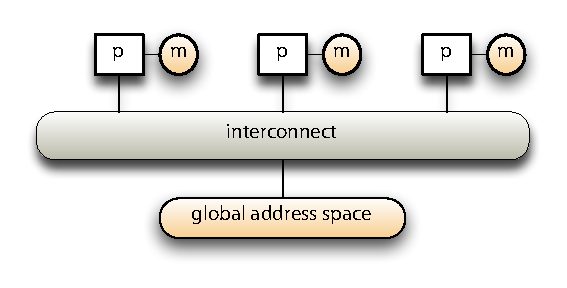
\includegraphics[width=.70\linewidth]{figures/generic-parallel-architecture.pdf}
    \label{fig:gpa-redux}
  \end{figure}
%
  \item let's move memory around and examine how this affects the programming model
  \item for a trivial but instructive problem
  \end{itemize}
%
\end{frame}

% --------------------------------------
% template
\begin{frame}[fragile]
%
  \frametitle{Parallel programming models}
%
  \begin{itemize}
%
  \item control
    \begin{itemize}
    \item how is parallelism {\em created}
    \item what is the {\em sequencing} of instruction streams in each task
    \item how do tasks {\em synchronize}
    \end{itemize}
%
    \item data address spaces
      \begin{itemize}
        \item what data is private to each task; what data must be shared
        \item how is logically shared data created, accessed or communicated, and synchronized
      \end{itemize}
%
    \item instruction sets
      \begin{itemize}
      \item what are the fundamental operations for process creation, communication,
        and synchronization
      \item which operations are {\em atomic}
      \end{itemize}
%
    \item cost
      \begin{itemize}
      \item how fast does it run
      \item are resources used efficiently
      \item how hard is it to code correctly
      \end{itemize}
%
  \end{itemize}
%
\end{frame}

% --------------------------------------
% problem setup
\begin{frame}[fragile]
%
  \frametitle{Embarrassingly parallel: $p$ processor reduction}
%
  \begin{itemize}
%
  \item given a function $f$ and a sequence of numbers $S$ of length $N$, evaluate the sum
    \[
    s = \sum_{i=0}^{N-1}f(S_{i})
    \]
%
  \item parallel tasks: the function evaluations, the computation of partial sums
%
  \item strategy: assign $n/p$ numbers to each processor
    \begin{itemize}
      \item each processor performs $n/p$ evaluations of $f$
      \item each processor computes its own partial sum
      \item one(?) of them collects the $p$ partial sums, and computes the global sum $s$
    \end{itemize}
%
  \item two classes of data
    \begin{itemize}
      \item logically shared:
        \begin{itemize}
        \item the global sum
        \item the input sequence $S$
        \end{itemize}
      \item logically private:
        \begin{itemize}
          \item the evaluations of $f$ on the local subsequence
          \item the local partial sums (?)
        \end{itemize}
    \end{itemize}
%
  \end{itemize}
%
\end{frame}

% --------------------------------------
% machine model 1: a shared memory machine
\begin{frame}[fragile]
%
  \frametitle{Shared memory machines}
%
  \begin{itemize}
%
  \item processors are all connected to a large pool of shared memory with a global address
    space
  \item typically, each processor has some local cache, but no private memory
  \item {\em cost}: accessing the cache is {\em much} faster than main memory
    \begin{itemize}
      \item tune: the memory footprint of $n/p$ numbers should match cache size
    \end{itemize}
%
  \begin{figure}
    \centering
    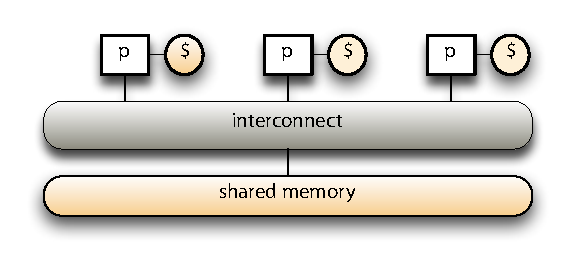
\includegraphics[width=.70\linewidth]{figures/shared-memory.pdf}
    \label{fig:shared-memory}
  \end{figure}
%
  \item for shared {\em address space} machine:
    \begin{itemize}
      \item replace caches with local/private memory
      \item cost: repeatedly accessed data should be copied to local storage
      \item not done much any more, but recently relevant thanks to hybrid CPU/GPGPU systems and
        the implementation details of nVidia chips
    \end{itemize}
%
  \end{itemize}
%
\end{frame}

% --------------------------------------
% programming a shared memory machine
\begin{frame}[fragile]
%
  \frametitle{Programming in a shared address space}
%
  \begin{itemize}
%
  \item the program creates and manages $p$ instruction streams (threads)
  \item each with a set of private variables
    \begin{itemize}
      \item registers, stack, cache
    \end{itemize}
%
  \item collectively with a set of shared variables
    \begin{itemize}
      \item statics, heap
    \end{itemize}
%
  \item communication is {\em implicit}: threads just access the shared memory locations
  \item synchronization is {\em explicit}: read/write flags, locks, semaphores
%
  \begin{figure}
    \centering
    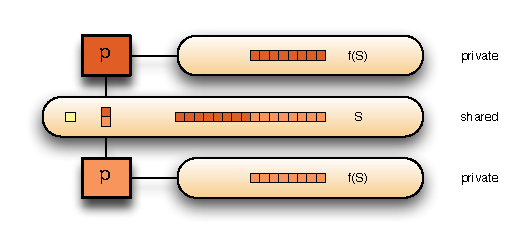
\includegraphics[width=\linewidth]{figures/reduction-shared.pdf}
    \label{fig:reduction-shared}
  \end{figure}
%
  \end{itemize}
%
\end{frame}

% --------------------------------------
% implementation of the reduction in a shared memory machine
\begin{frame}[fragile]
%
  \frametitle{Implementation in a shared address space}
%
  \begin{itemize}
%
  \item let's implement with two threads

    \vspace{.5em}
    \begin{minipage}{.40\linewidth}
      \begin{algorithm}[H]
%
        \footnotesize
        \dontprintsemicolon
        \nocaptionofalgo
        \setalcaphskip{0ex}
%
        \caption{\hspace{1em}thread 1}
        \vspace{.5em}
%
        $s \leftarrow 0$ \;
        $s_{1} \leftarrow 0$ \;
        \For{$i \leftarrow 1$ \KwTo $n/2-1$}{
          $s_{1} \leftarrow s_{1} + f(S[i])$ \;
        }
        $s \leftarrow s+s_{1}$ \;
%
        \vspace{.5em}
%
      \end{algorithm}
    \end{minipage}
%
    \hspace{.1\linewidth}
%
    \begin{minipage}{.40\linewidth}
      \begin{algorithm}[H]
%
        \footnotesize
        \dontprintsemicolon
        \nocaptionofalgo
        \setalcaphskip{0ex}
%
        \caption{\hspace{1em}thread 2}
        \vspace{.5em}
%
        $s \leftarrow 0$ \;
        $s_{2} \leftarrow 0$ \;
        \For{$i \leftarrow n/2$ \KwTo $n$}{
          $s_{2} \leftarrow s_{2} + f(S[i])$ \;
        }
        $s \leftarrow s+s_{2}$ \;
%
        \vspace{.5em}
      %
      \end{algorithm}
    \end{minipage}
    \vspace{.5em}
%
  \item what is wrong with this code? 
%
    \begin{itemize}
    \item {\em race condition}
    \item instructions from different threads can be executed in any order
    \item can you deduce all the possible values of $s$ after both threads finished executing?
    \item one possible solution is to place line 5 in a lock/load/modify/store/unlock block
    \end{itemize}
%
  \end{itemize}
%
\end{frame}

% --------------------------------------
% machine model 2: a distributed memory machine
\begin{frame}[fragile]
%
  \frametitle{Distributed memory machines}
%
  \begin{itemize}
%
  \item processors are all connected to their own private memory
  \item processors have no access to each other's memory, except through explicit exchanges
  \item each node is connected to a communication substrate: ethernet, myrinet, infiniband
%
  \begin{figure}
    \centering
    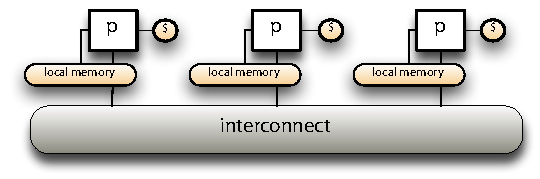
\includegraphics[width=.90\linewidth]{figures/distributed-memory.pdf}
    \label{fig:distributed-memory}
  \end{figure}
%
  \item all communication and synchronization is carried over the ``network''
%
  \end{itemize}
%
\end{frame}

% --------------------------------------
% programming a distributed memory machine
\begin{frame}[fragile]
%
  \frametitle{Programming in a distributed address space}
%
  \begin{itemize}
%
  \item message passing
    \begin{itemize}
      \item programs consists of a collection of $n$ {\em named} processes
        \begin{itemize}
        \item typically numbered 0 through $n-1$
        \item thread of control, local address space
        \item local variables, statics, heap
        \end{itemize}
      \item process communicate via {\em explicit} data exchanges
        \begin{itemize}
        \item matching pair of send/receive by source and destination processors respectively
        \item primitives for efficient implementation of many-to-exchanges
        \end{itemize}
      \item co\"ordination is implicit in every communication
      \item logically shared data must be {\em partitioned} among the local processes
    \end{itemize}
%
  \begin{figure}
    \centering
    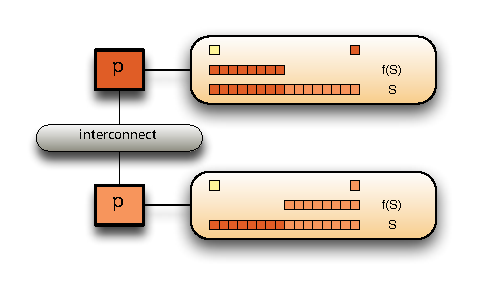
\includegraphics[width=.70\linewidth]{figures/reduction-distributed.pdf}
    \label{fig:reduction-distributed}
  \end{figure}
%
  \item standard libraries: MPI, the survivor
  \end{itemize}
%
\end{frame}

% --------------------------------------
% implementation of the reduction in a distributed memory machine
\begin{frame}[fragile]
%
  \frametitle{Implementation in a distributed address space}
%
  \begin{itemize}
%
  \item na\"ive implementation

    \vspace{.5em}
    \begin{minipage}{.40\linewidth}
      \begin{algorithm}[H]
%
        \footnotesize
        \dontprintsemicolon
        \nocaptionofalgo
        \setalcaphskip{0ex}
%
        \caption{\hspace{1em}processor 1}
        \vspace{.5em}
%
        $s_{1} \leftarrow 0$ \;
        \For{$i \leftarrow 1$ \KwTo $n/2-1$}{
          $s_{1} \leftarrow s_{1} + f(S[i])$ \;
        }
        \KwSend $s_{1}$ \KwTo $p_{2}$ \;
        $s_{2} \leftarrow \KwRecv\ \KwFrom\ p_{2}$ \;
        $s \leftarrow s_{1}+s_{2}$ \;
%
        \vspace{.5em}
%
      \end{algorithm}
    \end{minipage}
%
    \hspace{.1\linewidth}
%
    \begin{minipage}{.40\linewidth}
      \begin{algorithm}[H]
%
        \footnotesize
        \dontprintsemicolon
        \nocaptionofalgo
        \setalcaphskip{0ex}
%
        \caption{\hspace{1em}processor 2}
        \vspace{.5em}
%
        $s_{2} \leftarrow 0$ \;
        \For{$i \leftarrow n/2$ \KwTo $n$}{
          $s_{2} \leftarrow s_{2} + f(S[i])$ \;
        }
        \KwSend $s_{2}$ \KwTo $p_{1}$ \;
        $s_{1} \leftarrow \KwRecv\ \KwFrom\ p_{1}$ \;
        $s \leftarrow s_{2}+s_{1}$ \;
%
        \vspace{.5em}
      %
      \end{algorithm}
    \end{minipage}
    \vspace{.5em}
%
  \item what is wrong with this code? 
%
    \begin{itemize}
    \item {\em race condition}; more subtle than before
    \item pair up sends and receives to create logically atomic exchanges
    \item or use a many-to-many communication primitive, if available
    \end{itemize}
%
  \end{itemize}
%
\end{frame}

% end of file 

% -*- LaTeX -*-
% -*- coding: utf-8 -*-
%
% ~~~~~~~~~~~~~~~~~~~~~~~~~~~~~~~~~~~~~~~~~~~~~~~~~~~~~~~~~~~~~~~~~~~~~~~~~~~~~~
%
%                             michael a.g. aïvázis
%                      california institute of technology
%                      (c) 1998-2010  all rights reserved
%
% ~~~~~~~~~~~~~~~~~~~~~~~~~~~~~~~~~~~~~~~~~~~~~~~~~~~~~~~~~~~~~~~~~~~~~~~~~~~~~~
%

\lecture{Cost modeling and performance tradeoffs}{20100113}

% --------------------------------------
% generic parallel architecture
\begin{frame}[fragile]
%
  \frametitle{Time, parallelism and computational work}
%
  \begin{itemize}
  \item recall our embarrassingly parallel reduction: 
    \begin{itemize}
    \item given a function $f$ and a sequence of numbers $S$ of length $N$, evaluate
    \[
    s = \sum_{i=0}^{N-1}f(S_{i})
    \]
    \end{itemize}
%
  \item initial parallelism profile for a simple mapping, assuming that
    \begin{itemize}
    \item the computation of $f(S)$ is the parallel task
    \item the summation is sequential
    \end{itemize}
%
    \begin{minipage}{.45\linewidth}
      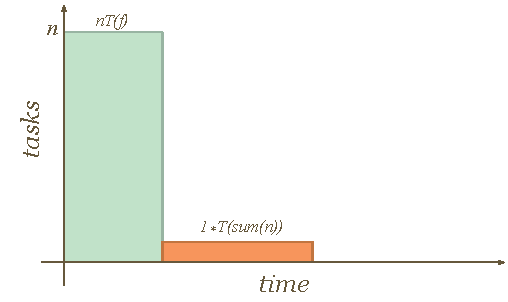
\includegraphics[scale=0.6]{figures/reduction-parallel-work.pdf}
    \end{minipage}
    $\longrightarrow$
    \begin{minipage}{.45\linewidth}
      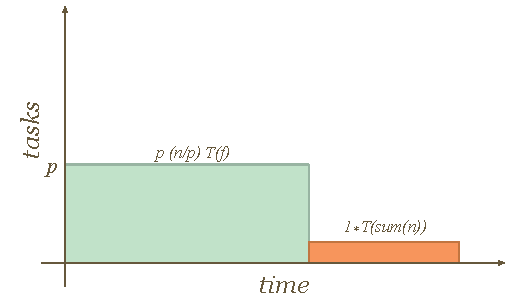
\includegraphics[scale=0.6]{figures/reduction-partitioned-work.pdf}
    \end{minipage}
%
  \item shaded area is $w$, the {\em computational work}
%
  \end{itemize}
%
\end{frame}

% --------------------------------------
% speedup and efficiency
\begin{frame}[fragile]
%
  \frametitle{Metrics: speedup and efficiency}
%
  \begin{itemize}
%
    \item let
      \begin{itemize}
        \item $T_{1}$ be the sequential execution time on one processor
        \item $T_{p}$ be the parallel execution time on $p$ processors
      \end{itemize}
%
    \item define
      \begin{itemize}
        \item {\em speedup}: \[\sigma \defeq T_{1}/T_{p}\]
        \item {\em efficiency}: \[\eta \defeq T_{1}/(p T_{p})\]
        \item related through $\eta = \sigma/p$ and $\sigma = \eta p$
      \end{itemize}
%
    \item pseudo-theorems: $\sigma \leq p$ and $\eta \leq 1$
      \begin{itemize}
        \item but {\em speedup anomalies} can occur if resources increase with $p$ causing an
          increase in the effective computation rate
        \item example: for large enough $p$, your problem may fit entirely in the L2 cache
        \item {\em sweet spots} like that abound; the craftsman knows how to
          \begin{itemize}
            \item implement the solution in a portable manner
            \item expose enough controls to be able to tune the implementation to a given
              architecture
          \end{itemize}
      \end{itemize}
%
  \end{itemize}
%
\end{frame}

% --------------------------------------
% amdahl's law
%
\begin{frame}[fragile]
%
  \frametitle{The bad news: Amdahl's law}
%
  \begin{minipage}{.55\linewidth}
    \begin{itemize}
%
    \item consider a solution that consists of two parts
      \begin{itemize}
      \item a serial fraction $s$ with $0 \leq s \leq 1$
      \item a $p$-fold parallel fraction $1-s$
      \end{itemize}
%
    \item for a fixed problem size, Amdahl's law relates $T_{p}$, $\sigma$ and $\eta$ to
      $T_{1}$ and $s$
      \begin{eqnarray*}
        T_{p}  & = & s T_{1} + (1-s) T_{1} / p \\
        \sigma & = & \frac{p}{sp + (1-s)} \\
        \eta & = & \frac{1}{sp + (1-s)}
      \end{eqnarray*}
%
    \item with corollaries $\sigma_{\infty} = \frac{1}{s}$ and $\eta_{\infty} = 0$
    \end{itemize}
  \end{minipage}
 %
  \hfill
  \begin{minipage}{.40\linewidth}
    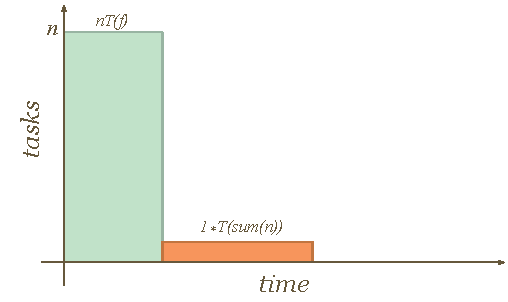
\includegraphics[width=1.2\linewidth]{figures/reduction-parallel-work.pdf}
    \vspace{2em}

    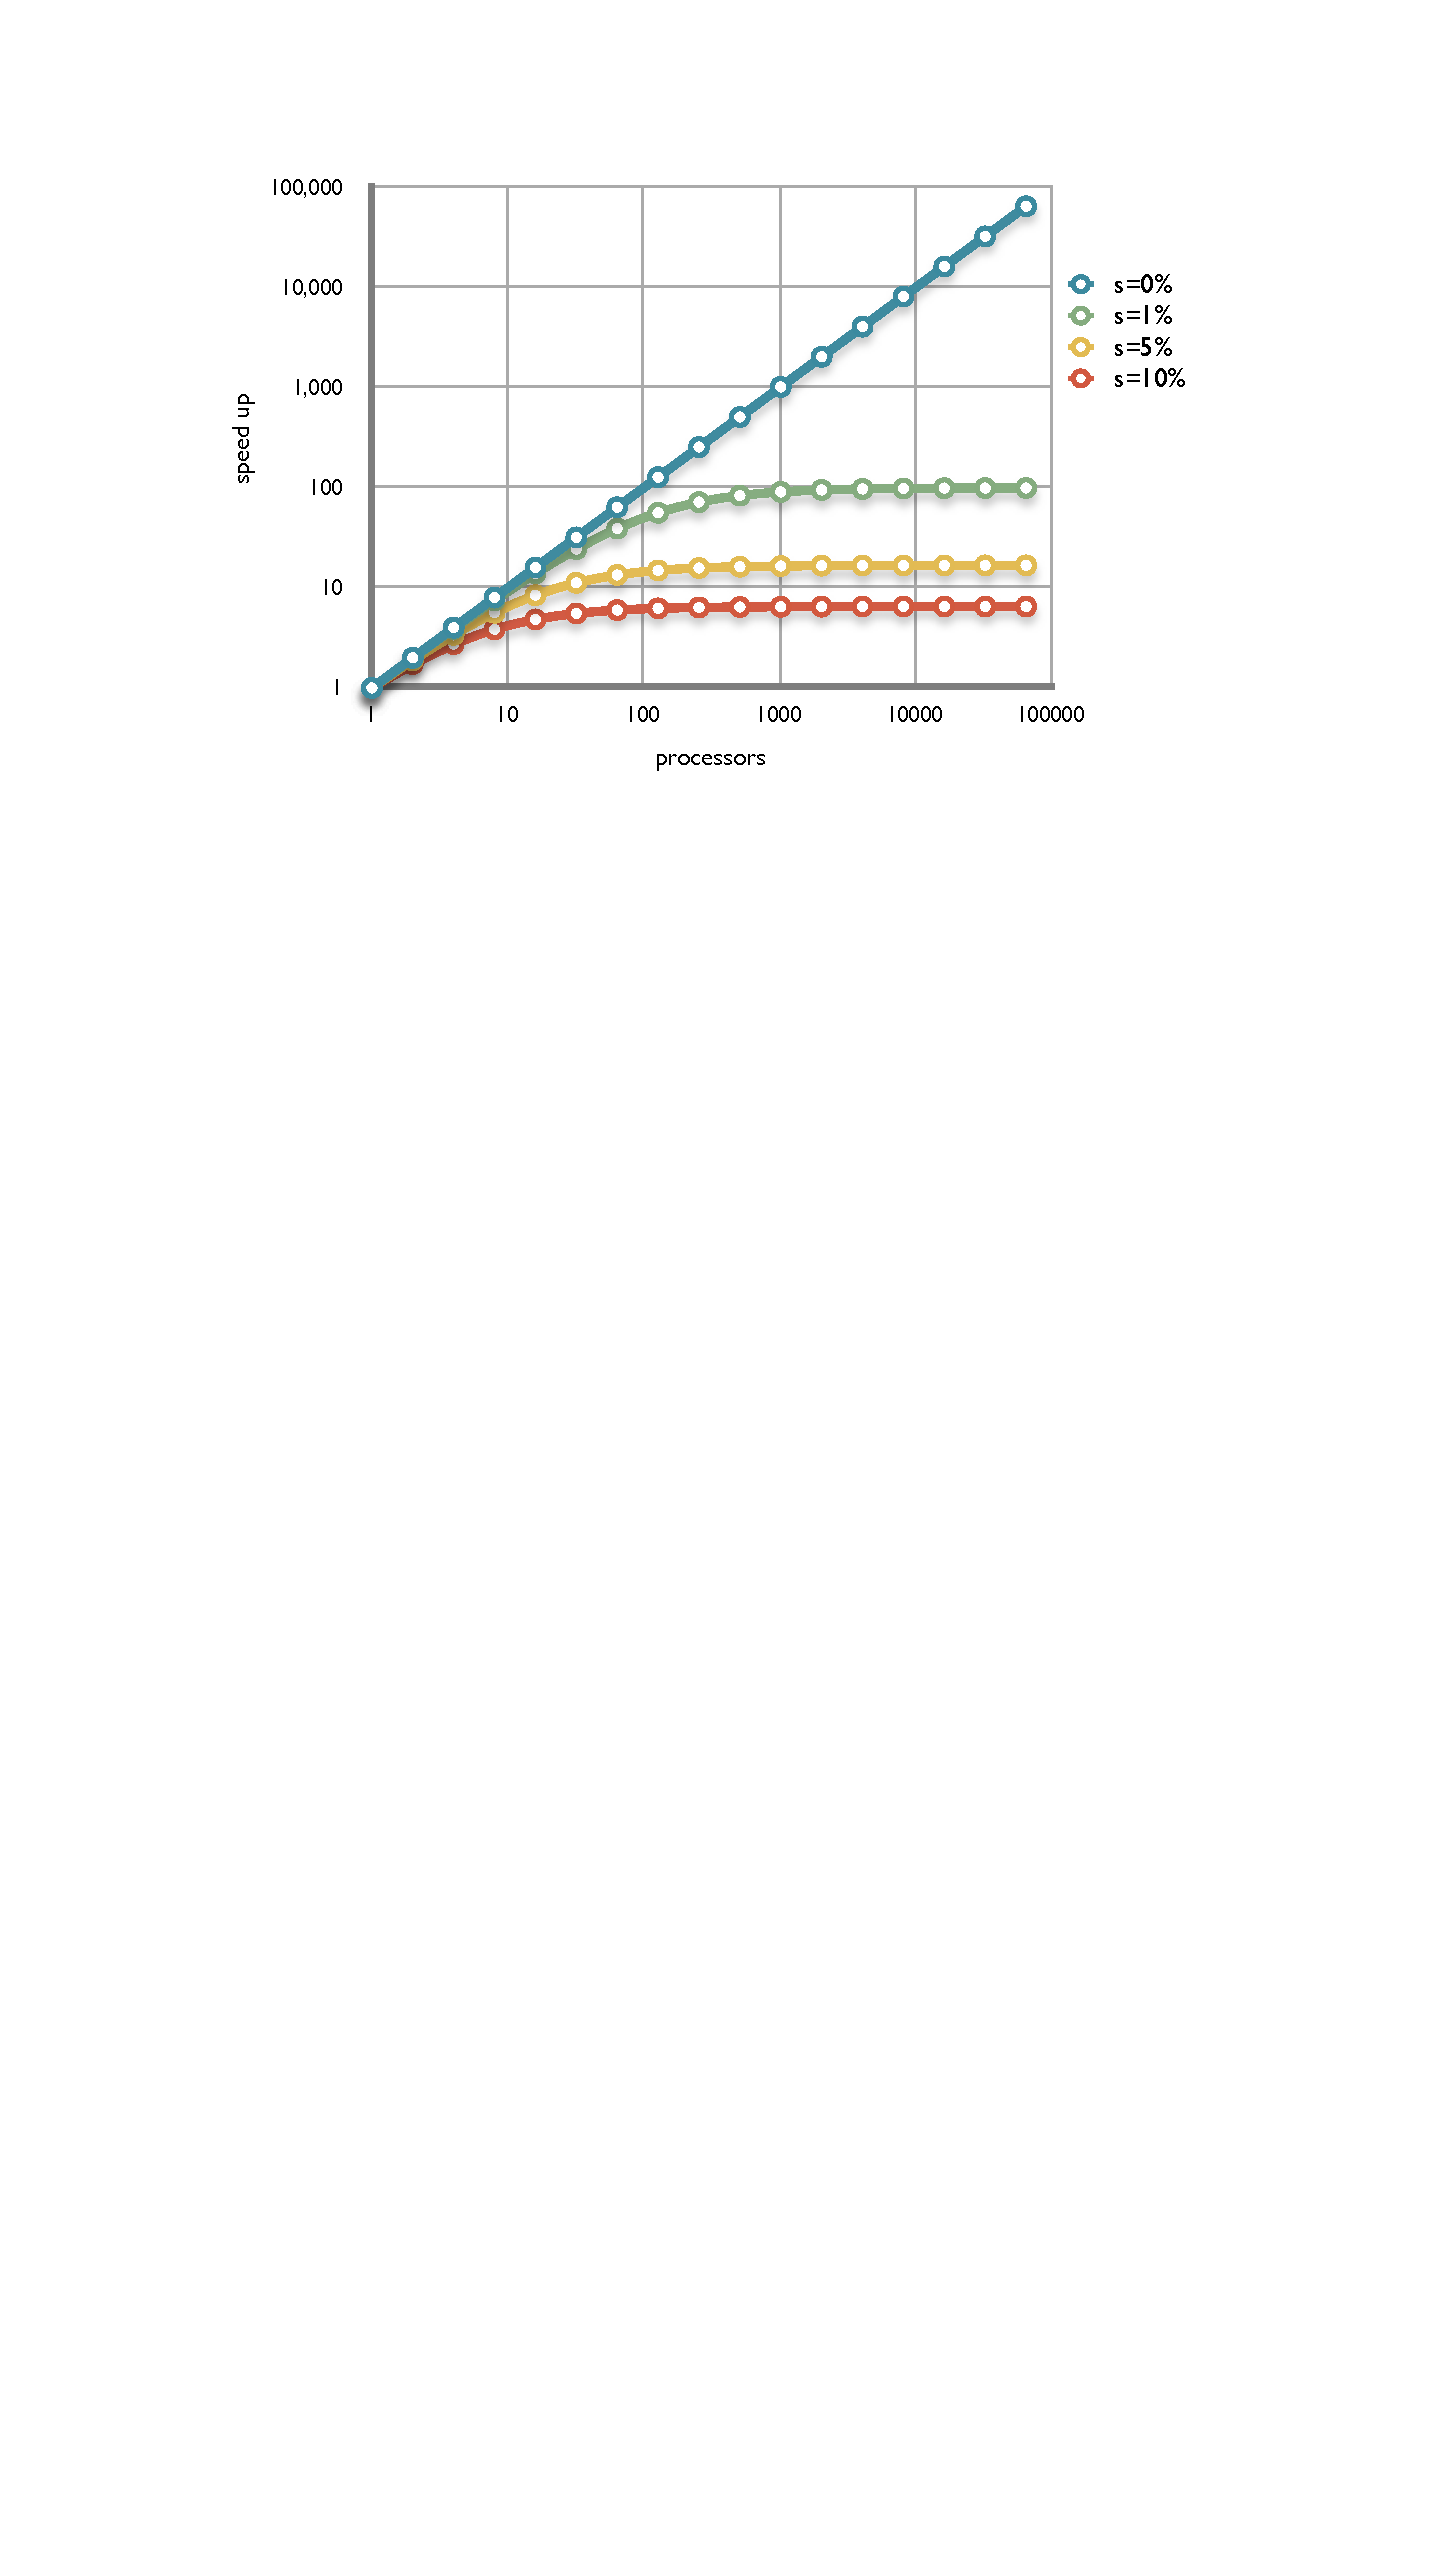
\includegraphics[width=1.2\linewidth]{figures/amdahl.pdf}
  \end{minipage}
%
\end{frame}

% --------------------------------------
% scaling and isoefficiency
\begin{frame}[fragile]
%
  \frametitle{Beating Amdahl's law}
%
  \begin{itemize}
  \item Amdahl's law holds if either
    \begin{itemize}
      \item the problem size is fixed
      \item the serial fraction $s$ is not a function of $p$
    \end{itemize}
%
  \item {\em weak scaling}: let the problem size grow with $p$
    \begin{itemize}
    \item larger computers are used to solve larger problems
    \item the effective serial fraction {\em decreases} with problem size
    \item the right scaling metric would be constant, or properly bounded, as $p \rightarrow
      \infty$
    \end{itemize}
%
  \item {\em isoefficiency}
    \begin{itemize}
      \item how rapidly must problem size grow so that $\eta$ is constant as $p$ increases?
      \item since $\eta = T_{1}/(pT_{p})$, constant efficiency implies
        \[
        T_{1} = c (p T_{p})
        \]
        for some constant $c$
      \item $T_{1}$ measures the sequential work, so the above relation determines your
        implementation's {\em isoefficiency function}
    \end{itemize}
%
  \end{itemize}
%
\end{frame}



% --------------------------------------
% algorithmic trade-offs
\begin{frame}[fragile]
%
  \frametitle{Algorithmic improvements}
%
  \begin{itemize}
%
  \item getting smarter is the best way to improve $\sigma$ and $\eta$
    \begin{itemize}
      \item reduce the sequential fraction $s$
      \item what are the effects on communication and locality?
    \end{itemize}
%
  \item parallelize the partial sums
    \begin{figure}
      \centering
      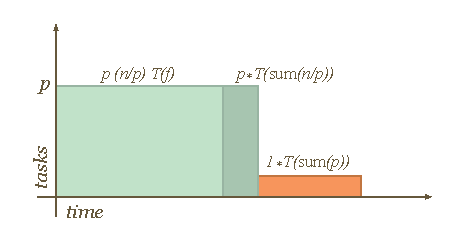
\includegraphics[scale=0.70]{figures/reduction-partial-sum.pdf}
    \end{figure}
%
  \item parallelize the final sum using a {\em reduction tree}
    \begin{figure}
      \centering
      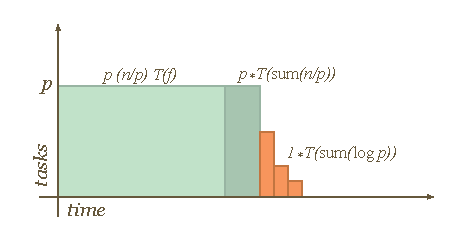
\includegraphics[scale=0.70]{figures/reduction-tree-sum.pdf}
    \end{figure}
%
  \end{itemize}
%
\end{frame}

% --------------------------------------
% load balance
\begin{frame}[fragile]
%
  \frametitle{Load balance}
%
  \begin{itemize}
%
  \item non-optimal task distributions show up as {\em load imbalance}
    \begin{figure}
      \centering
      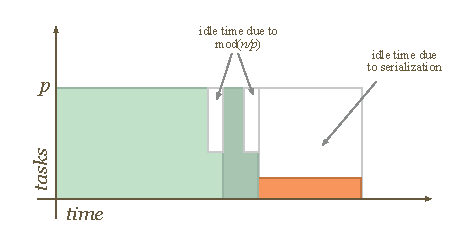
\includegraphics[scale=1.0]{figures/reduction-load-imbalance.pdf}
    \end{figure}
%
  \item excessive coarsening tends to increase load imbalance
  \item so can inappropriate mapping
  \item synchronization also causes load imbalance (see later slide)
  \item new upper bound for the speedup
    \[
    \sigma \leq \frac{w_{1}}{{\rm max\ }_{p}(w_{p} + {\rm idle})}
    \]
      
  \end{itemize}
%
\end{frame}

% --------------------------------------
% overhead
\begin{frame}[fragile]
%
  \frametitle{Parallelization overhead}
%
  \begin{itemize}
%
  \item there is always some extra work that is not present in the sequential implementation
    \begin{figure}
      \centering
      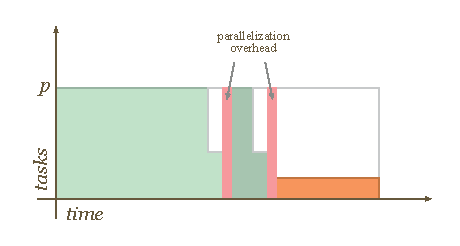
\includegraphics[scale=1.0]{figures/reduction-overhead.pdf}
    \end{figure}
%
  \item orchestration, management, bookkeeping
    \[
    \sigma \leq \frac{w_{1}}{{\rm max\ }_{p}(w_{p} + {\rm idle} + {\rm overhead})}
    \]
      
%
  \end{itemize}
%
\end{frame}

% --------------------------------------
% communication and synchronization costs
\begin{frame}[fragile]
%
  \frametitle{Communication and synchronization costs}
%
  \begin{itemize}
%
  \item communication is required for data movement and synchronization
    \begin{figure}
      \centering
      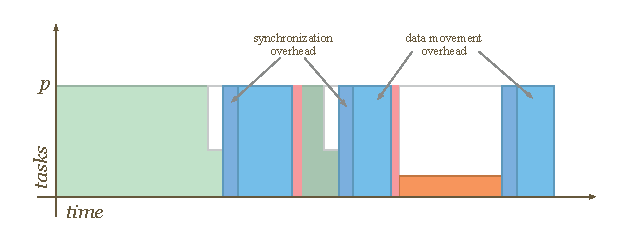
\includegraphics[scale=0.75]{figures/reduction-comsync.pdf}
    \end{figure}
%
  \item the cost is modeled by
    \[
    T_{c} = \lambda + \beta L
    \]
    where the {\em latency} $\lambda$ measures the communication startup cost, $\beta$ is the
    bandwidth of the interconnect and $L$ is the message length in {\em words} 
%
  \item the speedup is now bounded by
    \[
    \sigma \leq \frac{w_{1}}{{\rm max\ }_{p}(w_{p} + {\rm idle} + {\rm overhead} + {\rm comm})}
    \]
%      
  \end{itemize}
%
\end{frame}

% --------------------------------------
% reducing communication costs
\begin{frame}[fragile]
%
  \frametitle{Reducing communication costs}
%
  \begin{itemize}
%
  \item multiple strategies
%
  \item co\"ordinating placement of work and the associated data to minimize inter-process
    dependencies
    \begin{figure}
      \centering
      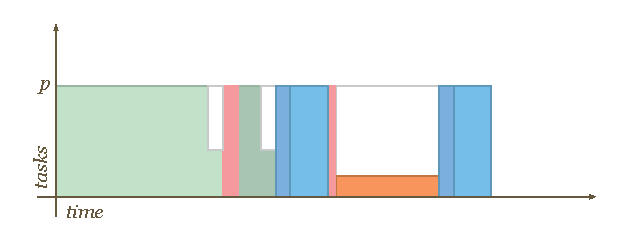
\includegraphics[scale=0.5]{figures/reduction-comsync-replication.pdf}
    \end{figure}
%
  \item trading memory for efficiency by replicating data
%
  \item trading cpu for efficiency by doing redundant work
    \begin{figure}
      \centering
      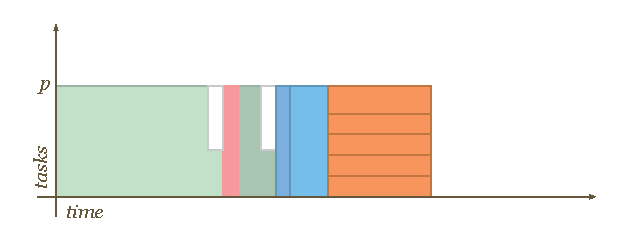
\includegraphics[scale=0.5]{figures/reduction-comsync-redundancy.pdf}
    \end{figure}
%
  \item improving communication efficiency by tuning the cost factors
    \begin{itemize}
    \item communication frequency, message size, contention, architecture specific
      optimizations
    \end{itemize}
%
  \end{itemize}
%
\end{frame}

% --------------------------------------
% tension
\begin{frame}[fragile]
%
  \frametitle{Optimizing speedup and efficiency}
  \begin{itemize}
%
    \item the goal is to minimize the denominator
      \[
      \sigma \leq \frac{w_{1}}{{\rm max\ }_{p}(w_{p} + {\rm idle} + {\rm overhead} + {\rm comm})}
      \]
      \begin{itemize}
        \item but its parts are in tension: minimizing one happens at the expense of another
      \end{itemize}
%
  \item fine grain decomposition and intelligent mapping tend to minimize load imbalance at the
    cost of increased communication
    \begin{itemize}
    \item coarser grains imply larger message size and fewer synchronization events
    \item for many problems communication costs decrease as surface to volume
    \end{itemize}
%
  \item na\"ive static partitioning reduces redundant work but cause load imbalance
%
  \end{itemize}
%
\end{frame}

% --------------------------------------
% the good news
\begin{frame}[fragile]
%
  \frametitle{The good news}
%
  \begin{itemize}
%
  \item the basic work unit of a parallel algorithm may be more efficient (and better
    performing) than the sequential equivalent
    \begin{itemize}
    \item only a small fraction of typical problems fits in L2 cache
    \item single node performance {\em requires} partitioning
    \item just like the parallel implementation
    \item don't be surprised by the poor quality of your sequential version after you see
      your parallel implementation
    \end{itemize}
%
  \item communication can be interleaved with computation
    \begin{itemize}
    \item better algorithms on today's complicated memory hierarchies
    \end{itemize}
%
    \item parallel algorithms may lead to better sequential ones
      \begin{itemize}
        \item e.g.~parallel search may explore configuration space more effectively
      \end{itemize}
%
  \end{itemize}
%
\end{frame}

% end of file 

% -*- LaTeX -*-
% -*- coding: utf-8 -*-
%
% ~~~~~~~~~~~~~~~~~~~~~~~~~~~~~~~~~~~~~~~~~~~~~~~~~~~~~~~~~~~~~~~~~~~~~~~~~~~~~~
%
%                             michael a.g. aïvázis
%                      california institute of technology
%                      (c) 1998-2010  all rights reserved
%
% ~~~~~~~~~~~~~~~~~~~~~~~~~~~~~~~~~~~~~~~~~~~~~~~~~~~~~~~~~~~~~~~~~~~~~~~~~~~~~~
%

\lecture{Software engineering survival skills}{20100115}

% --------------------------------------
% 
\begin{frame}[fragile]
%
  \frametitle{Software engineering survival skills}
%
  \begin{itemize}
%
  \item class hardware
    \begin{itemize}
    \item your laptop
    \item mind-meld
    \item shc
    \end{itemize}
%
  \item access
    \begin{itemize}
    \item login
    \item shell
    \item setting up access to what you need
    \end{itemize}
%
  \item source control
    \begin{itemize}
    \item why bother?
    \item styles and workflows
    \item available tools
    \end{itemize}
%
  \item writing your own
    \begin{itemize}
    \item editing: emacs, vi, ?
    \item compiling and linking
    \item running
    \end{itemize}
%
  \item configuration management
    \begin{itemize}
    \item automating the build process
    \item config
    \end{itemize}
%
  \end{itemize}
%
\end{frame}

% --------------------------------------
% shell
\begin{frame}[fragile]
%
  \frametitle{Working with the shell}
%
  \begin{itemize}
%
  \item here is an example shell session
    \begin{bash}
#
# ls
Make.mm                 content                 outline.html            syllabus.html
acm114.html             images                  references.html
assignments.html        index.html              scripts
calendar.html           instructor.html         styles
    \end{bash}
%
  \end{itemize}
%
\end{frame}

% end of file 

% -*- LaTeX -*-
% -*- coding: utf-8 -*-
%
% ~~~~~~~~~~~~~~~~~~~~~~~~~~~~~~~~~~~~~~~~~~~~~~~~~~~~~~~~~~~~~~~~~~~~~~~~~~~~~~
%
%                             michael a.g. aïvázis
%                      california institute of technology
%                      (c) 1998-2010  all rights reserved
%
% ~~~~~~~~~~~~~~~~~~~~~~~~~~~~~~~~~~~~~~~~~~~~~~~~~~~~~~~~~~~~~~~~~~~~~~~~~~~~~~
%

\pagestyle{headandfoot}
\runningfootrule
\firstpageheader{ACM/CS 114}{Assignment 1}{Due: 20 Jan 2010}
\runningheader{}{}{}
\firstpagefooter{}{}{}
\runningfooter{ACM/CS 114}{Assignment 1}{\thepage}

\begin{questions}

% --------------------------------------
% merge sort
\question
\mergesort\ is an example of a {\em divide-and conquer} algorithm. The algorithm
sorts an input sequence $S$ of numbers along the following steps:
%
\begin{itemize}
\item {\em divide}: split $S$ into two parts of roughly equal length,
\item {\em conquer}: sort the subsequences recursively,
\item {\em combine}: merge the two sorted subsequences to produce the sorted output.
\end{itemize}
%
In pseudocode:
%
\begin{center}
  \begin{minipage}{.5\linewidth}
    \begin{algorithm}[H]
      \label{alg:merge-sort}
%
      \dontprintsemicolon
      %\nocaptionofalgo
      \setalcaphskip{0ex}
%
      \caption{\mergesort($S$, $p$, $r$)}
      \vspace{.5em}
%
      \If{$p < r$}{
        $q \leftarrow \lfloor (p+r)/2 \rfloor$ \;
        \mergesort($S$, $p$, $q$) \;
        \mergesort($S$, $q+1$, $r$) \;
        \merge($S$, $p$, $q$, $r$) \;
      }
%
      \vspace{.5em}
%
    \end{algorithm}
  \end{minipage}
\end{center}
%
\begin{parts}

\part Explain the role of $p$ and $r$ in the algorithm specification. What values should they
have upon initial invocation of the algorithm?

\part Write \merge. It was claimed in class that \merge\ can be implemented to run in
$\Theta(r-p+1)$ time. How does your implementation compare?

\part Implement \mergesort\ in a language of your choice. 
\begin{subparts}
  \subpart Write a driver that invokes it with $S = (5, 2, 4, 6, 1, 3)$.
  \subpart Build a container with $10^6$ random numbers. Sort it using your implementation.
\end{subparts}

\end{parts}

% --------------------------------------
% reduction 
\def\Li{\mbox{\rm Li}_{2}}
\def\len{\mbox{\rm length}}
\def\dilog{\mbox{\tt dilog}}
\def\sdlog{\mbox{\tt sdilog}}

\question Consider the function $\Li$ defined for $|z| \leq 1$ by
\[
\Li(z) \bydef
     \sum_{n=1}^{\infty} \frac{z^{n}}{n^{2}}
     =
     z + \frac{z^{2}}{2^{2}} + \frac{z^{3}}{3^{2}} + \frac{z^{4}}{4^{2}} + \cdots
\]

\begin{parts}

\part In the language of your choice, implement a procedure \dilog($z$, $n$) that computes the
sum of the first $n$ terms of the series for the given floating point number $z$.

\part Implement a procedure \sdlog($Z$, $n$) that accepts a sequence $Z$ of floating point
numbers and computes the sum
\[
\sdlog(Z, n) \bydef \sum_{z \in Z} \dilog(z, n)
\]

\part Build a cost model for \sdlog\ as a function of $n$ and $m \bydef \len(Z)$. Assume that
additions and subtractions cost $c_{+}$ each, multiplications and divisions cost $c_{\times}$
each, and that raising a number to the $n$th power costs $c_{\star}$.

\end{parts}
        
\end{questions}

% end of file 

% -*- LaTeX -*-
% -*- coding: utf-8 -*-
%
% ~~~~~~~~~~~~~~~~~~~~~~~~~~~~~~~~~~~~~~~~~~~~~~~~~~~~~~~~~~~~~~~~~~~~~~~~~~~~~~
%
%                             michael a.g. aïvázis
%                      california institute of technology
%                      (c) 1998-2010  all rights reserved
%
% ~~~~~~~~~~~~~~~~~~~~~~~~~~~~~~~~~~~~~~~~~~~~~~~~~~~~~~~~~~~~~~~~~~~~~~~~~~~~~~
%

\lecture{Programming with pthreads - part 2}{20100122}

% --------------------------------------
% hello world
\begin{frame}[fragile]
%
  \frametitle{Hello world}
  \label{slide:hello-world-threads}
%
  \begin{C}
#include <pthread.h>
#include <stdio.h>
#define THREADS 10

void* hello(void* threadID) {
    long id = (long) threadID;
    printf("hello from %02ld/%0d\n", id, THREADS);
    pthread_exit(NULL);
    return NULL;
}

int main(int argc, char* argv[]) {
    long id;
    int status;
    pthread_t threads[THREADS];

    for (id=0; id<THREADS; id++) {
        printf("creating thread %02ld\n", id);
        status = pthread_create(&threads[id], NULL, hello, (void*) id);
        if (status) {
            printf("error %d in pthread_create\n", status);
        }
    }
    /* there is a problem here... */
    pthread_exit(NULL);
    return 0;
}
  \end{C}
%
\end{frame}

% --------------------------------------
% joining and detaching threads
\begin{frame}[fragile]
%
  \frametitle{Joining and detaching}
%
  \begin{itemize}
%
  \item in the example in \slideref{hello-world-threads}, the main thread exits without knowing whether
    any of the threads it spawned have finished
    \begin{itemize}
    \item saying ``hello'' is asynchronous
    \item but gathering the results of parallel calculations normally isn't
    \end{itemize}
%
  \item {\em thread synchronization} can be achieved using \function{pthread\_join}
    \begin{itemize}
      \item the \function{pthread\_create} caller saves the thread id
      \item the thread is scheduled, executes, and calls \function{pthread\_exit}
      \item any other thread can wait for this thread to finish by calling
        \function{pthread\_join} with the saved thread id and also retrieve the termination
        status
    \end{itemize}
%
  \item for this to work, a thread must be {\em joinable}
    \begin{itemize}
    \item controlled by the thread creation attributes
    \item for portability, you should always mark your joinable threads explicitly
    \end{itemize}
%
%
    \item a thread that will never be joined may be {\em detached}
      \begin{itemize}
      \item by setting the corresponding attribute during thread creation
      \item or, by calling \function{pthread\_detach} at any point
      \item detaching a thread saves some system resources
      \end{itemize}
        
  \end{itemize}
%
\end{frame}

% --------------------------------------
% mutexes
\begin{frame}[fragile]
%
  \frametitle{Creating mutexes}
%
  \begin{itemize}
%
  \item a {\em mutex} is a locking mechanism that helps guarantee exclusive access to a section
    of code, most often to control access to shared variables
%
  \item mutexes are created using
%
    \begin{C}
int pthread_mutex_init(
    pthread_mutex_t* mutex, const pthread_mutexattr_t* attr);
    \end{C}
%
    \begin{itemize}
    \item they start out unlocked
    \item the \identifier{attr} enables more advanced (but perhaps non-portable) use
    \end{itemize}
%
  \item mutexes are destroyed using
%
    \begin{C}
int pthread_mutex_destroy(pthread_mutex_t* mutex);
    \end{C}
%
    \begin{itemize}
    \item destroy mutexes you are no longer using to prevent resource leakage
    \end{itemize}
%
  \end{itemize}
%
\end{frame}

% --------------------------------------
% mutex manipulation
\begin{frame}[fragile]
%
  \frametitle{Locking and unlocking mutexes}
%
  \begin{itemize}
%
  \item threads manipulate mutexes through
%
    \begin{C}
int pthread_mutex_lock(pthread_mutex_t* mutex);
int pthread_mutex_trylock(pthread_mutex_t* mutex);
int pthread_mutex_unlock(pthread_mutex_t* mutex);
    \end{C}
%
  \item \identifier{pthread\_mutex\_lock} attempts to gain exclusive access
    \begin{itemize}
    \item if the mutex is unlocked, it locks it and returns
    \item otherwise, it blocks until the mutex is unlocked; when the mutex is unlocked, it
      locks it and returns
    \end{itemize}
%
  \item \identifier{pthread\_mutex\_unlock} attempts to release a mutex
    \begin{itemize}
    \item if it was previously locked by this thread, the mutex is unlocked
    \item if it was not previously locked, the call returns with an error code
    \item if it was locked, but not by the calling thread, the call returns an error code
    \end{itemize}
%
  \item \identifier{pthread\_mutex\_trylock} attempts to lock the mutex
    \begin{itemize}
    \item if it is unlocked, the call locks it and returns
    \item if it is locked, the call returns immediately with a {\em busy} error code
    \end{itemize}
%
  \item locking and unlocking mutexes is explicitly orchestrated by the programmer
  \item when multiple threads are blocked waiting for a mutex, there is no way to predict which
    one will succeed when the mutex becomes available
%
  \end{itemize}
%
\end{frame}

% --------------------------------------
% sum of squares
\begin{frame}[fragile]
%
  \frametitle{Example reduction using threads}
  \label{slide:squares-threads}
%
  \begin{C}[basicstyle=\tt\bfseries\tiny]
#include <pthread.h>
#include <stdio.h>
#define THREADS 10
/* global variables -- yuck! */
long sum = 0;
pthread_mutex_t mutex;
/* worker */
void* squares(void* threadID) {
    long id = (long) threadID;
    pthread_mutex_lock(&mutex);
    sum += id*id;
    pthread_mutex_unlock(&mutex);
    pthread_exit(NULL);
    return NULL;
}
/* main program */
int main(int argc, char* argv[]) {
    long id;
    pthread_t threads[THREADS];
    pthread_mutex_init(&mutex, NULL);
    /* create some threads */
    for (id=0; id<THREADS; id++) {
        pthread_create(&threads[id], NULL, squares, (void*) id);
    }
    /* wait for them  to finish */
    for (id=0; id<THREADS; id++) {
        pthread_join(threads[id], NULL);
    }
    /* print the result */
    printf("sum = %ld\n", sum);
    /* exit */
    pthread_exit(NULL);
    return 0;
}
  \end{C}
%
\end{frame}

% --------------------------------------
% condition variables
\begin{frame}[fragile]
%
  \frametitle{Condition variables}
%
  \begin{itemize}
%
  \item condition variables build upon mutexes to enable threads to signal each other when some
    condition is met
%
  \item they are created using
%
    \begin{C}
int pthread_cond_init(
    pthread_cond_t* condition, const pthread_condattr_t* attr);
    \end{C}
%
  \item and destroyed using
%
    \begin{C}
int pthread_cond_destroy(pthread_cond_t* condition);
    \end{C}
%
  \end{itemize}
%
\end{frame}

% --------------------------------------
% using condition variables
\begin{frame}[fragile]
%
  \frametitle{Using condition variables}
%
  \begin{itemize}
%
  \item the following three routies implement the condition variable semantics
%
    \begin{C}
int pthread_cond_wait(pthread_cond_t* cond, pthread_mutex_t* mutex);
int pthread_cond_signal(pthread_cond_t* cond);
int pthread_cond_broadcast(pthread_cond_t* cond);
    \end{C}
%
  \item \identifier{pthread\_cond\_wait} blocks the calling thread until the specified
    condition is {\em signaled}
    \begin{itemize}
    \item it must be called with the mutex locked by the calling thread
    \item \identifier{pthread\_cond\_wait} releases the lock while the thread is blocked
    \item after the matching signal is received, the thread is awakened and the mutex locked
    \item the thread is responsible for releasing the mutex when it is done
    \end{itemize}
%
  \item \identifier{pthread\_cond\_signal} wakes up a thread that is waiting for the given
    condition variable
    \begin{itemize}
    \item mutex must be locked before calling it
    \item mutex must be unlocked after signaling, so blocking threads can be awakened
    \end{itemize}
%
  \item \identifier{pthread\_cond\_broadcast} can be used instead if multiple threads are
    waiting for a signal
%
  \end{itemize}
%
\end{frame}

% --------------------------------------
% condition variable caveats
\begin{frame}[fragile]
%
  \frametitle{Condition variable caveats}
%
  \begin{itemize}
%
  \item be careful with condition variables; make sure that
    \begin{itemize}
    \item a thread has called \identifier{pthread\_cond\_wait} before any thread
      calls \identifier{pthread\_cond\_signal}
    \item the mutex associated with the condition is locked before calling
      \identifier{pthread\_cond\_wait}, otherwise it might {\em not block}
    \item the thread that calls \identifier{pthread\_cond\_signal} unlocks the associated
      mutex, otherwise the threads waiting for the signal will continue to block
    \end{itemize}
%
%
  \end{itemize}
%
\end{frame}

% --------------------------------------
% the attribute interface
\begin{frame}[fragile]
%
  \frametitle{Attributes of threads, mutexes and condition variables}
%
  \begin{itemize}
%
  \item threads, mutexes and condition variables have associated attribute structures that can
    be used to tune the default creation parameters
%
  \item they are created and destroyed using
%
    \begin{C}
int pthread_attr_init(pthread_attr_t* attr);
int pthread_attr_destroy(pthread_attr_t* attr);

int pthread_mutexattr_init(pthread_mutexattr_t* attr);
int pthread_mutexattr_destroy(pthread_mutexattr_t* attr);

int pthread_condattr_init(pthread_condattr_t* attr);
int pthread_condattr_destroy(pthread_condattr_t* attr);
    \end{C}
%
  \item typically, the defaults are adequate and tuned to the details of the operating system
%
  \item if you make excessive use of the stack, e.g.~large arrays as local variable or deep
    recursion, you might want to know about
%
    \begin{C}
int pthread_attr_getstacksize(pthread_attr_t* attr, size_t* size);
int pthread_attr_setstacksize(pthread_attr_t* attr, size_t size);
    \end{C}
%
  \end{itemize}
%
\end{frame}

% --------------------------------------
% miscellaneous
\begin{frame}[fragile]
%
  \frametitle{Other useful routines}
%
  \begin{itemize}
%
  \item a thread can access its unique id assigned by the system by calling 
%
    \begin{C}
pthread_t pthread_self(void);
    \end{C}
%
  \item since system thread ids are opaque types, you cannot use \operator{==} to compare
    them; instead, use
%
    \begin{C}
int pthread_equal(pthread_t id1, pthread_t id2);
    \end{C}
%
  \item you can place all thread initialization code in a startup routine and call
%
    \begin{C}
int pthread_once(pthread_once_t* control_structure, void (*startup_routine)(void));
    \end{C}
%
  \end{itemize}
%
\end{frame}

% --------------------------------------
% template
\begin{frame}[fragile]
%
  \frametitle{Advanced topics}
%
  \begin{itemize}
%
  \item there is quite a bit more in the standard
%
  \item {\em keys}: creating and accessing per-thread data
    \begin{itemize}
    \item as the code get more complicated, it becomes increasingly difficult to pass complete
      thread-specific information from function to function
    \item possible solutions:
      \begin{itemize}
      \item the \fortran\ syndrome, where subroutines end up having dozens of arguments
      \item global variables
      \item an associative container that allows each thread to store and retrieve arbitrary
        data
      \end{itemize}
%
    \end{itemize}
%
    \item finer control over thread scheduling
      \begin{itemize}
      \item scheduling algorithms and priorities are implementation dependent
      \item there are routines in the standard that enable explicit tuning
      \item the standard guarantees that the routines will be {\em available}, but they don't
        have to be {\em implemented}
      \end{itemize}
%
    \item condition variable sharing across processes
%
    \item explicitly canceling threads
%
    \item the somewhat complicated interactions between threads and signals
%
    \item other synchronization constructs: barriers and read/write locks
%
  \end{itemize}
%
\end{frame}

% --------------------------------------
% summary
\begin{frame}[fragile]
%
  \frametitle{Summary}
%
  \begin{itemize}
%
  \item well-designed threaded programs must follow the same strategy as any other concurrent
    program
    \begin{figure}
      \centering
      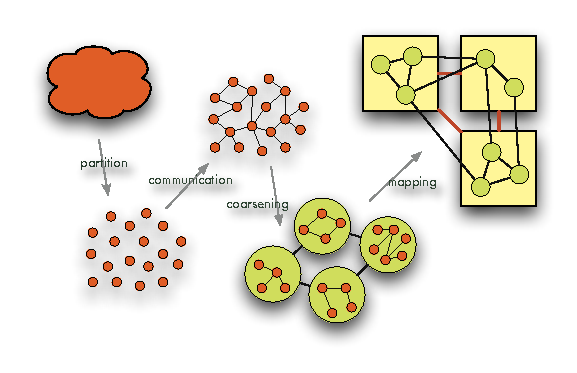
\includegraphics[scale=0.5]{figures/parallelization-steps.pdf}
      \label{fig:parallelization-steps-threads}
    \end{figure}
    \vspace{-1.75em}
%
    \begin{itemize}
    \item identify the work that can be done concurrently
    \item partition it in terms of work units, the fine grain tasks
    \item analyze the communication patterns among work units with an eye for critical sections
      and protecting shared data structures
    \item coarsen into threads, define the mutex categories and synchronization points
    \item let the OS schedule the threads onto physical processors
    \end{itemize}
%
  \item debugging threaded programs is very difficult
    \begin{itemize}
    \item preventing bugs through careful design is critical
    \item so is instrumenting the program to gain confidence in its execution
    \end{itemize}
%
  \end{itemize}
%
\end{frame}

% end of file 

% -*- LaTeX -*-
% -*- coding: utf-8 -*-
%
% ~~~~~~~~~~~~~~~~~~~~~~~~~~~~~~~~~~~~~~~~~~~~~~~~~~~~~~~~~~~~~~~~~~~~~~~~~~~~~~
%
%                             michael a.g. aïvázis
%                      california institute of technology
%                      (c) 1998-2010  all rights reserved
%
% ~~~~~~~~~~~~~~~~~~~~~~~~~~~~~~~~~~~~~~~~~~~~~~~~~~~~~~~~~~~~~~~~~~~~~~~~~~~~~~
%

\lecture{Programming with MPI}{20100125}

% --------------------------------------
% template
\begin{frame}[fragile]
%
  \frametitle{Distributed memory parallelism}
%
  \begin{itemize}
%
  \item recall the generic layout of a distributed memory machine
%
    \begin{figure}
      \centering
      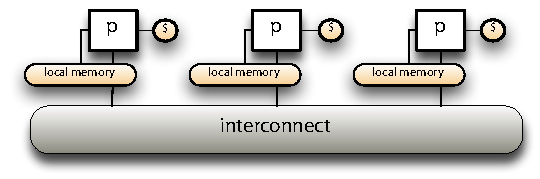
\includegraphics[scale=1.0]{figures/distributed-memory.pdf}
    \end{figure}
    \vspace{-1.0em}
%
    \begin{itemize}
      \item each processor has its own private memory space
      \item processors communicate via the interconnect substrate
    \end{itemize}
%
  \item the programming model
    \begin{itemize}
    \item program consists of a collection of $p$ named processes
      \item each process has its own instruction stream and address space
    \item logically shared data must be partitioned among the processors
    \item communication and synchronization must be orchestrated explicitly 
    \item processes communicate via explicit data exchanges
    \end{itemize}
%
  \end{itemize}
%
\end{frame}

% --------------------------------------
% template
\begin{frame}[fragile]
%
  \frametitle{\mpi\ -- the survivor}
%
  \begin{itemize}
%
  \item the {\em de facto} standard for writing parallel programs using message passing
    \begin{itemize}
    \item a library of routines callable from almost any programming language
    \item that enables communication among multiple processes
    \item standardized and portable API with good implementations available for almost any kind
      of parallel computer
    \end{itemize}
%
  \item \mpi\ is large and complex
    \begin{itemize}
    \item more than 125 functions, lot's of options and communication protocols
    \item but for most practical purposes, a small subset will suffice
    \item short introduction today, more when we consider specific physics
    \end{itemize}
%
  \item two major versions available -- check your installation for compliance
    \begin{itemize}
    \item \mpi-1: parallel machine management, process groups, collective operations,
      point-to-point operations, virtual topologies, profiling
    \item \mpi-2: dynamic process management, one-sided operations, parallel I/O, (simplistic)
      bindings for \cpp
    \end{itemize}
%
  \item \identifier{openmpi}: currently the best open source implementation
    \begin{itemize}
    \item well-architected, thread safe, fast, decent support from a broad community
    \end{itemize}
  \end{itemize}
%
\end{frame}

% --------------------------------------
% compiling, linking, staging and launching
\begin{frame}[fragile]
%
  \frametitle{Getting started}
%
  \begin{itemize}
%
  \item compiling and linking:
    \begin{itemize}
    \item most \mpi\ implementation supply wrappers around the available compilers
      \begin{itemize}
      \item e.g.~\identifier{mpicc}, \identifier{mpic++}, \identifier{mpif77},
        \identifier{mpif90}
      \end{itemize}
    \item it's not magic, so you can do it on your own to
      \begin{itemize}
      \item override the system defaults (without upsetting the sysadmins...)
      \item build multiple versions so you can benchmark
      \end{itemize}
    \end{itemize}
%
  \item staging and launching:
    \begin{itemize}
    \item most implementations provide \identifier{mpirun} to
      \begin{itemize}
      \item control the total number of desired processes
      \item specify the hostnames of the machines to use
      \item specify the mapping of processes to machines/CPUs/cores
      \item establish the current working directory, if possible, for all processes
      \item launch the program
      \end{itemize}
%
    \item but most installations do not permit its use; they have queuing systems instead
      \begin{itemize}
      \item \identifier{PBS}, \identifier{LSF}, \identifier{torque}, \identifier{maui}, ...
      \item specified and documented in the ``welcome'' package of most supercomputer centers
      \item scheduling of jobs, guarantee exclusive access to your allocated machines,
        establish upper time limit, charge the right account for your uses
      \end{itemize}
    \end{itemize}
%
  \end{itemize}
%
\end{frame}

% --------------------------------------
% initializing the runtime environment
\begin{frame}[fragile]
%
  \frametitle{At runtime}
%
  \begin{itemize}
%
%
  \item initializing the co\"operating processes:
    \begin{C}
int MPI_Init(int* argc, char ***argv);
    \end{C}
    \begin{itemize}
    \item note the strange signature; see \slideref{hello-world-mpi} for an example of its use
    \item some implementations -- notably \identifier{MPICH}, the reference implementation --
      used command line arguments to pass information from \identifier{mpirun} to the runtime
      environment
    \item so they need {\em write} access to the command line arguments to strip the extras
    \item thankfully, not done any more
    \end{itemize}
%
  \item must be the first \mpi\ in your program; nothing is initialized correctly until it
    returns
    \begin{itemize}
    \item if this call does not return \identifier{MPI\_SUCCESS}, you should abort
    \end{itemize}
% 
  \item don't forget to shut everything down:
    \begin{C}
int MPI_Finalize(void);
    \end{C}
%
  \item must be the last \mpi\ call in your program; nothing is in usable state after it
    returns
%
  \end{itemize}
%
\end{frame}

% --------------------------------------
% communicators
\begin{frame}[fragile]
%
  \frametitle{Groups and communicators}
%
  \begin{itemize}
%
  \item every \mpi\ process belongs to at least one {\em group}
%
  \item groups have associated {\em communicators} that provide the context for data exchanges and
      synchronization among processes
%
  \item processes in a given communicator get {\em ranked}
    \begin{itemize}
    \item a communicator of $p$ processes assigns ranks 0 through $p-1$
    \item a process can discover the communicator size and its own rank by using
      \begin{C}
int MPI_Comm_size(MPI_Comm communicator, int* size);
int MPI_Comm_rank(MPI_Comm communicator, int* rank);
      \end{C}
    \end{itemize}
% 
  \item the \mpi\ runtime environment creates the {\em global} communicator
    \begin{itemize}
    \item known as \identifier{MPI\_COMM\_WORLD}
    \item all processes are members
    \end{itemize}
% 
  \item it is good practice to learn to manage your own
    \begin{itemize}
    \item to narrow down global operations to processor subsets
    \item to promote {\em reuse}
    \item more details later
    \end{itemize}
% 
  \end{itemize}
%
\end{frame}

% --------------------------------------
% hello world
\begin{frame}[fragile]
%
  \frametitle{Hello world}
%
  \label{slide:hello-world-mpi}
%
  \begin{C}
#include <mpi.h>
#include <stdio.h>

int main(int argc, char* argv[]) {
    int status;
    int rank, size;

    /* initialize MPI */
    status = MPI_Init(&argc, &argv);
    if (status != MPI_SUCCESS) {
        printf("error in MPI_Init; aborting...\n");
        return status;
    }

    /* all good -- get process info and display it */
    MPI_Comm_rank(MPI_COMM_WORLD, &rank);
    MPI_Comm_size(MPI_COMM_WORLD, &size);
    printf("hello from %03d/%03d!\n", rank, size);

    /* shut down MPI */
    MPI_Finalize();

    return 0;
}
  \end{C}
%
\end{frame}

% --------------------------------------
% messages
\begin{frame}[fragile]
%
  \frametitle{Messages}
%
  \begin{itemize}
%
  \item in general, data exchanges through MPI calls involve
    \begin{itemize}
    \item a communicator
      \begin{itemize}
      \item specifies which processes participate in the exchange
      \item resolves process ranks into processes
      \end{itemize}        
    \item {\em collective} operations involve the entire communicator
    \item {\em point-to-point} operations require the rank of the message source or destination
    \item the details of the message payload
      \begin{itemize}
      \item the address of the source buffer
      \item the data type of the buffer contents
      \item the number of items in the buffer
      \end{itemize}
    \end{itemize}
%
    \item \mpi\ provides some data abstractions to
      \begin{itemize}
      \item hide machine dependencies in the data representations to enhance portability and
        support heterogeneous clusters
      \item support user defined data types
      \item support non-contiguous data layouts
      \end{itemize}        
      
%
  \end{itemize}
%
\end{frame}

% --------------------------------------
% global operations
\begin{frame}[fragile]
%
  \frametitle{Collective operations: global reductions}
%
  \begin{itemize}
%
  \item {\em collective} operations involve all processes in a given communicator
%
  \item the \mpi\ version of our global reduction example uses
    \begin{C}
int MPI_Allreduce(
        void* send_buffer, void* recv_buffer,
        int count, MPI_Datatype datatype, MPI_Op operation,
        MPI_Comm communicator
        );
   \end{C}
%
  \item example legal values for \identifier{MPI\_Datatype}
    \begin{itemize}
    \item \cc: \identifier{MPI\_INT}, \identifier{MPI\_LONG}, \identifier{MPI\_DOUBLE} 
    \item \fortran: \identifier{MPI\_INTEGER}, \identifier{MPI\_DOUBLE\_PRECISION},
      \identifier{MPI\_COMPLEX}
    \end{itemize}
%
  \item legal values for \identifier{MPI\_Op}
    \begin{itemize}
    \item \identifier{MPI\_MAX}, \identifier{MPI\_MIN}, \identifier{MPI\_MAXLOC},
      \identifier{MPI\_MINLOC}
    \item \identifier{MPI\_SUM}, \identifier{MPI\_PROD}
    \item \identifier{MPI\_LAND}, \identifier{MPI\_LOR}, \identifier{MPI\_LXOR}
    \item \identifier{MPI\_BAND}, \identifier{MPI\_BOR}, \identifier{MPI\_BXOR}
    \item \identifier{MPI\_REPLACE}
    \end{itemize}
%
  \end{itemize}
%
\end{frame}

% --------------------------------------
% example reduction with mpi
\begin{frame}[fragile]
%
  \frametitle{Example reduction using \mpi}
%
  \label{slide:squares-mpi}
%
  \begin{C}[basicstyle=\tt\bfseries\tiny]
#include <mpi.h>
#include <stdio.h>

int main(int argc, char* argv[]) {
    int status;
    int rank;
    int square, sum;

    /* initialize MPI */
    status = MPI_Init(&argc, &argv);
    if (status != MPI_SUCCESS) {
        printf("error in MPI_Init; aborting...\n");
        return status;
    }

    /* get the process rank */
    MPI_Comm_rank(MPI_COMM_WORLD, &rank);
    /* form the square */
    square = rank*rank;
    /* each process contributes the square of its rank */
    MPI_Allreduce(&square, &sum, 1, MPI_INT,  MPI_SUM, MPI_COMM_WORLD);
    /* print out the result */
    printf("%03d: sum = %d\n", rank, sum);

    /* shut down MPI */
    MPI_Finalize();

    return 0;
}
  \end{C}
%
\end{frame}

% --------------------------------------
% sending and receiving messages
\begin{frame}[fragile]
%
  \frametitle{Point to point communication}
%
  \begin{itemize}
%
  \item to send a message
    \begin{C}
int MPI_Send(
        void* buffer, int count, MPI_Datatype datatype,
        int destination, int tag, MPI_Comm communicator
        );
   \end{C}
%
  \item to receive a message
    \begin{C}
int MPI_Recv(
        void* buffer, int count, MPI_Datatype datatype,
        int source, int tag, MPI_Comm communicator
        );
   \end{C}
%
  \item the \identifier{tag} enables choosing the order you may receive pending messages
%
  \item but for a given (\identifier{source},\identifier{tag},\identifier{communicator})
    messages are received in the order they were sent
%
  \item receiving via wildcards: \identifier{MPI\_ANY\_SOURCE} and \identifier{MPI\_ANY\_TAG}
% 
  \item in {\em standard} communication mode, sending and receiving messages are {\em blocking},
   so the function does not return until you can safely access the \identifier{buffer}
   \begin{itemize}
   \item to read, free, etc.
   \end{itemize}
%
  \end{itemize}
%
\end{frame}

% --------------------------------------
% communication modes
\begin{frame}[fragile]
%
  \frametitle{Communication modes}
%
  \begin{itemize}
%
  \item in standard mode, the specification does not explicitly mention buffering strategy
    \begin{itemize}
    \item buffering messages would remove some of the access constraints but it requires time
      and storage for the multiple copies
    \item portability across implementations implies conservative assumptions about the order
      of initiation of sends and receives to avoid deadlock
    \end{itemize}
%
  \item in {\em ready} mode, you must post a receive before the matching send can be initiated
    \begin{itemize}
    \item \function{MPI\_Rsend}, \function{MPI\_Rrecv}
    \end{itemize}
%
  \item in {\em buffered} mode, sends can be initiated, and may complete, regardless of when
    the matching receive is initiate
    \begin{itemize}
    \item \function{MPI\_Bsend}, \function{MPI\_Brecv}
    \end{itemize}
%
  \item in {\em synchronous} mode, sends can be initiated regardless of whether the matching
    receive has been initiated, but the send will not return until the message has been
    received
    \begin{itemize}
    \item \function{MPI\_Ssend}, \function{MPI\_Srecv}
    \end{itemize}
  \end{itemize}
%
\end{frame}

% --------------------------------------
% asynchronous communications
\begin{frame}[fragile]
%
  \frametitle{Asynchronous communication}
%
  \begin{itemize}
%
  \item there are non-blocking versions of all these
    \begin{C}
int MPI_Isend(
        void* buffer, int count, MPI_Datatype datatype,
        int destination, int tag, 
        MPI_Comm communicator, MPI_Request* request
        );
    \end{C}
    \begin{itemize}
    \item faster, but you must take care to not access the message buffers until the messages
      have been delivered
    \item more details later in the course, as needed
    \end{itemize}
%
  \item for sends
    \begin{itemize}
    \item standard mode: \function{MPI\_Isend}
    \item ready mode: \function{MPI\_Irsend}
    \item buffered mode: \function{MPI\_Ibsend}
    \item synchronous mode: \function{MPI\_Issend}
    \end{itemize}
%
  \item only one call for receives: \function{MPI\_Irecv}
%
  \item extra \identifier{request} argument to check for completion of the request
    \begin{itemize}
    \item \function{MPI\_Test}, \function{MPI\_Wait} and their relatives
    \end{itemize}
%
  \end{itemize}
%
\end{frame}

% --------------------------------------
% creating communicators and groups
\begin{frame}[fragile]
%
  \frametitle{Creating communicators and groups}
%
  \begin{itemize}
%
  \item communicators and groups are intertwined  
    \begin{itemize}
    \item you cannot create a group without a communicator
    \item you cannot create a communicator without a group
    \end{itemize}
%
  \item the cycle is broken by \identifier{MPI\_COMM\_WORLD}
    \begin{C}[basicstyle=\tt\bfseries\tiny]
#include <mpi.h>

int main(int argc, char* argv[]) {
    /* declare a communicator and a couple of groups */
    MPI_Comm workers;
    MPI_Group world_grp, workers_grp;

    /* initialize MPI; for brevity all status checks are omitted */
    MPI_Init(&argc, &argv);

    /* get the world communicator to build its group */
    MPI_Comm_group(MPI_COMM_WORLD, &world_grp);

    /* build another group by excluding a process */
    MPI_Group_excl(world_grp, 1, 0, &workers_grp);

    /* now build a communicator out of the processes in workers_grp */
    MPI_Comm_create(MPI_COMM_WORLD, worker_grp, &workers);

    /* etc.... */

    /* shut down MPI */
    MPI_Finalize();

    return 0;
}
    \end{C}
%
  \end{itemize}
%
\end{frame}

% --------------------------------------
% freeing communicators and groups
\begin{frame}[fragile]
%
  \frametitle{Manipulating communicators and groups}
%
  \begin{itemize}
%
  \item releasing resources
    \begin{C}
int MPI_Group_free(MPI_Group* group);
int MPI_Comm_free(MPI_Comm* communicator);
int MPI_Comm_disconnect(MPI_Comm* communicator);
    \end{C}
%
  \item you can make a new group by adding or removing processes from an existing one
    \begin{C}
int MPI_Group_incl(
    MPI_Group grp, int n, int* ranks, MPI_Group* new_group);
int MPI_Group_excl(
    MPI_Group grp, int n, int* ranks, MPI_Group* new_group);
    \end{C}
%
  \item or by using set operations
    \begin{C}
int MPI_Group_union(
    MPI_Group grp1, MPI_Group grp2, MPI_Group* new_group);
int MPI_Group_intersection(
    MPI_Group grp1, MPI_Group grp2, MPI_Group* new_group);
int MPI_Group_difference(
    MPI_Group grp1, MPI_Group grp2, MPI_Group* new_group);
    \end{C}
%
  \end{itemize}
%
\end{frame}

% --------------------------------------
% virtual topologies
\begin{frame}[fragile]
%
  \frametitle{Virtual topologies}
%
  \begin{itemize}
%
  \item 
%
  \end{itemize}
%
\end{frame}



% --------------------------------------
% timing
\begin{frame}[fragile]
%
  \frametitle{Timing}
%
  \begin{itemize}
%
  \item the function
    \begin{C}
double MPI_Wtime();
    \end{C}
    returns the time in seconds from some arbitrary time in the past
    \begin{itemize}
    \item guaranteed not to change only for the duration of the process
    \end{itemize}
%
  \item you can compute the elapsed time for any program segment by making calls at the
    beginning and the end and computing the difference
%
  \item no guarantees about synchronized clocks among different processes
%
  \item you can compute the clock resolution by using
    \begin{C}
double MPI_Wtick();
    \end{C}
%
  \end{itemize}
%
\end{frame}

% --------------------------------------
% other collective operations
\begin{frame}[fragile]
%
  \frametitle{Other collective operations}
%
  \begin{itemize}
%
  \item \function{MPI\_Scan} computes partial reductions: the \th{p} process receives the
    result from processes 0 through $p-1$
    \begin{C}
int MPI_Scan(
        void* send_buffer, void* recv_buffer,
        int count, MPI_Datatype datatype, MPI_Op operation,
        MPI_Comm communicator
        );
   \end{C}
%
  \item \function{MPI\_Reduce} collects the result at only the given process \identifier{root}
    \begin{C}
int MPI_Reduce(
        void* send_buffer, void* recv_buffer,
        int count, MPI_Datatype datatype, MPI_Op operation,
        int root, MPI_Comm communicator
        );
   \end{C}
%
   \item synchronization is also a global operation:
    \begin{C}
int MPI_Barrier(MPI_Comm communicator);
   \end{C}
%
   participating processes block at a barrier until they have all reached it
%
  \end{itemize}
%
\end{frame}

% --------------------------------------
% scatter
\begin{frame}[fragile]
%
  \frametitle{Scatter}
%
  \begin{itemize}
%
  \item \function{MPI\_Scatter} sends data from \identifier{root} to all processes 
    \begin{C}
int MPI_Scatter(
        void* send_buffer, int send_count, MPI_Datatype send_datatype,
        void* recv_buffer, int recv_count, MPI_Datatype recv_datatype,
        int root, MPI_Comm communicator
        );
    \end{C}
    \begin{figure}
      \centering
      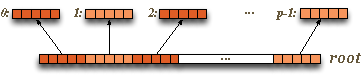
\includegraphics[scale=1.0]{figures/mpi-scatter.pdf}
    \end{figure}
%
  \item it is as if the data in \identifier{send\_buffer} were split in $p$ segments, and the
    \th{i} process receives the \th{i} segment
%
  \item the \identifier{send\_xxx} arguments are only meaningful for \identifier{root}; they
    are ignored for other processes
%
  \item the arguments \identifier{root} and \identifier{communicator} must be passed identical
    values by all processes
%
  \end{itemize}
% 
\end{frame}

% --------------------------------------
% gather
\begin{frame}[fragile]
%
  \frametitle{Gather}
%
  \begin{itemize}
%
  \item the converse is \function{MPI\_Gather} with \identifier{root} receiving data from all
    processes
    \begin{C}
int MPI_Gather(
        void* send_buffer, int send_count, MPI_Datatype send_datatype,
        void* recv_buffer, int recv_count, MPI_Datatype recv_datatype,
        int root, MPI_Comm communicator
        );
   \end{C}
   \begin{figure}
     \centering
     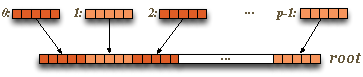
\includegraphics[scale=1.0]{figures/mpi-gather.pdf}
   \end{figure}
%
  \item it is as if $p$ messages, one from each processes, were concatenated in rank order and
    placed at \identifier{recv\_buffer}
%
  \item the \identifier{recv\_xxx} arguments are only meaningful for \identifier{root}; they
    are ignored for other processes
%
  \item the arguments \identifier{root} and \identifier{communicator} must be passed identical
    values by all processes
%
  \end{itemize}
%
\end{frame}

% --------------------------------------
% broadcasts
\begin{frame}[fragile]
%
  \frametitle{Broadcasting operations}
%
  \begin{itemize}
%
  \item \function{MPI\_Alltoall} sends data from all processes to all processes
    \begin{C}
int MPI_Alltoall(
        void* send_buffer, int send_count, MPI_Datatype send_datatype,
        void* recv_buffer, int recv_count, MPI_Datatype recv_datatype,
        MPI_Comm communicator
        );
   \end{C}
%
   a global scatter/gather
%
 \item use \function{MPI\_Bcast} to send the contents of a buffer from \identifier{root} to all
   processes in a communicator
   \begin{C}
int MPI_Bcast(
        void* buffer, int count, MPI_Datatype datatype,
        int root, MPI_Comm communicator
        );
   \end{C}
%
  \end{itemize}
%
\end{frame}

% end of file 

% -*- LaTeX -*-
% -*- coding: utf-8 -*-
%
% ~~~~~~~~~~~~~~~~~~~~~~~~~~~~~~~~~~~~~~~~~~~~~~~~~~~~~~~~~~~~~~~~~~~~~~~~~~~~~~
%
%                             michael a.g. aïvázis
%                      california institute of technology
%                      (c) 1998-2010  all rights reserved
%
% ~~~~~~~~~~~~~~~~~~~~~~~~~~~~~~~~~~~~~~~~~~~~~~~~~~~~~~~~~~~~~~~~~~~~~~~~~~~~~~
%

\pagestyle{headandfoot}
\runningfootrule
\firstpageheader{ACM/CS 114}{Assignment 2}{Due: 27 Jan 2010}
\runningheader{}{}{}
\firstpagefooter{}{}{}
\runningfooter{ACM/CS 114}{Assignment 2}{\thepage}



% --------------------------------------
% reduction using threads
\def\Li{\mbox{\rm Li}_{2}}
\def\len{\mbox{\rm length}}
\def\dilog{\mbox{\tt dilog}}

A better definition for the function $\Li$ is given by
\begin{equation}
\Li(z) \bydef
- \int_{0}^{z} dz' \; \frac{\log(1-z')}{z'} \label{eq:li-def}
\end{equation}
This is well defined for arbitrary complex values $z$, with a branch cut along the real axis
for $z > 1$. It can be shown that
\begin{equation}
  \Li(-1)  = - \frac{\pi^{2}}{12} \label{eq:li-1}
\end{equation}
We will try to establish that \eqref{li-1} is true by numerically evaluating the integral in
\eqref{li-def} {\em in parallel} using both threads and \mpi. Hence, our goal is to show that
\begin{equation}
  \int_{0}^{-1} dz \; \frac{\log(1-z)}{z} = \frac{\pi^{2}}{12} \label{eq:goal} 
\end{equation}
We will employ the following simple numerical integration scheme:
\begin{itemize}
 \item partition the interval $(-1,0)$ into a large number $n$ of subintervals of equal length
 \item evaluate the integrand of \eqref{goal} at the center of each subinterval (why?)
 \item multiply this value by the width of the subinterval to form its contribution to the
   integral
 \item sum up all the contributions
\end{itemize}

\begin{questions}

\question Write a function \function{integrand} that evaluates the integrand of \eqref{goal}
for a given $z$. Assume $z$ is real.

\question Write a function \function{integrator} that implements our integration scheme, given
an interval $(a, b)$ and the desired number of subdivisions $n$.

\question Explain how you would use these two functions to compute an approximation of the
integral in \eqref{goal} {\em in parallel}. In particular, 
\begin{parts}
  \part How would you partition the work into fine grain tasks?
  \part What are the communication requirements among these tasks?
  \part What is the correct coarsening strategy?
  \part How you would map the coarse tasks onto physical processing units?
\end{parts}

\question 

\begin{parts}
  \part Implement this strategy using pthreads.
  \part Implement this strategy using \mpi.
  \part Fill out the following  table
\end{parts}

\end{questions}

% end of file 

% -*- LaTeX -*-
% -*- coding: utf-8 -*-
%
% ~~~~~~~~~~~~~~~~~~~~~~~~~~~~~~~~~~~~~~~~~~~~~~~~~~~~~~~~~~~~~~~~~~~~~~~~~~~~~~
%
%                             michael a.g. aïvázis
%                      california institute of technology
%                      (c) 1998-2010  all rights reserved
%
% ~~~~~~~~~~~~~~~~~~~~~~~~~~~~~~~~~~~~~~~~~~~~~~~~~~~~~~~~~~~~~~~~~~~~~~~~~~~~~~
%

\lecture{Programming GPUs}{20100129}

% --------------------------------------
% template
\begin{frame}[fragile]
%
  \frametitle{Programming GPUs}
%
  \begin{itemize}
%
  \item 
%
  \end{itemize}
%
\end{frame}

% end of file 

% -*- LaTeX -*-
% -*- coding: utf-8 -*-
%
% ~~~~~~~~~~~~~~~~~~~~~~~~~~~~~~~~~~~~~~~~~~~~~~~~~~~~~~~~~~~~~~~~~~~~~~~~~~~~~~
%
%                             michael a.g. aïvázis
%                      california institute of technology
%                      (c) 1998-2010  all rights reserved
%
% ~~~~~~~~~~~~~~~~~~~~~~~~~~~~~~~~~~~~~~~~~~~~~~~~~~~~~~~~~~~~~~~~~~~~~~~~~~~~~~
%

\lecture{A look at parallelism and implementations}{20100201}

% --------------------------------------
% problem statement
\begin{frame}[fragile]
%
  \frametitle{Approximating $\Li$ using a numerical quadrature}
%
  \begin{itemize}
%
  \item the second homework assignment involved $\Li(z)$, defined by
    \begin{equation*}
      \Li(z) \bydef - \int_{0}^{z} dz' \; \frac{\log(1-z')}{z'}
    \end{equation*}
%
    \item the assignment asked for approximating this integral using a simple
      quadrature based on the mid-point rule
      \begin{equation*}
      \Li(z) 
      \approx 
      \Li(z, N) 
      \bydef
      - \frac{z}{N} \sum_{n=0}^{N-1} \left.
        \frac{\log(1-z')}{z'}
      \right|_{z'=(n+\frac{1}{2})\frac{z}{N}}
    \end{equation*}
%
    \item three implementations
      \begin{itemize}
      \item sequential: to get a feeling for how to convert the algorithm into a functioning
        program
      \item parallel using threads: to walk through the parallelization steps and use
        \identifier{pthreads} to get better performance
      \item parallel using \mpi: to get a feel for how \mpi-based programs solve the task
        partitioning problem
      \end{itemize}
%
    \item let's walk through composing, building and running my solutions
      \begin{itemize}
      \item on my desktop, on \href{mind-meld.cacr.caltech.edu}, and on \href{shc.cacr.caltech.edu}
      \end{itemize}
%
  \end{itemize}
%
\end{frame}

% --------------------------------------
% the sequential driver - preamble
\begin{frame}[fragile]
%
  \frametitle{Sequential implementation - part 1}
%
  \begin{itemize}
  \item the preamble
  \begin{lstlisting}[language=c++,name=sequential]
#include <getopt.h> // for getopt and friends
#include <cstdlib>  // for atof
#include <cmath>    // for the correct abs, log

#include <map>
#include <iostream>
#include <iomanip>
  \end{lstlisting}
%
  \item quadrature using the midpoint rule to avoid the singularities
  \begin{lstlisting}[language=c++,name=sequential]
// dilog
double dilog(double z, long N) {
    // initialize
    double dx = z/N;
    double x = dx/2;
    double sum = 0;
    // loop
    for (int i=0; i < N; i++) {
        sum += std::log(1-x)/x;
        x += dx;
    }
    // return; don't forget the sign
    return -dx * sum;
}

  \end{lstlisting}
%
  \end{itemize}
%
\end{frame}

% --------------------------------------
% the sequential driver - the main program
\begin{frame}[fragile]
%
  \frametitle{Sequential implementation - part 2}
%
  \begin{itemize}
  \item using the command line to set $z$ and the number of subdivisions $N$
  \begin{lstlisting}[language=c++,name=sequential]
// main program
int main(int argc, char* argv[]) {
    //  default values for the command line options
    int N = 1000;
    double z = 1.0;

    // read the command line
    int command;
    while ((command = getopt(argc, argv, "z:N:")) != -1) {
        switch (command) {
        // get the argument of the dilogarithm 
        case 'z':
            z = atof(optarg);
            break;
        // get the number of subdivisions
        case 'N':
            N = (int) atof(optarg);
            break;
        }
    }
  \end{lstlisting}
%
  \end{itemize}
%
\end{frame}

% --------------------------------------
% the sequential driver - the main program
\begin{frame}[fragile]
%
  \frametitle{Sequential implementation - part 3}
%
  \begin{itemize}
  \item error checking and computation of the numerical integral
  \begin{lstlisting}[language=c++,name=sequential]
    // error checking
    // abort if N < 1
    if (N < 1) {
        std::cout 
            << "the number of subdivisions must be positive"
            << std::endl;
        return 0;
    }

    // abort for z > 1 to avoid dealing with the imaginary part
    if (z > 1.0) {
        std::cout << "math domain error: z > 1" << std::endl;
        return 0;
    } 

    // compute
    double value = dilog(z, N);
  \end{lstlisting}
%
  \end{itemize}
%
\end{frame}

% --------------------------------------
% the sequential driver - the main program
\begin{frame}[fragile]
%
  \frametitle{Sequential implementation - part 4}
%
  \begin{itemize}
  \item computing the error and printing out the results
  \begin{lstlisting}[language=c++,name=sequential]
    // build a database of the known dilogarithm values
    const double pi = M_PI;
    std::map<double, double> answers;
    answers[1.0] = pi*pi/6;
    answers[-1.0] = -pi*pi/12;

    // print out the value
    std::cout << "Li2(" << z << ")="
        << std::setprecision(17) << std::endl
        << " computed: " << value << std::endl;
    // check whether we know the right answer
    std::map<double,double>::const_iterator lookup = answers.find(z);
    if (lookup != answers.end()) {
        // and if we do, print it out
        double exact = lookup->second;
        std::cout << "    exact: " << exact << std::endl;
        // compute the approximation error and print it out
        double error = std::abs(exact-value)/exact;
        std::cout 
            << std::setiosflags(std::ios_base::scientific) 
            << "    error: " << error << std::endl;
    }

    return 0;
}
  \end{lstlisting}
%
  \end{itemize}
%
\end{frame}

% --------------------------------------
% running the sequential driver
\begin{frame}[fragile]
%
  \frametitle{Building and running the sequential driver}
%
  \begin{shell}{}
#> g++ dilog_sequential.cc -o dilog_sequential
#> dilog_sequential -N 1e7 -z 1.0
Li2(1)=
 computed: 1.6449340282186398
    exact: 1.6449340668482264
    error: 2.34839726522278546e-08
#> time dilog_sequential -N 1e9 -z 1.0
Li2(1)=
 computed: 1.6449339414016682
    exact: 1.6449340668482264
    error: 7.62623625958871898e-08

real    0m19.885s
user    0m19.877s
sys     0m0.003s
#>
  \end{shell}
%
\end{frame}

% --------------------------------------
% the threaded driver - preamble
\begin{frame}[fragile]
%
  \frametitle{Threaded implementation - part 1}
%
  \begin{itemize}
  \item the preamble
  \begin{lstlisting}[language=c++,name=threaded]
#include <getopt.h> // for getopt and friends
#include <pthread.h>

#include <cstdio>
#include <cstdlib>  // for atof
#include <cmath>

#include <map>
#include <iostream>
#include <iomanip>

  \end{lstlisting}
%
  \end{itemize}
%
\end{frame}

% --------------------------------------
% the threaded driver - thread data structures
\begin{frame}[fragile]
%
  \frametitle{Threaded implementation - part 2}
%
  \begin{itemize}
  \item private and shared data structures
  \begin{lstlisting}[language=c++,name=threaded]
// shared information
struct problem {
    int workers;           // total number of threads
    double dz;             // the width of each subdivision
    double sum;            // storage for the partial computations

    pthread_mutex_t lock;  // mutex to control access to the sum
};

// thread specific information
struct context {
    // thread info
    int id;
    pthread_t descriptor;
    // the workload for this thread
    long subdivisions;  // number of subdivisions
    double z_low;       // the lower limit of integration
    double partial;     // record the partial sum computed by this thread
    // the shared problem information
    problem* info;
};
  \end{lstlisting}
%
  \end{itemize}
%
\end{frame}

% --------------------------------------
% the threaded driver - worker
\begin{frame}[fragile]
%
  \frametitle{Threaded implementation - part 3}
%
  \begin{itemize}
  \item the coarse grain task
  \begin{lstlisting}[language=c++,name=threaded]
// worker
void* worker(void* arg) {
    context* ctxt = (context *) arg;
    // pull the problem information from the thread context
    double dz = ctxt->info->dz;
    double z = ctxt->z_low + dz/2;
    // loop over the subdivisions assigned to this thread
    double sum = 0.0;
    for (int i=0; i < ctxt->subdivisions; i++) {
        sum += std::log(1-z)/z;
        z += dz;
    }
    // multiply by the width of each subdivision and adjust the sign
    sum *= -dz;

    // grab the lock
    pthread_mutex_lock(&(ctxt->info->lock));
    // store the result
    ctxt->info->sum += sum;
    // and release the lock
    pthread_mutex_unlock(&(ctxt->info->lock));

    // all done
    return 0;
}
  \end{lstlisting}
%
  \end{itemize}
%
\end{frame}

% --------------------------------------
% the threaded driver - task master
\begin{frame}[fragile]
%
  \frametitle{Threaded implementation - part 4}
%
  \begin{itemize}
  \item the task master -- interface and allocation of storage
  \begin{lstlisting}[language=c++,name=threaded]
// driver
double dilog(double z, long N, int threads) {
    // the width of each interval subdivision
    const double dz = z/N;

    // setup the problem context
    problem info;
    info.workers = threads;
    info.dz = dz;
    info.sum = 0.0;
    pthread_mutex_init(&info.lock, 0);

    // and an array to hold the thread contexts
    context thr_info[threads];
    // partition the number of subdivisions
    long nominal_load = N/threads;

  \end{lstlisting}
%
  \end{itemize}
%
\end{frame}

% --------------------------------------
% the threaded driver - task master continued
\begin{frame}[fragile]
%
  \frametitle{Threaded implementation - part 5}
%
  \begin{itemize}
  \item the task master -- spawning the threads
  \begin{lstlisting}[language=c++,name=threaded]
    // spawn the workers
    for (int tid=0; tid<threads; tid++) {
        // store the thread id
        thr_info[tid].id = tid;
        // point to the shared problem info
        thr_info[tid].info = &info;

        // compute the starting point of the partial integral
        thr_info[tid].z_low = tid*nominal_load*dz;
        // compute the number of subdivisions for this thread
        if (tid == threads - 1) {
            // the last thread gets the leftovers
            thr_info[tid].subdivisions = N - tid*nominal_load;
        } else {
            thr_info[tid].subdivisions = nominal_load;
        }

        // create the thread
        int status = pthread_create(
            &(thr_info[tid].descriptor), 0, worker, &thr_info[tid]);
        if (status) {
            printf("error %d in pthread_create\n", status);
        }
    }
  \end{lstlisting}
%
  \end{itemize}
%
\end{frame}

% --------------------------------------
% the threaded driver - task master continued
\begin{frame}[fragile]
%
  \frametitle{Threaded implementation - part 6}
%
  \begin{itemize}
  \item the task master -- harvesting the threads and returning the result
  \begin{lstlisting}[language=c++,name=threaded]
    // harvest the threads
    for (int tid=0; tid<threads; tid++) {
        pthread_join(thr_info[tid].descriptor, 0);
    }

    // all done
    return info.sum;
}
  \end{lstlisting}
%
  \end{itemize}
%
\end{frame}

% --------------------------------------
% the threaded driver - main program
\begin{frame}[fragile]
%
  \frametitle{Threaded implementation - part 7}
%
  \begin{itemize}
  \item the main program -- reading the command line
  \begin{lstlisting}[language=c++,name=threaded]
// main program
int main(int argc, char* argv[]) {
    //  default values for the command line options
    long N = 1000;
    double z = 1.0;
    int threads = 8;

    // read the command line
    int command;
    while ((command = getopt(argc, argv, "z:N:t:")) != -1) {
        switch (command) {
        case 'z':
            // get the argument of the dilogarithm 
            z = atof(optarg);
            break;
        case 'N':
            // get the number of subdivisions
            N = (long) atof(optarg);
            break;
        case 't':
            // get the numberof threads
            threads = atoi(optarg);
            break;
        }
    }

  \end{lstlisting}
%
  \end{itemize}
%
\end{frame}

% --------------------------------------
% the threaded driver - main program
\begin{frame}[fragile]
%
  \frametitle{Threaded implementation - part 8}
%
  \begin{itemize}
  \item error checking and the invocation of the task master
  \begin{lstlisting}[language=c++,name=threaded]
    // error checking
    // abort if N < 1
    if (N < 1) {
        std::cout 
            << "the number of subdivisions must be positive"
            << std::endl;
        return 0;
    }

    // abort for z > 1 to avoid dealing with the imaginary part
    if (z > 1.0) {
        std::cout << "math domain error: z > 1" << std::endl;
        return 0;
    } 

    // compute
    double value = dilog(z, N, threads);

  \end{lstlisting}
%
  \end{itemize}
%
\end{frame}

% --------------------------------------
% the threaded driver - main program
\begin{frame}[fragile]
%
  \frametitle{Threaded implementation - part 9}
%
  \begin{itemize}
  \item the task master -- printing out the answers
  \begin{lstlisting}[language=c++,name=threaded]
    // build a database of the known dilogarithm values
    const double pi = M_PI;
    std::map<double, double> answers;
    answers[1.0] = pi*pi/6;
    answers[-1.0] = -pi*pi/12;

    // print out the value
    std::cout << "Li2(" << z << ")="
         << std::setprecision(17) << std::endl
         << " computed: " << value << std::endl;
    // check whether we know the right answer
    std::map<double,double>::const_iterator lookup = answers.find(z);
    if (lookup != answers.end()) {
        // and if we do, print it out
        double exact = lookup->second;
        std::cout << "    exact: " << exact << std::endl;
        // compute the approximation error and print it out
        double error = std::abs(exact-value)/exact;
        std::cout 
            << std::setiosflags(std::ios_base::scientific) 
            << "    error: " << error << std::endl;
    }

    return 0;
}
  \end{lstlisting}
%
  \end{itemize}
%
\end{frame}

% --------------------------------------
% running the threaded driver
\begin{frame}[fragile]
%
  \frametitle{Building and running the threaded driver}
%
  \begin{shell}{}
#> g++ dilog_threads.cc -o dilog_threads -pthread
#> dilog_threads -N 1e7 -z 1.0 -t 4
Li2(1)=
 computed: 1.6449340301295035
    exact: 1.6449340668482264
    error: 2.23223068274304058e-08
#> time dilog_threads -N 1e9 -z 1.0 -t 8
Li2(1)=
 computed: 1.6449340044883614
    exact: 1.6449340668482264
    error: 3.79102520315773892e-08

real    0m2.803s
user    0m20.693s
sys     0m0.006s
#>
  \end{shell}
%
\end{frame}

% --------------------------------------
% the mpi driver - the preamble
\begin{frame}[fragile]
%
  \frametitle{MPI implementation - part 1}
%
  \begin{itemize}
  \item the preamble
  \begin{lstlisting}[language=c++,name=mpi]
#include <getopt.h> // for getopt and friends
#include <mpi.h>

#include <cstdio>
#include <cstdlib>  // for atof
#include <cmath>

#include <map>
#include <iostream>
#include <iomanip>

  \end{lstlisting}
%
  \end{itemize}
%
\end{frame}

% --------------------------------------
% the mpi driver -  the coarse grain task
\begin{frame}[fragile]
%
  \frametitle{MPI implementation - part 2}
%
  \begin{itemize}
  \item coarse grain task
  \begin{lstlisting}[language=c++,name=mpi]
double dilog(double zprime, long N, int id, int processes) {
    // the width of each interval subdivision
    const double dz = zprime/N;
    // compute the starting point of the partial integral
    const double z_low = id*zprime/processes;
    // partition the number of subdivisions
    long nominal_load = N/processes;
    // the last process gets the leftovers
    if (id == processes - 1) {
        nominal_load = N - id*nominal_load;
    }
    // initialize the partial sum
    double sum = 0.0;
    double z = z_low + dz/2;
    // loop over the subdivisions assigned to this thread
    for (int i=0; i < nominal_load; i++)  {
        sum += std::log(1-z)/z;
        z += dz;
    }
    // collect the partial answers from all the processes
    double value;
    MPI_Allreduce(
        &sum, &value, 1, MPI_DOUBLE, MPI_SUM, MPI_COMM_WORLD);
    // multiply by the width of each subdivision and adjust the sign
    return -dz*value;
}
  \end{lstlisting}
%
  \end{itemize}
%
\end{frame}

% --------------------------------------
% the mpi driver - the main program
\begin{frame}[fragile]
%
  \frametitle{MPI implementation - part 3}
%
  \begin{itemize}
  \item the main program -- setting up \mpi
  \begin{lstlisting}[language=c++,name=mpi]
// main program
int main(int argc, char* argv[]) {
    // initialize MPI
    int status = MPI_Init(&argc, &argv);
    if (status != MPI_SUCCESS) {
        std::cout << "error in MPI_Init; aborting..." << std::endl;
        return status;
    }
    // get process information from the world communicator
    int id, processes;
    MPI_Comm_rank(MPI_COMM_WORLD, &id);
    MPI_Comm_size(MPI_COMM_WORLD, &processes);

  \end{lstlisting}
%
  \end{itemize}
%
\end{frame}

% --------------------------------------
% the mpi driver - the main program
\begin{frame}[fragile]
%
  \frametitle{MPI implementation - part 4}
%
  \begin{itemize}
  \item reading the command line
  \begin{lstlisting}[language=c++,name=mpi]
    //  default values for the command line options
    long N = 1000;
    double z = 1.0;
    // read the command line
    int command;
    while ((command = getopt(argc, argv, "z:N:")) != -1) {
        switch (command) {
        case 'z':
            // get the argument of the dilogarithm 
            z = atof(optarg);
            break;
        case 'N':
            // get the number of subdivisions
            N = (long) atof(optarg);
            break;
        }
    }
  \end{lstlisting}
%
  \end{itemize}
%
\end{frame}

% --------------------------------------
% the mpi driver -  error checking and computation
\begin{frame}[fragile]
%
  \frametitle{MPI implementation - part 5}
%
  \begin{itemize}
  \item error checking and computation
  \begin{lstlisting}[language=c++,name=mpi]
    // error checking
    // abort if N < 1
    if (N < 1) {
        if (id == 0) {
            std::cout 
                << "the number of subdivisions must be positive"
                << std::endl;
        }
        MPI_Finalize();
        return 0;
    }
    // abort for z > 1 to avoid dealing with the imaginary part
    if (z > 1.0) {
        if (id == 0) {
            std::cout << "math domain error: z > 1" << std::endl;
        }
        MPI_Finalize();
        return 0;
    } 
    // compute
    double value = dilog(z, N, id, processes);
    if (id != 0) { // let all but processor 0 die
        // shut down MPI
        MPI_Finalize();
        return 0;
    }
  \end{lstlisting}
%
  \end{itemize}
%
\end{frame}

% --------------------------------------
% the mpi driver - printing out the results
\begin{frame}[fragile]
%
  \frametitle{MPI implementation - part 6}
%
  \begin{itemize}
  \item printing out the results
  \begin{lstlisting}[language=c++,name=mpi]
    // build a database of the known dilogarithm values
    const double pi = M_PI;
    std::map<double, double> answers;
    answers[1.0] = pi*pi/6;
    answers[-1.0] = -pi*pi/12;

    // print out the value
    std::cout << "Li2(" << z << ")=" << std::setprecision(17) << std::endl;
    std::cout << " computed: " << value << std::endl;
    // check whether we know the right answer
    std::map<double,double>::const_iterator lookup = answers.find(z);
    if (lookup != answers.end()) {
        // and if we do, print it out
        double exact = lookup->second;
        std::cout << "    exact: " << exact << std::endl;
        // compute the approximation error and print it out
        double error = std::abs(exact-value)/exact;
        std::cout 
            << std::setiosflags(std::ios_base::scientific) 
            << "    error: " << error << std::endl;
    }

    // shut down MPI
    MPI_Finalize();
    return 0;
}
  \end{lstlisting}
%
  \end{itemize}
%
\end{frame}

% --------------------------------------
% running the mpi driver
\begin{frame}[fragile]
%
  \frametitle{Building and running the \mpi\ driver}
%
  \begin{itemize}
  \item on my desktop, or \href{mind-meld.cacr.caltech.edu}
    \begin{itemize}
    \item where there is no queue manager
    \end{itemize}
  \end{itemize}
%
  \begin{shell}{}
#> mpic++ dilog_mpi.cc -o dilog_mpi -lmpi_cxx -lmpi
#> mpirun -np 4 dilog_mpi -N 1e7 -z 1.0
Li2(1)=
 computed: 1.6449340301295035
    exact: 1.6449340668482264
    error: 2.23223068274304058e-08
#> time mpirun -np 8 dilog_mpi -N 1e9 -z 1.0
Li2(1)=
 computed: 1.6449340044883614
    exact: 1.6449340668482264
    error: 3.79102520315773892e-08

real    0m3.697s
user    0m0.018s
sys     0m0.015s
#>
  \end{shell}
%
\end{frame}

% --------------------------------------
% running the mpi driver
\begin{frame}[fragile]
%
  \frametitle{Running the \mpi\ driver on a shared resource}
%
  \begin{itemize}
  \item on \href{shc.cacr.caltech.edu} there is a queue manager
    \begin{itemize}
    \item don't use \identifier{mpirun}: you are running on the head node
    \item instead, request a dedicated node
    \end{itemize}
  \end{itemize}
%
  \begin{shell}{}
# shc-a> mpic++ dilog_mpi.cc -o dilog_mpi
# shc-a> qsub -I -l nodes=1:core8 -l walltime=0:15:00
qsub: waiting for job 105059.mistress to start
qsub: job 105059.mistress ready
Logging in as aivazis on shc168, a Linux-2.x_x86_64 system
  setting up: (environment) (aliases) (machines) (tools: Linux-2.x_x86_64)
# shc168> time mpirun -np 8 dilog_mpi -N 1e9 -z 1.0
Li2(1)=
 computed: 1.6449340044883614
    exact: 1.6449340668482264
    error: 3.79102520315773892e-08

real    0m10.501s
user    1m14.642s
sys     0m0.273s
# shc168> exit
logout
qsub: job 105059.mistress completed
# shc-a>
  \end{shell}
%
\end{frame}

% end of file 

% -*- LaTeX -*-
% -*- coding: utf-8 -*-
%
% ~~~~~~~~~~~~~~~~~~~~~~~~~~~~~~~~~~~~~~~~~~~~~~~~~~~~~~~~~~~~~~~~~~~~~~~~~~~~~~
%
%                             michael a.g. aïvázis
%                      california institute of technology
%                      (c) 1998-2010  all rights reserved
%
% ~~~~~~~~~~~~~~~~~~~~~~~~~~~~~~~~~~~~~~~~~~~~~~~~~~~~~~~~~~~~~~~~~~~~~~~~~~~~~~
%

\lecture{Functional decomposition}{20100203}

% --------------------------------------
% functional decomposition
\begin{frame}[fragile]
%
  \frametitle{Functional decomposition}
%
  \begin{itemize}
%
  \item {\em functional decomposition} determines the fine grain parallel tasks by partitioning
    the problem into semi-independent tasks that can be executed in parallel
%
  \item our numerical integration examples fall in this category
    \begin{itemize}
    \item partitioning identified the finest grain work unit as the evaluation of the
      integrand; no need for fancy domain decomposition
    \item little or no communication/synchronization is required among the tasks, i.e. the are
      embarrassingly parallel
    \item coarsening consists of grouping fine grain tasks into larger work units in a straight
      forward manner
    \item the mapping of the coarse grain tasks onto processing units is trivial
    \end{itemize}
%
  \item in general, the computations involved in carrying out the coarse tasks are
    computationally equivalent
    \begin{itemize}
    \item the computation is {\em self balancing}
    \item or there is no need for sophisticated load balancing
    \end{itemize}
%
  \item scalability and parallel efficiency are determined by the particulars of the problem,
    such as inherent limitations on the largest problem size of interest
%
  \end{itemize}
%
\end{frame}

% --------------------------------------
% relevant problems
\begin{frame}[fragile]
%
  \frametitle{Blank}
%
  \begin{itemize}
%
  \item a variety of interesting problems can be cast in this form
%
  \end{itemize}
%
\end{frame}


% end of file 

% -*- LaTeX -*-
% -*- coding: utf-8 -*-
%
% ~~~~~~~~~~~~~~~~~~~~~~~~~~~~~~~~~~~~~~~~~~~~~~~~~~~~~~~~~~~~~~~~~~~~~~~~~~~~~~
%
%                             michael a.g. aïvázis
%                      california institute of technology
%                      (c) 1998-2010  all rights reserved
%
% ~~~~~~~~~~~~~~~~~~~~~~~~~~~~~~~~~~~~~~~~~~~~~~~~~~~~~~~~~~~~~~~~~~~~~~~~~~~~~~
%

\lecture{Optimization}{20100205}

% --------------------------------------
% the problem in general
\begin{frame}[fragile]
%
  \frametitle{Optimization}
%
  \begin{itemize}
%
  \item broadly speaking, given a function $f$ and a region $\Omega$ in its domain,
    optimization seeks an $x \in \Omega$ such that $f(x)$ is an extremum; we write
    \begin{equation}
      \optimum{\Omega} f
    \end{equation}
% 
    \item $f$ is often referred to as the {\em objective function}, $\Omega$ is known as {\em
        configuration space}, and the $x \in \Omega$ are called {\em configurations}; other
      names may be common in your field
%
    \item typically only interested in maxima or minima
%
    \item the configuration space $\Omega$ is an essential part of the problem
      \begin{itemize}
      \item may be specified in terms of {\em constraints} satisfied by allowable
        configurations
      \end{itemize}
%
  \item if $f$ is not convex, there may be more than one local extremum; {\em global
      optimization} is the study of algorithms that converge to the actual extremum in finite
    time.
%
  \end{itemize}
%
\end{frame}

% --------------------------------------
% parallel optimization
\begin{frame}[fragile]
%
  \frametitle{Parallel optimization}
%
  \begin{itemize}
%
  \item sources of potential parallelism
    \begin{itemize}
    \item exploration of the configuration space
    \item evaluation of $f$
    \end{itemize}
%
  \end{itemize}
%
\end{frame}


% --------------------------------------
% quasi-newton
\begin{frame}[fragile]
%
  \frametitle{Overview of quasi-Newton}
%
  \begin{itemize}
%
    \item family of methods use the Taylor expansion of $f$ about an iterate $x$ to construct a
      quadratic local approximation and use the first and second derivatives to find the
      stationary point
%
    \item the Taylor expansion yields
      \begin{equation}
        f(x+dx) 
        \approx 
        f(x) 
        + (\partial_{i} f) dx^{i} 
        + \frac{1}{2} dx^{i} (\partial_{ij} f) dx^{j}
    \end{equation}
    in terms of the gradient $\partial_{i} f$ and the Hessian $\partial_{ij} f$ about the
    iterate $x$
% 
  \item differentiate and set to 0 to provide the update step
    \begin{equation}
      \partial_{i} f + (\partial_{ij} f) dx^{j} \approx 0
    \end{equation}
    by inverting the Hessian
%
    \item the distinguishing features among members of this family are the way $(\partial_{ij}
      f)$ is approximated since the secant equation
      \begin{equation}
        \partial_{i} f(x+dx) = \partial_{i} f(x) + (\partial_{ij} f(x)) dx^{j}
      \end{equation}
      is not enough to constrain it fully in more than one dimension
% 
  \end{itemize}
% 
\end{frame}

% --------------------------------------
% simulated annealing
\begin{frame}[fragile]
%
  \frametitle{Simulated annealing}
%
  \begin{itemize}
  \item 
  \end{itemize}
%
\end{frame}


% --------------------------------------
% genetic algorithms
\begin{frame}[fragile]
%
  \frametitle{Genetic algorithms}
%
  \begin{itemize}
  \item 
  \end{itemize}
%
\end{frame}


% end of file 

% -*- LaTeX -*-
% -*- coding: utf-8 -*-
%
% ~~~~~~~~~~~~~~~~~~~~~~~~~~~~~~~~~~~~~~~~~~~~~~~~~~~~~~~~~~~~~~~~~~~~~~~~~~~~~~
%
%                             michael a.g. aïvázis
%                      california institute of technology
%                      (c) 1998-2010  all rights reserved
%
% ~~~~~~~~~~~~~~~~~~~~~~~~~~~~~~~~~~~~~~~~~~~~~~~~~~~~~~~~~~~~~~~~~~~~~~~~~~~~~~
%

\lecture{Overview}{20100208}

% --------------------------------------
% Overview
\begin{frame}[fragile]
%
  \frametitle{Overview}
%
  \begin{itemize}
%
  \item
% 
  \end{itemize}
%
\end{frame}

% end of file 

% -*- LaTeX -*-
% -*- coding: utf-8 -*-
%
% ~~~~~~~~~~~~~~~~~~~~~~~~~~~~~~~~~~~~~~~~~~~~~~~~~~~~~~~~~~~~~~~~~~~~~~~~~~~~~~
%
%                             michael a.g. aïvázis
%                      california institute of technology
%                      (c) 1998-2010  all rights reserved
%
% ~~~~~~~~~~~~~~~~~~~~~~~~~~~~~~~~~~~~~~~~~~~~~~~~~~~~~~~~~~~~~~~~~~~~~~~~~~~~~~
%

\lecture{Structured grids - II}{20100210}

% --------------------------------------
% sequential
\begin{frame}[fragile]
%
  \frametitle{Sequential implementation - the preamble}
%
  \begin{itemize}
  \item back up to the beginning of the file
    \begin{lstlisting}[language=c++,name=seq:frame, firstnumber=1]
#include <getopt.h>
#include <cmath>
#include <cstdlib>
#include <fstream>
#include <iostream>

// forward declarations
class Grid;
class Visualizer;

// the solver; does nothing for the time being
void initialize(Grid & grid) {};
void laplace(Grid & grid, double tolerance){};

    \end{lstlisting}
%
  \item we have separated out {\em visualization} in a different object to support different
    formats without disturbing the data representation
%
  \item \identifier{initialize} and \identifier{laplace} have trivial implementations for now
    \begin{itemize}
    \item enables testing the scaffolding without worrying about the solver
      implementation just yet
    \end{itemize}
  \end{itemize}
% 
\end{frame}

% --------------------------------------
% sequential
\begin{frame}[fragile]
%
  \frametitle{Sequential implementation - the grid object stub}
%
  \begin{lstlisting}[language=c++,name=seq:frame]
// the solution representation
class Grid {
    // interface: TBD
public:

    // meta methods
public:
    Grid(size_t size);
    ~Grid();

    // private data members: TBD
private:

    // disabled interface
    // grid will own dynamic memory, so don't let the compiler screw up
private:
    Grid(const Grid &);
    const Grid & operator= (const Grid &);
};

// the grid implementation
Grid::Grid(size_t size) {
}

Grid::~Grid() {
}

  \end{lstlisting}
% 
\end{frame}

% --------------------------------------
% sequential
\begin{frame}[fragile]
%
  \frametitle{Sequential implementation - the visualizer stub}
%
  \begin{lstlisting}[language=c++,name=seq:frame, firstnumber=1]
// the visualizer class
class Visualizer {
    // local type aliases
public:
    typedef std::ostream stream_t;

    // interface
public:
    void csv(const Grid & grid, stream_t & stream);

    // meta methods
public:
    inline Visualizer() {}
};

// the Visualizer class implementation
void Visualizer::csv(const Grid & grid, Visualizer::stream_t & stream) {
    return;
}
  \end{lstlisting}
%

\begin{itemize}
\item the code now compiles and links
  \begin{itemize}
  \item consistency check that the object collaborations are ok, for now
  \item can be tested for command line option parsing
  \end{itemize}
\end{itemize}
% 
\end{frame}

% --------------------------------------
% the grid initializer
\begin{frame}[fragile]
%
  \frametitle{Fleshing out the initializer}
%
  \begin{lstlisting}[language=c++,name=seq:initializer]
// the grid initializer:
// zero out and apply our boundary conditions 
void initialize(Grid & grid) {
    // ask the grid to clear its memory
    grid.clear(1.0);
    // apply the dirichlet conditions
    for (size_t cell=0; cell < grid.size(); cell++) {
        // evaluate sin(pi x)
        double sin = std::sin(cell * grid.delta() * pi);
        // along the x axis, at top and  bottom
        grid(cell, 0) = sin;
        grid(cell, grid.size()-1) = sin * std::exp(-pi);
        // along the y axis, left and right
        grid(0, cell) = 0.0;
        grid(grid.size()-1, cell) = 0.0;
    }

    return;
}
  \end{lstlisting}
%
  \begin{itemize}
  \item the grid knows its size, its spacing $\delta$, and can zero out its  memory
  \item access to grid elements happens through an overloaded \identifier{operator()} so we can
    {\em encapsulate} the indexing function
  \end{itemize}
%
\end{frame}

% --------------------------------------
% the grid declaration
\begin{frame}[fragile]
%
  \frametitle{The grid class declaration}
%
  \begin{lstlisting}[language=c++,name=seq:grid]
// the solution representation
class Grid {
    // interface
public:
    // zero out all cells
    void clear(double value=0.0);
    // the grid dimensions
    size_t size() const {return _size;}
    // the grid spacing
    double delta() const {return _delta;}
    // access to the cells
    double & operator()(size_t i, size_t j) {return _block[j*_size+i];}
    double operator()(size_t i, size_t j) const {return _block[j*_size+i];}
    // meta methods
public:
    Grid(size_t size);
    ~Grid();
    // data members
private:
    const size_t _size;
    const double _delta;
    double* _block;
    // disable these
private:
    Grid(const Grid &);
    const Grid & operator= (const Grid &);
};
  \end{lstlisting}
%
\end{frame}

% --------------------------------------
% the grid implementation
\begin{frame}[fragile]
%
  \frametitle{The grid class implementation}
%
  \begin{lstlisting}[language=c++,name=seq:grid]
// the grid implementation
// interface
void Grid::clear(double value) {
    for (size_t i=0; i < _size*_size; i++) {
        _block[i] = value;
    }

    return;
}

// constructor
Grid::Grid(size_t size) :
    _size(size), 
    _delta((1.0 - 0.0)/(size-1)),
    _block(new double[size*size]) {
}

// destructor
Grid::~Grid() {
    delete [] _block;
}

  \end{lstlisting}
%
\end{frame}

% --------------------------------------
% the grid visualizer
\begin{frame}[fragile]
%
  \frametitle{Grid visualization}
%
  \begin{lstlisting}[language=c++,name=seq:visualizer]
// the visualizer class
class Visualizer {
    // local type aliases
public:
    typedef std::ostream stream_t;
    // interface
public:
    void csv(const Grid & grid, stream_t & stream);
    // meta methods
public:
    inline Visualizer() {}
};

// the Visualizer class implementation
void Visualizer::csv(const Grid & grid, Visualizer::stream_t & stream) {
    for (size_t j=0; j < grid.size(); j++) {
        stream << j;
        for (size_t i=0; i < grid.size(); i++) {
            stream << "," << grid(i,j);
        }
        stream << std::endl;
    }

    return;
}

  \end{lstlisting}
%
\end{frame}

% --------------------------------------
% the results of initialization
\begin{frame}[fragile]
%
  \frametitle{Printing out the initial grid}
%
  \begin{itemize}
  \item we should be able to print out the initialized grid
  \end{itemize}
%
  \begin{shell}{}
#> mm laplace
#> laplace
#> cat laplace.csv
0,0,0.3827,0.7071,0.9239,1,0.9239,0.7071,0.3827,1.225e-16
1,0,1,1,1,1,1,1,1,0
2,0,1,1,1,1,1,1,1,0
3,0,1,1,1,1,1,1,1,0
4,0,1,1,1,1,1,1,1,0
5,0,1,1,1,1,1,1,1,0
6,0,1,1,1,1,1,1,1,0
7,0,1,1,1,1,1,1,1,0
8,0,0.01654,0.0306,0.03992,0.04321,0.0399,0.03056,0.01654,0
  \end{shell}
%
\end{frame}

% --------------------------------------
% the solver
\begin{frame}[fragile]
%
  \frametitle{Fleshing out the solver}
%
  \begin{lstlisting}[language=c++,basicstyle=\tt\bfseries\tiny,name=seq:solver]
// the solver driver
void laplace(Grid & current, double tolerance) {
    // create and initialize temporary storage
    Grid next(current.size());
    initialize(next);
    // put an upper bound on the number of iterations
    long max_iterations = (long) (1./tolerance);
    for (long iterations = 0; iterations<max_iterations; iterations++) {
        double max_dev = 0.0;
        // do an iteration step
        // leave the boundary alone
        // iterate over the interior of the grid
        for (size_t j=1; j < current.size()-1; j++) {
            for (size_t i=1; i < current.size()-1; i++) {
                // update
                next(i,j) = 0.25*(
                    current(i+1,j)+current(i-1,j)+current(i,j+1)+current(i,j-1));
                // compute the deviation from the last generation
                double dev = std::abs(next(i,j) - current(i,j));
                // and update the maximum deviation
                if (dev > max_dev) {
                    max_dev = dev;
                }
            }
        }
        // swap the blocks between the two grids
        Grid::swapBlocks(current, next);
        // check covergence
        if (max_dev < tolerance) {
            break;
        }
    }
    return;
}
  \end{lstlisting}
%
\end{frame}

% end of file 

% -*- LaTeX -*-
% -*- coding: utf-8 -*-
%
% ~~~~~~~~~~~~~~~~~~~~~~~~~~~~~~~~~~~~~~~~~~~~~~~~~~~~~~~~~~~~~~~~~~~~~~~~~~~~~~
%
%                             michael a.g. aïvázis
%                      california institute of technology
%                      (c) 1998-2010  all rights reserved
%
% ~~~~~~~~~~~~~~~~~~~~~~~~~~~~~~~~~~~~~~~~~~~~~~~~~~~~~~~~~~~~~~~~~~~~~~~~~~~~~~
%

\lecture{Structured grids - III}{20100212}

% --------------------------------------
% the results of initialization
\begin{frame}[fragile]
%
  \frametitle{Printing out the initial grid}
%
  \begin{itemize}
  \item we should be able to print out the initialized grid
%
  \begin{shell}{}
#> mm laplace
#> laplace
#> cat laplace.csv
0,0,0.3827,0.7071,0.9239,1,0.9239,0.7071,0.3827,1.225e-16
1,0,1,1,1,1,1,1,1,0
2,0,1,1,1,1,1,1,1,0
3,0,1,1,1,1,1,1,1,0
4,0,1,1,1,1,1,1,1,0
5,0,1,1,1,1,1,1,1,0
6,0,1,1,1,1,1,1,1,0
7,0,1,1,1,1,1,1,1,0
8,0,0.01654,0.0306,0.03992,0.04321,0.0399,0.03056,0.01654,0
  \end{shell}
%
  \item notice that
    \begin{itemize}
    \item the top line contains some recognizable values
    \item the left and right borders are set to zero
    \item the interior of the grid is painted with our initial guess
    \end{itemize}
%
  \item still to do:
    \begin{itemize}
    \item write the update
    \item build a grid with the exact solution 
    \item build the error field (why?)
    \end{itemize}
  \end{itemize}
%
\end{frame}

% --------------------------------------
% the solver
\begin{frame}[fragile]
%
  \frametitle{Fleshing out the solver}
%
  \begin{lstlisting}[language=c++,basicstyle=\tt\bfseries\tiny,name=seq:solver,firstnumber=169]
// the solver driver
void laplace(Grid & current, double tolerance) {
    // create and initialize temporary storage
    Grid next(current.size());
    initialize(next);
    // put an upper bound on the number of iterations
    long max_iterations = (long) 1e4;;
    for (long iterations = 0; iterations<max_iterations; iterations++) {
        double max_dev = 0.0;
        // do an iteration step
        // leave the boundary alone
        // iterate over the interior of the grid
        for (size_t j=1; j < current.size()-1; j++) {
            for (size_t i=1; i < current.size()-1; i++) {
                // update
                next(i,j) = 0.25*(
                    current(i+1,j)+current(i-1,j)+current(i,j+1)+current(i,j-1));
                // compute the deviation from the last generation
                double dev = std::abs(next(i,j) - current(i,j));
                // and update the maximum deviation
                if (dev > max_dev) {
                    max_dev = dev;
                }
            }
        }
        // swap the blocks between the two grids
        Grid::swapBlocks(current, next);
        // check covergence
        if (max_dev < tolerance) {
            break;
        }
    }
    return;
}
  \end{lstlisting}
%
\end{frame}

% --------------------------------------
% the updated grid class
\begin{frame}[fragile]
%
  \frametitle{Adding the new grid interface}
%
  \begin{itemize}
  \item here is the declaration of \function{Grid::swapBlocks}
%
    \begin{lstlisting}[language=c++,firstnumber=30]
class Grid {
    // interface
    public:
    ...
    // exchange the data blocks of two compatible grids
    static void swapBlocks(Grid &, Grid &);
    ...
};
    \end{lstlisting}
%
  \item and its definition
%
    \begin{lstlisting}[language=c++,firstnumber=69]
void Grid::swapBlocks(Grid & g1, Grid & g2) {
    // bail out if the two operands are not compatible
    if (g1.size() != g2.size()) {
        throw "Grid::swapblocks: size mismatch";
    }
    if (g1.delta() != g2.delta()) {
        throw "Grid::swapblocks: spacing mismatch";
    }
    // but if they are, just exhange their data buffers
    double * temp = g1._block;
    g1._block = g2._block;
    g2._block = temp;
    // all done
    return;
}
    \end{lstlisting}
%
  \end{itemize}
%
\end{frame}

% --------------------------------------
% rework the driver to print out the exact solution and the error field
\begin{frame}[fragile]
%
  \frametitle{Reworking the driver}
%
  \begin{lstlisting}[language=c++,basicstyle=\tt\bfseries\tiny,name=seq:driver,firstnumber=239]
    // build a visualizer
    Visualizer vis;

    // compute the exact solution
    Grid solution(N);
    exact(solution);
    std::fstream exact_stream("exact.csv", std::ios_base::out);
    vis.csv(solution, exact_stream);
    
    // allocate space for the solution
    Grid potential(N);
    // initialize and apply our boundary conditions
    initialize(potential);
    // call the solver
    laplace(potential, tolerance);
    // open a stream to hold the answer
    std::fstream output_stream(filename, std::ios_base::out);
    // build a visualizer and render the solution in our chosen format
    vis.csv(potential, output_stream);

    // compute the error field
    Grid error(N);
    relative_error(potential, solution, error);
    std::fstream error_stream("error.csv", std::ios_base::out);
    vis.csv(error, error_stream);

    // all done
    return 0;
}
  \end{lstlisting}
%
\end{frame}

% --------------------------------------
% computing the exact and error fields
\begin{frame}[fragile]
% 
  \frametitle{Computing the exact solution and the error field}
%
  \begin{lstlisting}[language=c++,firstnumber=143]
void exact(Grid & grid) {
    //  paint the exact solution
    for (size_t j=0; j < grid.size(); j++) {
        for (size_t i=0; i < grid.size(); i++) {
            double x = i*grid.delta();
            double y = j*grid.delta();
            grid(i,j) = std::exp(-pi*y)*std::sin(pi*x);
        }
    }
    return;
}

void relative_error(
    const Grid & computed, const Grid & exact, Grid & error) {
    //  compute the relative error
    for (size_t j=0; j < exact.size(); j++) {
        for (size_t i=0; i < exact.size(); i++) {
            if (exact(i,j) == 0.0) { // hm... sloppy!
                error(i,j) = std::abs(computed(i,j));
            } else {
                error(i,j) = std::abs(computed(i,j) - exact(i,j))/exact(i,j);
            }
        }
    }
    return;
}

  \end{lstlisting}
%
\end{frame}

% --------------------------------------
% assessment
\begin{frame}[fragile]
%
  \frametitle{Shortcomings}
%
  \begin{itemize}
%
  \item numerics:
    \begin{itemize}
    \item it converges very slowly; other update {\em schemes} improve on this
    \item our approximation is very low order, so it takes very large grids to produce a few
      digits of accuracy
    \item the convergence criterion has some unwanted properties; it triggers
      \begin{itemize}
      \item prematurely: large swaths of constant values may never get updated
      \item it would trigger even if we were updating the wrong grid!
      \end{itemize}
    \end{itemize}
%
  \item design:
    \begin{itemize}
    \item separate the problem specification from its solution
    \item there are other objects lurking, waiting to be uncovered
    \item someone should make the graphic visualizer
    \item restarts anybody?
    \item how would you try out different convergence criteria? update schemes? memory layouts?
    \end{itemize}
%
    \item usability:
      \begin{itemize}
      \item supporting interchangeable parts requires damage to the top level driver
        \begin{itemize}
        \item to enable the user to make the selection
        \item to expose new command line arguments that configure the new parts
        \end{itemize}
      \end{itemize}
%
  \end{itemize}
%
\end{frame}

% --------------------------------------
% assessment
\begin{frame}[fragile]
%
  \frametitle{Assessing our fundamental}
%
  \begin{itemize}
%
  \item \class{Grid} is a good starting point for abstracting structured grids
    \begin{itemize}
    \item assumes ownership of the memory associated with a structured grid
    \item encapsulates the indexing function
    \item extend it to
      \begin{itemize}
      \item support different memory layout strategies
      \item support non-square grids (?)
      \item support non-uniform grids (?)
      \item higher dimensions
      \item if you need any of these, consider using one of the many excellent class libraries
        written by experts
      \end{itemize}
    \end{itemize}
%
  \item \class{Visualizer}, under another name, can form the basis for a more general
    persistence library
    \begin{itemize}
    \item to support HDF5, NetCDF, bitmaps, voxels, etc.
    \end{itemize}
%
  \end{itemize}
%
\end{frame}

% --------------------------------------
% the Problem class
\begin{frame}[fragile]
% 
  \frametitle{The \class{Problem} class: the interface}
%
  \begin{lstlisting}[language=c++,name=Problem]
// the solution representation
class acm114::laplace::Problem {
    //typedefs
public:
    typedef std::string string_t;
    // interface
public:
    inline string_t name() const;
    inline const Grid & exact() const;
    inline const Grid & deviation() const;
    inline Grid & solution();
    inline const Grid & solution() const;
    inline Grid & error();
    inline const Grid & error() const;
    // abstract
    virtual void initialize() = 0;
    virtual void initialize(Grid &) const = 0;
    // meta methods
public:
    inline Problem(string_t name, double width, size_t points);
    virtual ~Problem();
    // data members
  \end{lstlisting}
%
\end{frame}

% --------------------------------------
% the Problem class
\begin{frame}[fragile]
% 
  \frametitle{The \class{Problem} class: the data}
%
  \begin{lstlisting}[language=c++,name=Problem]
protected:
    string_t _name;
    double _delta;
    Grid _solution;
    Grid _exact;
    Grid _error;
    Grid _deviation;
    // disable these
private:
    Problem(const Problem &);
    const Problem & operator= (const Problem &);
};
  \end{lstlisting}
%
\end{frame}

% --------------------------------------
% our specific example
\begin{frame}[fragile]
% 
  \frametitle{The \class{Example} class}
%
  \begin{lstlisting}[language=c++]
class acm114::laplace::Example : public acm114::laplace::Problem {
    // interface
public:
    virtual void initialize();
    virtual void initialize(Grid &) const;

    // meta methods
public:
    inline Example(string_t name, double width, size_t points);
    virtual ~Example();

    // disable these
private:
    Example(const Example &);
    const Example & operator= (const Example &);
};

  \end{lstlisting}
%
\end{frame}

% --------------------------------------
% the solver basis
\begin{frame}[fragile]
% 
  \frametitle{The \class{Solver} class}
%
  \begin{lstlisting}[language=c++]
class acm114::laplace::Solver {
    // interface
public:
    virtual void solve(Problem &) = 0;

    // meta methods
public:
    inline Solver();
    virtual ~Solver();

    // data members
private:

    // disable these
private:
    Solver(const Solver &);
    const Solver & operator= (const Solver &);
};

  \end{lstlisting}
%
\end{frame}

% --------------------------------------
% the jacobi solver 
\begin{frame}[fragile]
% 
  \frametitle{The \class{Jacobi} class}
%
  \begin{lstlisting}[language=c++]
class acm114::laplace::Jacobi : public acm114::laplace::Solver {
    // interface
public:
    virtual void solve(Problem &);

    // meta methods
public:
    inline Jacobi(double tolerance, size_t workers);
    virtual ~Jacobi();

    // implementation details
protected:
    virtual void _solve(Problem &);
    static void * _update(void *);

    // data members
private:
    double _tolerance;
    size_t _workers;

    // disable these
private:
    Jacobi(const Jacobi &);
    const Jacobi & operator= (const Jacobi &);
};

  \end{lstlisting}
%
\end{frame}

% end of file 

% -*- LaTeX -*-
% -*- coding: utf-8 -*-
%
% ~~~~~~~~~~~~~~~~~~~~~~~~~~~~~~~~~~~~~~~~~~~~~~~~~~~~~~~~~~~~~~~~~~~~~~~~~~~~~~
%
%                             michael a.g. aïvázis
%                      california institute of technology
%                      (c) 1998-2010  all rights reserved
%
% ~~~~~~~~~~~~~~~~~~~~~~~~~~~~~~~~~~~~~~~~~~~~~~~~~~~~~~~~~~~~~~~~~~~~~~~~~~~~~~
%

\lecture{Structured grids - parallelization with threads}{20100217}

% --------------------------------------
% parallelization using threads
\begin{frame}[fragile]
%
  \frametitle{Parallelization using threads}
%
  \begin{itemize}
%
  \item the shared memory implementation requires
    \begin{itemize}
    \item a scheme so that threads can update cells without the need for locks
    \item while maximizing locality of data access
    \item even the computation of the convergence criterion can be parallelized
    \end{itemize}
%
  \item parallelization strategy
    \begin{itemize}
    \item we will focus on parallelizing the iterative grid update
      \begin{itemize}
      \item grid initialization, visualization, computing the exact answer and the error field
        do not depend on the {\em number of iterations}
      \end{itemize}
    \item the finest grain of work is clearly an individual cell update based on the value of
      its four nearest neighbors
    \item for this two dimensional example, we can build coarser grain tasks using
      \begin{itemize}
      \item horizontal or vertical strips
      \item non-overlapping blocks
      \item the strategy gets more complicated if you want to perform the update in place
      \end{itemize}
    \item the communication patterns are trivial for the double buffering layout; only the
      final update of the convergence criterion requires any locking
    \item each coarse grain task can be assigned to a thread
    \end{itemize}
%
  \end{itemize}
% 
\end{frame}

% --------------------------------------
% required changes to the sequential driver
\begin{frame}[fragile]
%
  \frametitle{Required changes to the sequential solution}
%
  \begin{itemize}
%
  \item what is needed
    \begin{itemize}
    \item an object to hold the problem information shared among the threads
    \item the per-thread administrative data structure that holds the thread id and the pointer
      to the shared information
      \begin{itemize}
      \item this is the argument to \function{pthread\_create}
      \end{itemize}
    \item a mutex to protect the update of the global convergence criterion
    \item a \function{pthread\_create} compatible worker routine
    \item a change at the top-level driver to enable the user to choose the number of threads
    \end{itemize}
%
  \item and a strategy for managing the thread life cycle
    \begin{itemize}
%
    \item synchronization is trivial if
      \begin{itemize}
      \item we spawn our threads to perform the updates of a single iteration
      \item harvest them
      \item check the convergence criterion 
      \item stop, or respawn them if another iteration is necessary
      \end{itemize}
%
    \item can the convergence test be done in parallel?
      \begin{itemize}
        \item so we don't have to pay the create/harvest overhead?
        \item if so, how do we guarantee correctness and consistency?
      \end{itemize}
%
    \end{itemize}
% 
  \end{itemize}
%
\end{frame}

% --------------------------------------
% the jacobi solver 
\begin{frame}[fragile]
% 
  \frametitle{Threaded \class{Jacobi}: thread data}
%
  \begin{lstlisting}[language=c++,name=Jacobi:threaded]
struct Task {
    // shared information 
    size_t workers;
    Grid & current;
    Grid & next;
    double maxDeviation;
    // mutex to control access to the convergence criterion
    pthread_mutex_t lock; 

    Task(size_t workers, Grid & current, Grid & next) :
        workers(workers), current(current), next(next), maxDeviation(0.0) {
        pthread_mutex_init(&lock, 0);
    }
};

struct Context {
    // thread info
    size_t id;
    pthread_t descriptor;
    Task * task;
};

  \end{lstlisting}
%
\end{frame}

% --------------------------------------
% the jacobi solver 
\begin{frame}[fragile]
% 
  \frametitle{Threaded \class{Jacobi}: driving the update}
%
  \begin{lstlisting}[language=c++,name=Jacobi:threaded]
void Jacobi::solve(Problem & problem) {
    // initialize the problem
    problem.initialize();
    // do the actual solve
    _solve(problem);
    // compute and store the error
    std::cout << "  computing absolute error" << std::endl;
    //  compute the relative error
    Grid & error = problem.error();
    const Grid & exact = problem.exact();
    const Grid & solution = problem.solution();

    for (size_t j=0; j < exact.size(); j++) {
        for (size_t i=0; i < exact.size(); i++) {
            if (exact(i,j) == 0.0) {
                error(i,j) = std::abs(solution(i,j));
            } else {
                error(i,j) = std::abs(solution(i,j) - exact(i,j))/exact(i,j);
            }
        }
    }
    std::cout << " --- done." << std::endl;
    return;
}
  \end{lstlisting}
%
\end{frame}

% --------------------------------------
% the jacobi solver 
\begin{frame}[fragile]
% 
  \frametitle{Threaded \class{Jacobi}: the master thread}
%
  \begin{lstlisting}[language=c++,name=Jacobi:threaded]
void Jacobi::_solve(Problem & problem) {
    Grid & current = problem.solution();

    // create and initialize temporary storage
    Grid next(current.size());
    problem.initialize(next);

    // shared thread info
    Task task(_workers, current, next);
    // per-thread information
    Context context[_workers];

    // let's get going
    std::cout << "jacobi: tolerance=" << _tolerance << std::endl;

    // put an upper bound on the number of iterations
    const size_t max_iterations = (size_t) 1.0e4;
  \end{lstlisting}
%
\end{frame}

% --------------------------------------
% the jacobi solver 
\begin{frame}[fragile]
% 
  \frametitle{Threaded \class{Jacobi}: the master thread, part 2}
%
  \begin{lstlisting}[language=c++,name=Jacobi:threaded,basicstyle=\tt\bfseries\tiny]
    for (size_t iterations = 0; iterations<max_iterations; iterations++) {
        if (iterations % 100 == 0) {
            std::cout << "     " << iterations << std::endl;
        }
        // reset the maximium deviation
        task.maxDeviation = 0.0;
        // spawn the threads
        for (size_t tid=0; tid < _workers; tid++) {
            context[tid].id = tid;
            context[tid].task = &task;

            int status = pthread_create(&context[tid].descriptor, 0, _update, &context[tid]);
            if (status) {
                throw ("error in pthread_create");
            }
        }
        // harvest the threads
        for (size_t tid = 0; tid < _workers; tid++) {
            pthread_join(context[tid].descriptor, 0);
        }

        // swap the blocks between the two grids
        Grid::swapBlocks(current, next);
        // check covergence
        if (task.maxDeviation < _tolerance) {
            std::cout << " ### convergence in " << iterations << " iterations!" << std::endl;
            break;
        }
    }
    std::cout << " --- done." << std::endl;

    return;
}
  \end{lstlisting}
%
\end{frame}

% --------------------------------------
% the jacobi solver 
\begin{frame}[fragile]
% 
  \frametitle{Threaded \class{Jacobi}: update in the worker threads}
%
  \begin{lstlisting}[language=c++,basicstyle=\tt\bfseries\tiny,name=Jacobi:threaded]
void * Jacobi::_update(void * arg) {
    Context * context = static_cast<Context *>(arg);

    size_t id = context->id;
    Task * task = context->task;

    size_t workers = task->workers;
    Grid & current = task->current;
    Grid & next = task->next;
    pthread_mutex_t lock = task->lock;

    double max_dev = 0.0;
    // do an iteration step
    // leave the boundary alone
    // iterate over the interior of the grid
    for (size_t j=id+1; j < current.size()-1; j+=workers) {
        for (size_t i=1; i < current.size()-1; i++) {
            next(i,j) = 0.25*(current(i+1,j)+current(i-1,j)+current(i,j+1)+current(i,j-1));
            // compute the deviation from the last generation
            double dev = std::abs(next(i,j) - current(i,j));
            // and update the maximum deviation
            if (dev > max_dev) {
                max_dev = dev;
            }
        }
    }

    // grab the lock and update the global maximum deviation
    pthread_mutex_lock(&lock);
    if (task->maxDeviation < max_dev) {
        task->maxDeviation = max_dev;
    }
    pthread_mutex_unlock(&lock);

    return 0;
}
  \end{lstlisting}
%
\end{frame}

% --------------------------------------
% improving the threaded implementation
\begin{frame}[fragile]
%
  \frametitle{Assessing the threaded implementation}
%
  \begin{itemize}
%
  \item the implemented synchronization scheme is very simple
    \begin{itemize}
    \item each grid update step spawns some number of workers to update a subset of the cells
    \item the workers are harvested after the grid is updated
    \item the main thread checks for convergence
    \item if another iteration is required, a new set of workers is spawned
    \end{itemize}
%
  \item the simplicity of this strategy comes at a cost
    \begin{itemize}
    \item {\em scalability} suffers when the overhead of creating and harvesting threads is
      comparable to amount of work done by each thread
    \item for low thread counts, it is still an overall win, since the time to solution
      decreases and the machine utilization is better
    \item but as the number of threads increases, the program becomes {\em slower}
      \begin{itemize}
      \item timing a $100\times100$ grid to convergence on a recent MacPro
%
        \begin{equation*}
          \begin{array}{r|ccccc}
% header
            {\rm threads } & 1 & 2 & 4 & 8 & 16 \\
            \hline 
            {\rm time} (s) & 4.367 & 2.517 & 1.918 & 1.937 & 3.537
% 
          \end{array}
        \end{equation*}
      \item and 10,000 iterations of a $1000\times1000$ grid
        \begin{equation*}
          \begin{array}{r|ccccc}
% header
            {\rm threads } & 1 & 2 & 4 & 8 & 16 \\
            \hline 
            {\rm time} (s) & 413.306 & 211.050 & 109.509 & 98.279 & 74.087
% 
          \end{array}
        \end{equation*}
      \end{itemize}

    \end{itemize}
%
\end{itemize}
%
\end{frame}

% --------------------------------------
% template
\begin{frame}[fragile]
%
  \frametitle{Improving the update loop}
%
  \begin{itemize}
%
  \item the plan is to keep the workers alive and updating the grid while either we converge or
    \identifier{max\_iterations} is reached
  \item the main thread
    \begin{itemize}
    \item spawns all the threads
    \item enters a loop to count the number of iterations completed
    \item grabs a job control mutex
    \item blocks until all the threads have finished updating their sections of the grid
    \item checks the stopping criteria and sets a flag to indicate whether we are done
    \item release the job control mutex 
    \item if done, iterate
    \item otherwise, exit the loop and harvest the threads
    \end{itemize}
%
  \end{itemize}
%
\end{frame}

% end of file 

% -*- LaTeX -*-
% -*- coding: utf-8 -*-
%
% ~~~~~~~~~~~~~~~~~~~~~~~~~~~~~~~~~~~~~~~~~~~~~~~~~~~~~~~~~~~~~~~~~~~~~~~~~~~~~~
%
%                             michael a.g. aïvázis
%                      california institute of technology
%                      (c) 1998-2010  all rights reserved
%
% ~~~~~~~~~~~~~~~~~~~~~~~~~~~~~~~~~~~~~~~~~~~~~~~~~~~~~~~~~~~~~~~~~~~~~~~~~~~~~~
%

\lecture{Structured grids - parallelization with threads}{20100217}

% --------------------------------------
% Improving the update loop
\begin{frame}[fragile]
%
  \frametitle{Improving the update loop}
%
  \begin{itemize}
%
  \item the plan is to keep the workers alive and updating the grid while either we converge or
    \identifier{max\_iterations} is reached
  \item the main thread
    \begin{itemize}
    \item loops to spawn all the threads
    \item and immediately enters a loop to harvest them
    \end{itemize}
%
  \item the workers use a condition variable to synchronize among themselves
    \begin{itemize}
    \item they iterate, updating the grid
    \item grab a mutex, deposit their local maximum deviation from the last iterations, update
      a counter that records how many workers have completed their update, and release the lock
    \item enter another critical section with the termination logic
      \begin{itemize}
      \item everybody uses a condition variable to wait for the slowest worker
      \item the slowest worker checks the convergence criterion and updates the termination
        flag, swaps the grid blocks and signals everybody else
      \item if the termination flag is set, or if the maximum number of iterations has been
        reached, all threads exit
      \end{itemize}
    \end{itemize}
%
  \end{itemize}
%
\end{frame}

% --------------------------------------
% the jacobi solver 
\begin{frame}[fragile]
% 
  \frametitle{Threaded \class{Jacobi}: the main thread}
%
  \begin{lstlisting}[language=c++,name=Jacobi:updated-solve,basicstyle=\tt\bfseries\tiny]
void Jacobi::_solve(Problem & problem) {
    Grid & current = problem.solution();

    // create and initialize temporary storage
    Grid next(current.size());
    problem.initialize(next);

    // shared thread info
    Task task(_workers, _tolerance, current, next);
    // per-thread information
    Context context[_workers];
    // spawn the threads
    std::cout << "jacobi: spawning " << _workers << " workers" << std::endl;
    for (size_t tid=0; tid < _workers; tid++) {
        context[tid].id = tid;
        context[tid].task = &task;
        
        int status = pthread_create(&context[tid].descriptor, 0, _update, &context[tid]);
        if (status) {
            throw ("error in pthread_create");
        }
    }
    // harvest the threads
    for (size_t tid = 0; tid < _workers; tid++) {
            pthread_join(context[tid].descriptor, 0);
        }
    // done
    std::cout << "jacobi: done." << std::endl;
    return;
}
  \end{lstlisting}
%
\end{frame}

% --------------------------------------
% the jacobi solver 
\begin{frame}[fragile]
% 
  \frametitle{Threaded \class{Jacobi}: updated thread data}
%
  \begin{lstlisting}[language=c++,name=Jacobi:updated-threaded,basicstyle=\tt\bfseries\tiny]
struct Task {
    // shared information 
    size_t workers; // the number of threads
    double tolerance; // the covergence tolerance
    Grid & current;
    Grid & next;

    bool done; // is there more work?
    double maxDeviation; // the value
    size_t contributions; // the number of threads that have deposited contributions
    pthread_mutex_t gridUpdate_lock; //the mutex
    pthread_cond_t gridUpdate_check;

    Task(size_t workers, double tolerance, Grid & current, Grid & next) :
        workers(workers), tolerance(tolerance), current(current), next(next),
        done(false), maxDeviation(0.0), contributions(0),
        gridUpdate_lock(), gridUpdate_check() {
        // initialize the grid update lock
        pthread_mutex_init(&gridUpdate_lock, 0);
        pthread_cond_init(&gridUpdate_check, 0);
    }

    ~Task() {
        pthread_mutex_destroy(&gridUpdate_lock);
        pthread_cond_destroy(&gridUpdate_check);
    }
};

  \end{lstlisting}
%
\end{frame}

% --------------------------------------
% the jacobi solver 
\begin{frame}[fragile]
% 
  \frametitle{Threaded \class{Jacobi}: workers, part 1}
%
  \begin{lstlisting}[language=c++,name=Jacobi:updated-solve,basicstyle=\tt\bfseries\tiny]
// the threaded update
void * Jacobi::_update(void * arg) {
    Context * context = static_cast<Context *>(arg);

    size_t id = context->id;
    Task * task = context->task;

    const size_t workers = task->workers;
    Grid & current = task->current;
    Grid & next = task->next;

    size_t maxIterations = (size_t) 1e4;
    // iterate, updating the grid until done
    for (size_t iteration = 0; iteration < maxIterations; iteration++) {
        // thread 0: print an update
        if (id == 0 && iteration % 100 == 0) {
            std::cout << "    " << iteration << std::endl;
        }

        double max_dev = 0.0;
        // do an iteration step
        // leave the boundary alone
        // iterate over the interior of the grid
        for (size_t j=id+1; j < current.size()-1; j+=workers) {
            for (size_t i=1; i < current.size()-1; i++) {
                next(i,j) = 0.25*(current(i+1,j)+current(i-1,j)+current(i,j+1)+current(i,j-1));
                // compute the deviation from the last generation
                double dev = std::abs(next(i,j) - current(i,j));
                // and update the maximum deviation
                if (dev > max_dev) {
                    max_dev = dev;
                }
            }
        }
        // done with the grid update
  \end{lstlisting}
%
\end{frame}

% --------------------------------------
% the jacobi solver 
\begin{frame}[fragile]
% 
  \frametitle{Threaded \class{Jacobi}: workers, part 2}
%
  \begin{lstlisting}[language=c++,name=Jacobi:updated-solve,basicstyle=\tt\bfseries\tiny]
        // grab the grid update lock
        pthread_mutex_lock(&task->gridUpdate_lock);
        // update the global maximum deviation 
        if (task->maxDeviation < max_dev) {
            task->maxDeviation = max_dev;
        }
        // leave a mark
        task->contributions++;
        // bookkeeping at the end of the  update
        if (task->contributions == workers) {
            // if i am the slowest worker
            // swap the blocks between the two grids
            Grid::swapBlocks(current, next);
            // check covergence
            if (task->maxDeviation < task->tolerance) {
                std::cout
                    << " +++ thread " << id << ": convergence in " << iteration << " iterations"
                    <<std::endl;
                task->done = true;
            }
            // reset our accounting and signal everybody
            task->contributions = 0;
            task->maxDeviation = 0;
            pthread_cond_broadcast(&task->gridUpdate_check);
        } else {
            // all but the slowest wait here
            pthread_cond_wait(&task->gridUpdate_check, &task->gridUpdate_lock);
        } 
        // release
        pthread_mutex_unlock(&task->gridUpdate_lock);
        // check whether we are done
        if (task->done) {
            break;
        }
    }
    return 0;
}
  \end{lstlisting}
%
\end{frame}

% --------------------------------------
% improving the threaded implementation
\begin{frame}[fragile]
%
  \frametitle{Assessing the improved implementation}
%
  \begin{itemize}
%
  \item the improved threading scheme is not much more complex
    \begin{itemize}
    \item we keep track of how many threads have computed their grid update
    \item the slowest worker check the convergence criterion and performs all the necessary
      bookkeeping 
    \item while everybody else waits
    \item use \function{pthread\_cond\_brodacast} to wake the other workers
    \end{itemize}
%
  \item here is the performance comparison for 10,000 iterations on a $1000 \times 1000$ grid
    on the same 8-core MacPro
    \begin{equation*}
      \begin{array}{r|ccccc}
% header
        {\rm threads } & 1 & 2 & 4 & 8 & 16 \\
        \hline 
        {\rm previous} (s) & 413.306 & 211.050 & 109.509 & 98.279 & 74.087 \\
        {\rm updated} (s)  & 408.636 & 208.832 & 107.015 & 59.043 & 61.481 \\
% 
      \end{array}
    \end{equation*}
%
  \end{itemize}
%
\end{frame}

% --------------------------------------
% parallelization with MPI
\begin{frame}[fragile]
%
  \frametitle{Parallelization with \mpi}
%
  \begin{itemize}
%
  \item the \mpi\ implementation will require careful data management
    \begin{itemize}
    \item we must partition the mesh among processes
    \item each process work on its own subgrid
      \begin{itemize}
      \item it will allocate its own memory, for both actual data and the guard zones
      \item it must locate its patch in physical space
      \end{itemize}
    \item communication is required every iteration
      \begin{itemize}
      \item so that neighbors can synchronize their boundaries
      \item think of the synchronization as a kind of boundary condition!
      \end{itemize}
    \item parallel convergence testing involves a collective operation
    \end{itemize}
%
  \end{itemize}
%
  \begin{figure}
    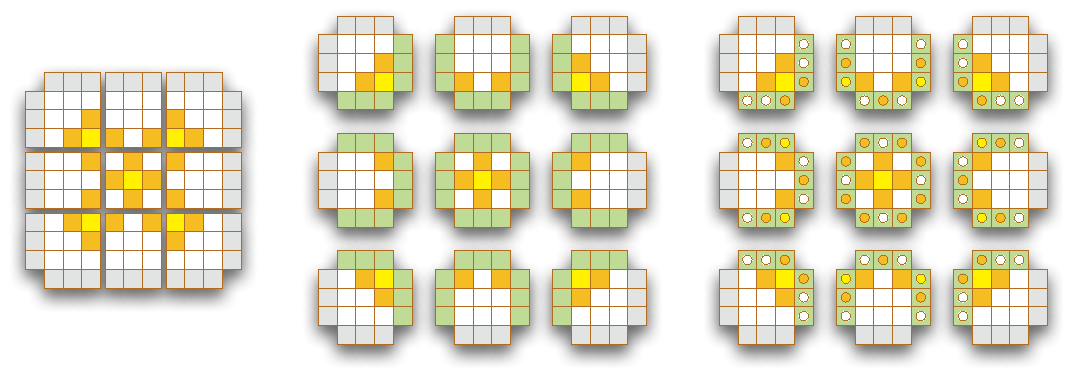
\includegraphics[scale=0.5]{figures/structured-partitioning.pdf}
  \end{figure} 
% 
\end{frame}

% --------------------------------------
% template
\begin{frame}[fragile]
%
  \frametitle{A little bit of help}
%
  \begin{itemize}
%
  \item \mpi\ supports this common use case through a Cartesian {\em virtual topology}
    \begin{itemize}
    \item a special communicator with a map from a $d$-dimensional virtual process grid to the
      normal linear process ranks
    \item and local operations that enable you to discover the ranks of your virtual neighbors
    \item there is even a special form of send/receive so that you don't have to worry about
      contention and race conditions during the boundary synchronization
    \end{itemize}
%
  \item to create a Cartesian communicator
    \begin{C}
int MPI_Cart_create(MPI_Comm oldcomm,
        int ndims, int* layout, int* periods, int reorder, MPI_Comm* newcomm);
    \end{C}
%
  \item to find out the coordinates of a process in the virtual grid given its rank
    \begin{C}
int MPI_Cart_coords(MPI_Comm cartesian,
        int rank, int ndims, int* coords); 
    \end{C}
%
    \item you can also find out the ranks of your neighbors
    \begin{C}
int MPI_Cart_shift(MPI_Comm cartesian,
        int dimension, int shift, int* origin, int* neighbor); 
    \end{C}
%
  \end{itemize}
%
\end{frame}

% --------------------------------------
% the mpi driver
\begin{frame}[fragile]
%
  \frametitle{The \mpi\ driver, part 1}
%
  \begin{lstlisting}[language=c++,name=mpi:driver,firstnumber=26,basicstyle=\tt\bfseries\tiny]
int main(int argc, char* argv[]) {
    int status;
    // initialize mpi
    status = MPI_Init(&argc, &argv);
    if (status) {
        throw("error in MPI_Init");
    }
    // get my rank in the world communicator
    int worldRank, worldSize;
    MPI_Comm_rank(MPI_COMM_WORLD, &worldRank);
    MPI_Comm_size(MPI_COMM_WORLD, &worldSize);
    size_t processors = static_cast<size_t>(std::sqrt(worldSize));

    // default values for our user configurable settings
    size_t n = 9; // points per processor
    size_t threads = 1;
    double tolerance = 1.0e-3;

    // read the command line
    int command;
    while ((command = getopt(argc, argv, "n:e:t:")) != -1) {
        switch (command) {
        // get the convergence tolerance
        case 'e':
            tolerance = atof(optarg);
            break;
        // get the grid size
        case 'n':
            n = (size_t) atof(optarg);
            break;
        // get the number of threads
        case 't':
            threads = (size_t) atoi(optarg);
            break;
        }
    }
  \end{lstlisting}
% 
\end{frame}

% --------------------------------------
% the mpi driver
\begin{frame}[fragile]
%
  \frametitle{The \mpi\ driver, part 2}
%
  \begin{lstlisting}[language=c++,name=mpi:driver,basicstyle=\tt\bfseries\tiny]
    // print out the chosen options
    if (worldRank == 0) {
        for (int arg = 0; arg < argc; ++arg) {
            std::cout << argv[arg] << " ";
        }
        std::cout
            << std::endl
            << "    grid size: " << n << std::endl
            << "      workers: " << threads << std::endl
            << "    tolerance: " << tolerance << std::endl;
    }

    // instantiate a problem
    Example problem("cliche", 1.0, processors, n);

    // instantiate a solver
    Jacobi solver(tolerance, threads);
    // solve
    solver.solve(problem);
    // save the results
    Visualizer vis;
    vis.csv(problem);

    // initialize mpi
    status = MPI_Finalize();
    if (status) {
        throw("error in MPI_Finalize");
    }

    // all done
    return 0;
}
  \end{lstlisting}
% 
\end{frame}

% --------------------------------------
% the mpi driver
\begin{frame}[fragile]
%
  \frametitle{The \class{Jacobi} declaration}
%
  \begin{lstlisting}[language=c++,name=mpi:jacobi-decl,basicstyle=\tt\bfseries\tiny]
class acm114::laplace::Jacobi : public acm114::laplace::Solver {
    // interface
public:
    virtual void solve(Problem &);

    // meta methods
public:
    inline Jacobi(double tolerance, size_t workers);
    virtual ~Jacobi();

    // data members
private:
    double _tolerance;
    size_t _workers;

    // disable these
private:
    Jacobi(const Jacobi &);
    const Jacobi & operator= (const Jacobi &);
};
  \end{lstlisting}
% 
\end{frame}

% --------------------------------------
% the problem base class
\begin{frame}[fragile]
%
  \frametitle{The \class{Problem} declaration}
%
  \begin{lstlisting}[language=c++,name=mpi:problem-decl,basicstyle=\tt\bfseries\tiny]
class acm114::laplace::Problem {
    //typedefs
public:
    typedef std::string string_t;
    // interface
public:
    string_t name() const;
    inline MPI_Comm communicator() const;
    inline int rank() const;
    // access to my grid
    inline Grid & solution();
    inline const Grid & solution() const;
    // interface used by the solver
    virtual void initialize();
    virtual void applyBoundaryConditions() = 0;
    // meta methods
public:
    Problem(string_t name, double interval, int processors, size_t points);
    virtual ~Problem();
    // data members
protected:
    string_t _name;
    double _delta, _x0, _y0;
    int _rank, _size, _processors;
    int _place[2];
    MPI_Comm _cartesian;
    Grid _solution;
    // disable these
private:
    Problem(const Problem &);
    const Problem & operator= (const Problem &);
};
  \end{lstlisting}
% 
\end{frame}

% --------------------------------------
% problem definitions
\begin{frame}[fragile]
%
  \frametitle{The \class{Problem} constructor}
%
  \begin{lstlisting}[language=c++,name=mpi:driver,basicstyle=\tt\bfseries\tiny]
Problem::Problem(
    string_t name, double interval, int processors, size_t points) :
    _name(name),
    _delta(interval/((points-2)*processors+1)),
    _x0(0.0), _y0(0.0),
    _rank(0), _size(0), _processors(processors), _place(),
    _cartesian(),
    _solution(points) {

    // build the intended layout
    int layout[] = { processors, processors };
    // find my rank in the world communicator
    int worldRank;
    MPI_Comm_rank(MPI_COMM_WORLD, &worldRank);
    // build a Cartesian communicator
    int periods[] = { 0, 0 };
    MPI_Cart_create(MPI_COMM_WORLD, 2, &layout[0], periods, 1, &_cartesian);
    // check whether i can paritcipate
    if (_cartesian != MPI_COMM_NULL) {
        // get my rank in the cartesian communicator
        MPI_Comm_rank(_cartesian, &_rank);
        MPI_Comm_size(_cartesian, &_size);
        // get my logical position on the process grid
        MPI_Cart_coords(_cartesian, _rank, 2, &_place[0]);
        // now compute my offset in physical space
        _x0 = 0.0 + (points-2)*_place[0]*_delta;
        _y0 = 0.0 + (points-2)*_place[1]*_delta;
    } else {
        // i was left out because the total number of processors is not a square
        std::cout
            << "world rank " << worldRank << ": not a member of the cartesian communicator "
            << std::endl;
    }
}
  \end{lstlisting}
% 
\end{frame}


% --------------------------------------
% the Example declaration
\begin{frame}[fragile]
%
  \frametitle{The \class{Example} declaration}
%
  \begin{lstlisting}[language=c++,name=mpi:example-decl]
class acm114::laplace::Example : public acm114::laplace::Problem {
    // interface
public:
    virtual void applyBoundaryConditions();

    // meta methods
public:
    inline Example(
        string_t name, double interval, int processors, size_t points);
    virtual ~Example();

    // disable these
private:
    Example(const Example &);
    const Example & operator= (const Example &);
};
  \end{lstlisting}
% 
\end{frame}

% --------------------------------------
% the solver
\begin{frame}[fragile]
%
  \frametitle{The implementation of \method{Jacobi::solve}, part 1}
%
  \begin{lstlisting}[language=c++,name=mpi:solver,fistnumber=14,basicstyle=\tt\bfseries\tiny]
void Jacobi::solve(Problem & problem) {
    // initialize the problem
    problem.initialize();

    // get a reference to the solution grid
    Grid & current = problem.solution();
    // build temporary storage for the next iterant
    Grid next(current.size());

    // put an upper limit on the number of iterations
    size_t maxIterations = (size_t) 1e4;
    for (size_t iteration = 0; iteration < maxIterations; iteration++) {
        // print out a progress repot
        if ((problem.rank() == 0) && (iteration % 100 == 0)) {
            std::cout 
                << "jacobi: iteration " << iteration
                << std::endl;
        }
        // enforce  the boundary conditions
        problem.applyBoundaryConditions();
        // reset the local maximum change
        double localMax = 0.0;
        // update the interior of the grid
        for (size_t j=1; j < next.size()-1; j++) {
            for (size_t i=1; i < next.size()-1; i++) {
                // the cell update
                next(i,j) = .25*(current(i+1,j)+current(i-1,j)+current(i,j+1)+current(i,j-1));
                // compute the change from the current cell value
                double dev = std::abs(next(i,j) - current(i,j));
                // and update the local maximum
                if (dev > localMax) {
                    localMax = dev;
                }
            }
        } // done with the grid update
  \end{lstlisting}
% 
\end{frame}

% --------------------------------------
% the solver driver
\begin{frame}[fragile]
%
  \frametitle{The implementation of \method{Jacobi::solve}, part 2}
%
  \begin{lstlisting}[language=c++,name=mpi:solver,basicstyle=\tt\bfseries\tiny]
        // swap the blocks of the two grids, leaving the solution in current
        Grid::swapBlocks(current, next);
        // compute global maximum deviation
        double globalMax;
        MPI_Allreduce(&localMax, &globalMax, 1, MPI_DOUBLE, MPI_MAX, problem.communicator());
        // convergence check
        if (globalMax < _tolerance) {
            if (problem.rank() == 0) {
                std::cout 
                    << "jacobi: convergence in " << iteration << " iterations"
                    << std::endl;
            }
            break;
        }
        // otherwise
    }
    // when we get here, either we have converged or ran out of iterations
    // update the fringe of the current grid
    problem.applyBoundaryConditions();
    // all  done
    return;
}
  \end{lstlisting}
% 
\end{frame}

% --------------------------------------
% applying boundary conditions
\begin{frame}[fragile]
%
  \frametitle{Boundary conditions and data exchanges, part 1}
%
  \begin{lstlisting}[language=c++,name=mpi:example-impl]
void Example::applyBoundaryConditions() {
    // a reference to my grid
    Grid & g = _solution;
    // my rank;
    int rank = _rank;
    // the ranks of my four neighbors
    int top, right, bottom, left;
    // get them
    MPI_Cart_shift(_cartesian, 1, 1, &rank, &top);
    MPI_Cart_shift(_cartesian, 0, 1, &rank, &right);
    MPI_Cart_shift(_cartesian, 1, -1, &rank, &bottom);
    MPI_Cart_shift(_cartesian, 0, -1, &rank, &left);

    // allocate send and receive buffers
    double * sendbuf = new double[g.size()];
    double * recvbuf = new double[g.size()];
  \end{lstlisting}
% 
\end{frame}

% --------------------------------------
% applying boundary conditions
\begin{frame}[fragile]
%
  \frametitle{Boundary conditions and data exchanges, part 2}
%
  \begin{lstlisting}[language=c++,name=mpi:example-impl]
    // shift to the right
    // fill my sendbuf with my RIGHT DATA BORDER
    for (size_t cell=0; cell < g.size(); cell++) {
        sendbuf[cell] = g(g.size()-2, cell); 
    }
    // do the shift 
    MPI_Sendrecv(
                 sendbuf, g.size(), MPI_DOUBLE, right, 17,
                 recvbuf, g.size(), MPI_DOUBLE, left, 17,
                 _cartesian, MPI_STATUS_IGNORE
                 );
    if (left == MPI_PROC_NULL) {
        // if i am on the boundary, paint the dirichlet conditions
        for (size_t cell=0; cell < g.size(); cell++) {
            g(0, cell) = 0;
        }
    } else {
        // fill my LEFT FRINGE with the received data
        for (size_t cell=0; cell < g.size(); cell++) {
            g(0, cell) = recvbuf[cell];
        }
    }
  \end{lstlisting}
% 
\end{frame}

% --------------------------------------
% applying boundary conditions
\begin{frame}[fragile]
%
  \frametitle{Boundary conditions and data exchanges, part 4}
%
  \begin{lstlisting}[language=c++,name=mpi:example-impl]
    // shift to the left
    // fill my sendbuf with my LEFT DATA BORDER
    for (size_t cell=0; cell < g.size(); cell++) {
        sendbuf[cell] = g(1, cell);
    }
    // do the shift 
    MPI_Sendrecv(
                 sendbuf, g.size(), MPI_DOUBLE, left, 17,
                 recvbuf, g.size(), MPI_DOUBLE, right, 17,
                 _cartesian, MPI_STATUS_IGNORE
                 );
    if (right == MPI_PROC_NULL) {
        // if i am on the boundary, paint the dirichlet conditions
        for (size_t cell=0; cell < g.size(); cell++) {
            g(g.size()-1, cell) = 0;
        }
    } else {
        // fill my RIGHT FRINGE with the received data
        for (size_t cell=0; cell < g.size(); cell++) {
            g(g.size()-1, cell) = recvbuf[cell];
        }
    }
    
  \end{lstlisting}
% 
\end{frame}

% --------------------------------------
% applying boundary conditions
\begin{frame}[fragile]
%
  \frametitle{Boundary conditions and data exchanges, part 5}
%
  \begin{lstlisting}[language=c++,name=mpi:example-impl]
    // shift up
    // fill my sendbuf with my TOP DATA BORDER
    for (size_t cell=0; cell < g.size(); cell++) {
        sendbuf[cell] = g(cell, g.size()-2);
    }
    // do the shift
    MPI_Sendrecv(
                 sendbuf, g.size(), MPI_DOUBLE, top, 17,
                 recvbuf, g.size(), MPI_DOUBLE, bottom, 17,
                 _cartesian, MPI_STATUS_IGNORE
                 );
    if  (bottom == MPI_PROC_NULL) {
        // if i am on the boundary, paint the dirichlet conditions
        for (size_t cell=0; cell < g.size(); cell++) {
            g(cell, 0) = std::sin((_x0 + cell*_delta)*pi);
        }
    } else {
        // fill my BOTTOM FRINGE with the received data
        for (size_t cell=0; cell < g.size(); cell++) {
            g(cell, 0) = recvbuf[cell];
        }
    }
  \end{lstlisting}
% 
\end{frame}

% --------------------------------------
% applying boundary conditions
\begin{frame}[fragile]
%
  \frametitle{Boundary conditions and data exchanges, part 6}
%
  \begin{lstlisting}[language=c++,name=mpi:example-impl]
    // shift down
    // fill my sendbuf with my BOTTOM DATA BORDER
    for (size_t cell=0; cell < g.size(); cell++) {
        sendbuf[cell] = g(cell, 1);
    }
    // do the shift
    MPI_Sendrecv(
                 sendbuf, g.size(), MPI_DOUBLE, bottom, 17,
                 recvbuf, g.size(), MPI_DOUBLE, top, 17,
                 _cartesian, MPI_STATUS_IGNORE
                 );
    if  (top == MPI_PROC_NULL) {
        // if i am on the boundary, paint the dirichlet conditions
        for (size_t cell=0; cell < g.size(); cell++) {
            g(cell, g.size()-1) = 
                std::sin((_x0 + cell*_delta)*pi) * std::exp(-pi);
        }
    } else {
        // fill my TOP FRINGE with the received data
        for (size_t cell=0; cell < g.size(); cell++) {
            g(cell, g.size()-1) = recvbuf[cell];
        }
    }
    
    return;
}
  \end{lstlisting}
% 
\end{frame}

% end of file 

% -*- LaTeX -*-
% -*- coding: utf-8 -*-
%
% ~~~~~~~~~~~~~~~~~~~~~~~~~~~~~~~~~~~~~~~~~~~~~~~~~~~~~~~~~~~~~~~~~~~~~~~~~~~~~~
%
%                             michael a.g. aïvázis
%                      california institute of technology
%                      (c) 1998-2010  all rights reserved
%
% ~~~~~~~~~~~~~~~~~~~~~~~~~~~~~~~~~~~~~~~~~~~~~~~~~~~~~~~~~~~~~~~~~~~~~~~~~~~~~~
%

\lecture{Unstructured grids}{20100222}

% --------------------------------------
% overview of unstructured grids
\begin{frame}[fragile]
%
  \frametitle{Unstructured grids}
%
  \begin{itemize}
%
  \item solving differential equations using structured grids
    \begin{itemize}
    \item finite differences
    \item finite volumes
    \end{itemize}
%
  \item finite elements take a different approach
    \begin{itemize}
    \item subdivide the domain into elements
    \item construct basis functions over each element
    \item 
    \end{itemize}
%
  \item a {\em simplicial mesh}
%
  \item what follows is an overview of very common but surprisingly hard problems that occur in
    simulations of physical systems
  \end{itemize}
%
\end{frame}

% --------------------------------------
% overview of unstructured grids
\begin{frame}[fragile]
%
  \frametitle{Finite elements}
%
  \begin{itemize}
%
  \item 
%
  \item 
%
  \end{itemize}
%
\end{frame}

% --------------------------------------
% meshing
\begin{frame}[fragile]
%
  \frametitle{Meshing}
%
  \begin{itemize}
%
  \item creating simplicial meshes is a surprisingly hard problem
%
  \item in two dimensions
%
  \item in three dimensions
%
  \end{itemize}
%
\end{frame}

% --------------------------------------
% overview of unstructured grids
\begin{frame}[fragile]
%
  \frametitle{Parallelization}
%
  \begin{minipage}{.80\linewidth}
%
    \begin{itemize}
%
    \item typically, the finest grain task is the element update that models the response of the
      material to the deformation induced by the motion of the vertices
      \begin{itemize}
      \item that's where all the physics is
      \item computationally intensive for non-trivial responses
        \begin{itemize}
        \item usually involves solving a complicated variational problem, such as energy
          minimization
        \end{itemize}
      \item little or no interaction with neighboring elements, although non-local updates are
        becoming more common
        \begin{itemize}
        \item e.g.~thin shells, fracture based on deformation energy in a neighborhood
        \end{itemize}
      \end{itemize}
%
    \item coarse grain tasks are defined through {\em graph partitioning} that decomposes the
      mesh into smaller subgraphs
      \begin{itemize}
      \item with uniform element and node distributions
      \item well characterized boundaries
      \end{itemize}
% 
    \item performance characteristics
      \begin{itemize}
      \item computational cost grows with the number of elements
      \item communication cost grows with the number of nodes on partition boundaries
      \end{itemize}
%
    \end{itemize}
%
  \end{minipage}
%
  \hfill
  \begin{minipage}{.17\linewidth}
    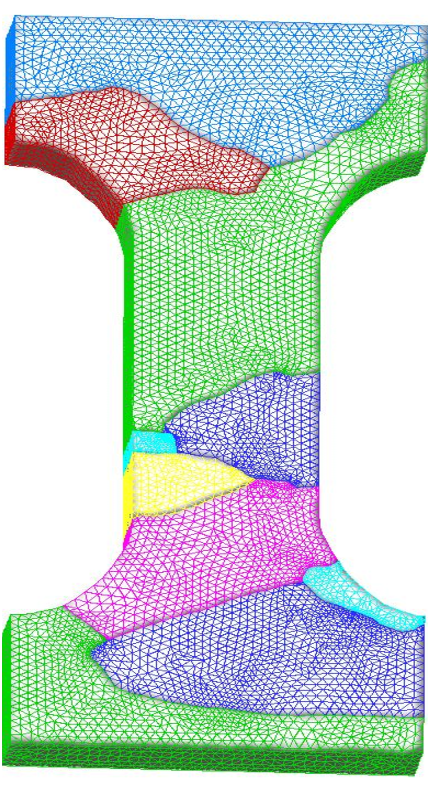
\includegraphics[scale=0.3]{figures/mesh-dogbone.pdf}
  \end{minipage} 
%
\end{frame}

% --------------------------------------
% graph partitioning
\begin{frame}[fragile]
%
  \frametitle{Graph partitioning}
%
  \begin{itemize}
%
  \item 
%
  \end{itemize}
%
\end{frame}

% --------------------------------------
% uniform subdivision
\begin{frame}[fragile]
%
  \frametitle{Uniform subdivision}
%
  \begin{itemize}
%
  \item high fidelity simulations require high resolution
    \begin{itemize}
    \item i.e.~small elements, which implies large element counts
    \item many interesting problems require tens or hundreds of millions of elements before
      they converge
    \item creating input meshes of this size sequentially is impractical
    \end{itemize}
%
  \item one possibility is {\em parallel uniform subdivision}
    \begin{itemize}
    \item the input mesh is partitioned and distributed among processes
    \item each process subdivides its simplices
      \begin{itemize}
      \item edges get split in two, triangles in four, tetrahedra in eight
      \item mesh quality is not affected significantly: only two new classes of simplices are
        introduced, regardless of the number of subdivision levels
      \item the formation of new entities on partition boundaries implies the recalculation of
        the communications maps among processes
      \end{itemize}
    \end{itemize}
%
  \begin{minipage}{.6\linewidth}
    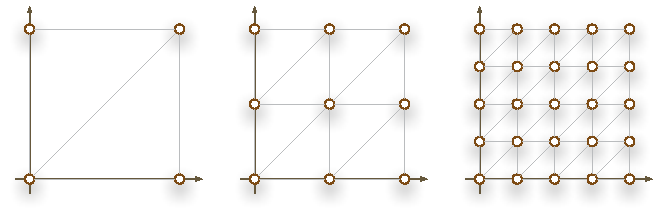
\includegraphics[scale=0.5]{figures/mesh-subdivision.pdf}
  \end{minipage}
    \hfill
  \begin{minipage}{.35\linewidth}
    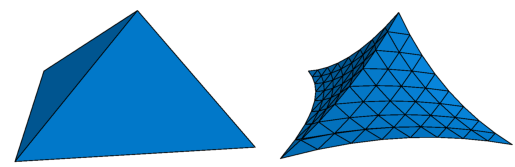
\includegraphics[scale=0.5]{figures/mesh-tetsubdivision.pdf}
  \end{minipage}
%
  \item can be done in linear time
    \begin{itemize}
    \item scales well and can create enormous meshes (billions of elements)
    \end{itemize}
%
  \end{itemize}
%
\end{frame}

% --------------------------------------
% non-uniform subdivision
\begin{frame}[fragile]
%
  \frametitle{Non-uniform subdivision and adaptive remeshing}
%
  \begin{itemize}
%
  \item there are many good non-uniform subdivision algorithms
    \begin{itemize}
    \item e.g.~longest edge subdivision: each tetrahedron that has an edge longer than some
      threshold gets subdivided by splitting that edge in two and connecting the new node to
      the two non-adjacent vertices
    \end{itemize}
%
  \item they tend to be difficult to parallelize because they induce {\em one-sided}
    topological changes on the partition boundaries that must be communicated to the
    neighboring process
    \begin{itemize}
    \item hence they are rarely used in large scale calculations
    \item this is  an {\em architectural} limitation, not an {\em algorithmic} one!
    \item it requires restructuring the solver to support non-trivial communication with its
      neighbors
    \end{itemize}
%
  \item similar considerations apply to adaptive remeshing
    \begin{itemize}
    \item where a process discovers that it requires a higher element density to satisfy some
      correctness criterion
    \item but difficult to implement when the refinement reaches the partition boundary
    \end{itemize}
%
  \end{itemize}
%
\end{frame}

% --------------------------------------
% fracture and fragmentation
\begin{frame}[fragile]
%
  \frametitle{Fracture and fragmentation}
%
  \begin{itemize}
%
  \item when the material is under sufficient tension, modeling the physics correctly
    requires topological changes to the mesh
    \begin{itemize}
    \item the material {\em fractures} when it is energetically favorable for an opening to
      form between two elements that are being pulled apart
    \end{itemize}
%
  \item modeling this typically involves {\em cohesive elements}
    \begin{itemize}
    \item prismatic elements that are inserted in the place of what used to be the common face
      of two tetrahedra and absorb excess energy
    \end{itemize}
%
  \item when some threshold is exceeded, the cohesive element fractures and becomes free
    surface
%
  \item cohesive element insertion involves node, edge and face splitting
  \item difficulties arise as cracks run up to process boundaries and must be propagated across
  \item eventually, fragments form as cracks disconnect portions of the mesh
%
  \end{itemize}
%
  \begin{figure}
    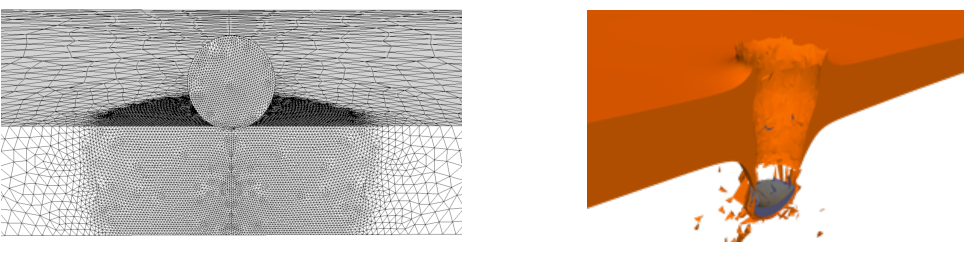
\includegraphics[scale=0.5]{figures/mesh-penetration.pdf}
  \end{figure}
%
\end{frame}

% --------------------------------------
% contact detection
\begin{frame}[fragile]
%
  \frametitle{Contact detection}
%
  \begin{itemize}
%
  \item modeling impact requires detecting when bodies come into contact and computing
    appropriate forces
    \begin{itemize}
    \item both are difficult problems, especially for non-smooth, distributed meshes
    \item the computations involve only elements on the free boundary
    \end{itemize}
%
  \item the element updates and contact search have very different communication patterns
    \begin{itemize}
    \item contact is {\em global}, since any two surface triangles can collide
    \item and it is expensive, since it involves geometrical queries
    \item it is best solved as an auxiliary parallel problem with its own partitioning
      \begin{itemize}
      \item boundary partitioned using geometric criteria, such as axis-aligned cutting planes
      \item requires frequent re-balancing as mesh geometry and topology change
      \end{itemize}
    \end{itemize}
%
  \item in {\em surface driven} contact detection
    \begin{itemize}
    \item the boundary is partitioned and the centers of all the faces are inserted in some
      kind of spatial data structure
      \begin{itemize}
      \item so that coarse calculations about contact candidates can be made efficiently
      \item typically bucket or sparse-bucket arrays that support {\em orthogonal range
          queries} (ORQ)
      \end{itemize}
    \item candidates can be checked pairwise for actual contact using ray-triangle and
      edge-triangle intersection algorithms
    \end{itemize}
%
  \end{itemize}
%
\end{frame}

% --------------------------------------
% volume-based contact detection
\begin{frame}[fragile]
%
  \frametitle{Volume based contact detection}
%
  \begin{itemize}
%
  \item volume based approaches replace the elements on the boundary with equivalent spheres
  \item a variety of geometrical criteria can be used: 
    \begin{itemize}
      \item equivalent volume
      \item diameter determined by the longest edge
    \end{itemize}
% 
  \item contact detection can take place very efficiently using ORQ algorithms
  \item simple spring models resolve the contact forces
    \begin{itemize}
    \item based on simple potentials that take into account the sphere inter-penetration
    \end{itemize}
%
  \end{itemize}
%
  \begin{figure}
    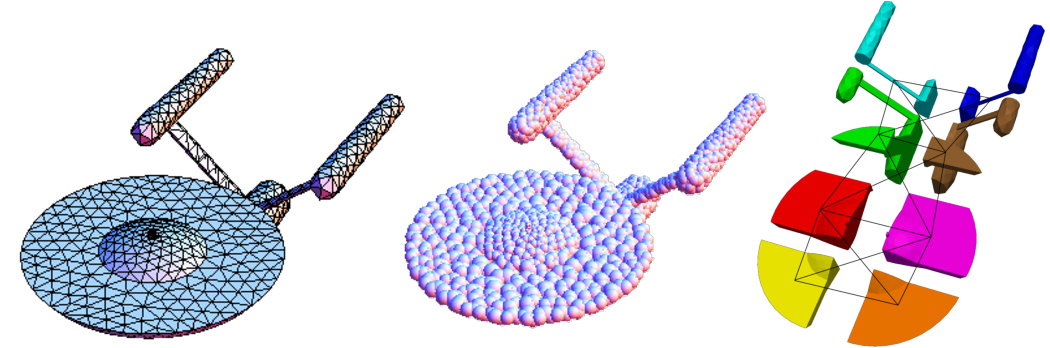
\includegraphics[scale=0.5]{figures/mesh-volumecontact.pdf}
  \end{figure}
%
\end{frame}

% --------------------------------------
% element erosion
\begin{frame}[fragile]
%
  \frametitle{Element erosion}
%
  \begin{itemize}
%
  \item 
%
  \end{itemize}
%
\end{frame}

% --------------------------------------
% mesh optimization
\begin{frame}[fragile]
%
  \frametitle{Mesh optimization}
%
  \begin{itemize}
%
  \item 
%
  \end{itemize}
%
\end{frame}

% --------------------------------------
% level sets
\begin{frame}[fragile]
%
  \frametitle{Implicit representations of surfaces}
%
  \begin{itemize}
%
  \item 
%
  \end{itemize}
%
\end{frame}

% --------------------------------------
% open problems
\begin{frame}[fragile]
%
  \frametitle{Summary of open problems}
%
  \begin{itemize}
%
  \item many interesting physics problems require making topological changes to the simplicial
    meshes, and propagating them across process boundaries
    \begin{itemize}
    \item good sequential algorithms exist, but they are difficult to parallelize
    \item na\"ive parallelization is almost always prohibitively expensive
      \begin{itemize}
      \item because maintaining coherence and consistency of the global information requires a
        lot of communication
      \end{itemize}
    \end{itemize}
%
  \item changing the solver architecture may be key to efficient parallel implementations
    \begin{itemize}
      \item evolving mesh topology requires complicated interactions among processes
      \item {\em event based} solutions enable such interactions
      \item and improve simulation control by external agents
        \begin{itemize}
          \item better monitoring through probes and sensors
          \item {\em instrumentation} for virtual experiments
        \end{itemize}
    \end{itemize}
%
  \end{itemize}
%
\end{frame}

% end of file 

% -*- LaTeX -*-
% -*- coding: utf-8 -*-
%
% ~~~~~~~~~~~~~~~~~~~~~~~~~~~~~~~~~~~~~~~~~~~~~~~~~~~~~~~~~~~~~~~~~~~~~~~~~~~~~~
%
%                             michael a.g. aïvázis
%                      california institute of technology
%                      (c) 1998-2010  all rights reserved
%
% ~~~~~~~~~~~~~~~~~~~~~~~~~~~~~~~~~~~~~~~~~~~~~~~~~~~~~~~~~~~~~~~~~~~~~~~~~~~~~~
%

\lecture{Geometrical}{20100301}

% --------------------------------------
% contact detection
\begin{frame}[fragile]
%
  \frametitle{A more careful look at contact detection}
%
  \begin{itemize}
%
  \item consider a collection of tetrahedral meshes that model bodies in relative motion with
    triangular meshes as boundaries
%
  \item during the simulation, the bodies may come in contact
    \begin{itemize}
    \item with each other or themselves
    \item {\em contact events} consist of intersections among nodes, edges or faces
    \item unless the mechanics is informed of the contact events, the objects will
      inter-penetrate
    \item contact {\em detection} involves isolating the pairs of topological entities from
      each boundary that have intersected, whereas contact {\em resolution} refers to the
      calculation of appropriate restoring forces on the bodies
    \end{itemize}
%
  \item the typical simulation update step proceeds along the following lines
    \begin{enumerate}
    \item define the contact surfaces at time $t$
    \item predict the location of the nodes at a later time $t+\Delta t$ by integrating the
      equations of motion
    \item search for potential contact events among nodes, edges and faces to identify the
      entities that come in contact \label{item:contact-search}
    \item correct the future location of the nodes by applying forces that tend to remove the
      overlap
    \end{enumerate}
%
  \end{itemize}
%
\end{frame}

% --------------------------------------
% contact search
\begin{frame}[fragile]
%
  \frametitle{Contact search}
%
  \begin{itemize}
%
  \item the contact event identification in Step~\ref{item:contact-search} above has the
    potential to dominate the calculation
    \begin{itemize}
    \item given a candidate pair, the intersection logic involves very expensive geometrical
      calculations
    \item na\"ive algorithms are \order{n^{2}} in the number of topological entities on the
      boundary, prohibitively expensive even for moderate size calculations
    \end{itemize}
%
  \item hence, a more sensible strategy is to break up the contact search into two separate steps
    \begin{itemize}
    \item use a specialized data structure that encodes the location of mesh nodes and build a
      relatively fast algorithm to narrow down the candidates to a small number
    \item perform the detailed calculations on the reduced set
    \end{itemize}
%
  \item typically, the fast searches are implemented using {\em orthogonal range queries} that
    identify points whose co\"ordinates fall within a given box
    \begin{itemize}
    \item build a bounding box that contains the initial and final position of a given surface
      element, perhaps in some reduced form 
    \item form the {\em capture box} by enlarging the bounding box to account for the motion of
      the nodes
    \item query the data structure for nodes that fall within the capture box
    \end{itemize}
%
  \end{itemize}
%
\end{frame}

% --------------------------------------
% overview of contact
\begin{frame}[fragile]
%
  \frametitle{Orthogonal range queries}
%
  \begin{minipage}{.70\linewidth}
%
  \begin{itemize}
%
  \item an orthogonal range query is a generalization of the interval test to higher dimensions
    \begin{itemize}
    \item given a number $p$ and an interval $[a,b)$, return \keyword{true} if the number falls
    within the interval, otherwise return \keyword{false}
    \item extend by performing a test for each co\"ordinate: does the point $p$ fall within a
      given box?
    \end{itemize}
%
  \item there is a variety of data structures that are {\em a priori} well suited to this
    problem
    \begin{itemize}
    \item however, the problem context establishes some crucial constraints
    \end{itemize}
%
  \end{itemize}
%
  \end{minipage}
%
  \hfill
  \begin{minipage}{.27\linewidth}
    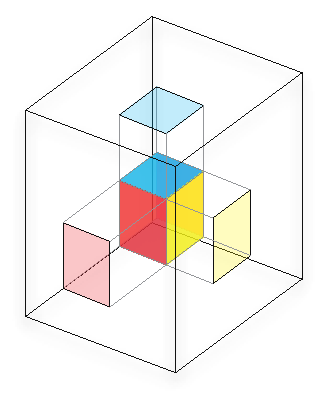
\includegraphics[scale=0.7]{figures/orq.pdf}
  \end{minipage} 
%
  \begin{itemize}
%
  \item we will classify algorithms according to the following metrics
    \begin{itemize}
    \item $b(N)$: the time it takes to initially populate the data structure with $N$ points
    \item $r(N)$: the complexity of rebuilding or update the data structure
    \item $s(N)$: the amount of storage required
    \item $q(N,n)$ and $\bar{q}(N,n)$: the (average) time required to perform a query if
      there are $n$ points in the given range
    \end{itemize}
%
  \item also, we'll start out in one dimension and generalize
%
  \end{itemize}
%
\end{frame}

% --------------------------------------
% simple algorithms
\begin{frame}[fragile]
%
  \frametitle{Sequential scan}
%
  \begin{itemize}
%
  \item the simplest approach is to look at each record and determine whether it falls in the
    range
    \begin{itemize}
    \item this algorithm is trivial to implement and requires no extra storage
    \item the performance is acceptable for sufficiently small $N$, or if most of the records
      fall in the query interval
      \begin{equation*}
        \begin{array}{rclcrcl}
          b_{{\tt SCAN}} & = & \order{N} &, &
          r_{{\tt SCAN}} & = & 0  \\
          s_{{\tt SCAN}} & = & \order{N} &, &
          q_{{\tt SCAN}} & = & \order{N}
        \end{array}
      \end{equation*}
    \end{itemize}
%
  \end{itemize}
%
  \begin{center}
    \begin{minipage}{.85\linewidth}
      \begin{algorithm}[H]
        \label{alg:rq-scan}
%
        \dontprintsemicolon
        % \nocaptionofalgo
        \setalcaphskip{0ex}
%
        \caption{\rqscan(points, interval)}
%
        $candidates \leftarrow \emptyset$ \;
        \For{$point$ \In $points$}{
          \If {$point \in interval$} {
            $candidates.insert(point)$
          }
        }
        \Return{$candidates$}
%
      \end{algorithm}
    \end{minipage}
  \end{center}
%
\end{frame}

% --------------------------------------
% simple algorithms
\begin{frame}[fragile]
%
  \frametitle{Binary search}
%
  \begin{itemize}
%
  \item if the records are sorted, a binary search can locate any record with cost $\order{\log
      N}$, so in order to find all $p \in [a,b)$
    \begin{itemize}
    \item find the first point that satisfies $p >= a$
    \item and collect points in sequence while $p < b$
    \item simple analysis yields
      \begin{equation*}
        \begin{array}{rclcrcl}
          b_{{\tt BS}} & = & \order{N \log N} &, &
          r_{{\tt BS}} & = & \order{N} \\
          s_{{\tt BS}} & = & \order{N} &, &
          q_{{\tt BS}} & = & \order{\log N + n}
        \end{array}
      \end{equation*}
      since the records must be sorted initially, while rebuilding the data structure can be
      done in linear time since it is almost sorted
    \end{itemize}
% 
  \end{itemize}
%
  \begin{center}
    \begin{minipage}{.85\linewidth}
      \begin{algorithm}[H]
        \label{alg:rq-bs}
%
        \dontprintsemicolon
        % \nocaptionofalgo
        \setalcaphskip{0ex}
%
        \caption{\rqbs(points, interval=(a,b))}
        \vspace{.5em}
%
        $candidates \leftarrow \emptyset$ \;
        $iterator \leftarrow \bslb(points, a)$ \;
        \While{$\star iterator \leq b$}{
          \If {$point \in interval$} {
            $candidates.insert(point)$
          }
        }
        \Return{$candidates$}
%
      \end{algorithm}
    \end{minipage}
  \end{center}
%
\end{frame}

% --------------------------------------
% using trees
\begin{frame}[fragile]
%
  \frametitle{Tricks with trees}
%
  \begin{itemize}
%
  \item alternatively, we can store the points at the leaves of a binary tree data structure
    \begin{itemize}
    \item each internal tree node acts has a {\em discriminator} that splits the data set into
      two subsets
    \item numbers less than the discriminator go to the left branch, the rest to the right
    \item once the population drops below some threshold, create a leaf node to hold the points
    \end{itemize}
%
%
  \item two sensible choices for the discriminator are
    \begin{itemize}
    \item the midpoint of the interval: yields a recursive subdivision of the interval
      \begin{itemize}
      \item also known as interval trees or {\em orthotrees}
      \item quadtrees in two dimensions, octrees in three
      \end{itemize}
    \item the median of the data set: partitions the data in subsets of equal size
      \begin{itemize}
      \item $kd$ trees
      \end{itemize}
    \end{itemize}
%
  \end{itemize}
%
\end{frame}

% --------------------------------------
% creating a binary tree
\begin{frame}[fragile]
%
  \frametitle{Creating a binary tree}
%
  \begin{center}
    \begin{minipage}{.85\linewidth}
      \begin{algorithm}[H]
        \label{alg:binary-tree}
%
        \dontprintsemicolon
        % \nocaptionofalgo
        \setalcaphskip{0ex}
%
        \caption{\treemake(points)}
        \vspace{.5em}
%
        \If{$length[points] < tree.leafSize$}{
          $leaf \leftarrow tree.newLeaf()$ \;
          $leaf.insert(points)$ \;
          \Return{$leaf$}
        }\Else{
          $branch \leftarrow tree.newBranch()$ \;
          select branch $discriminator$ \;
          $left \leftarrow \left\{ x \in points : x < discriminator \right\}$ \;
          $branch.left \leftarrow tree.make(left)$ \;
          $right \leftarrow \left\{ x \in points : x >= discriminator \right\}$ \;
          $branch.right \leftarrow tree.make(right)$ \;
          \Return{branch}
        }
%
      \end{algorithm}
    \end{minipage}
  \end{center}
%
\end{frame}

% --------------------------------------
% range query in a binary tree
\begin{frame}[fragile]
%
  \frametitle{Querying a binary tree}
%
  \begin{center}
    \begin{minipage}{.85\linewidth}
      \begin{algorithm}[H]
        \label{alg:rq-tree}
%
        \dontprintsemicolon
        % \nocaptionofalgo
        \setalcaphskip{0ex}
%
        \caption{\rqtree(tree, interval=(a,b))}
        \vspace{.5em}
%
        \If{$tree$ \Is $leaf$}{
          \Return{$\rqscan(tree.points, interval)$}
        }\Else{
          $candidates \leftarrow \emptyset$ \;
          \If {$tree.discriminator \geq a$} {
            $candidates \leftarrow candidates + \rqtree(tree.left, interval)$ \;
          }
          \If {$tree.discriminator < b$} {
            $candidates \leftarrow candidates + \rqtree(tree.right, interval)$ \;
          }
          \Return{$candidates$}
        }
%
      \end{algorithm}
    \end{minipage}
  \end{center}
%
\end{frame}

% --------------------------------------
% binary tree performance
\begin{frame}[fragile]
%
  \frametitle{Performance of binary trees}
%
  \begin{itemize}
%
  \item for midpoint splitting, the depth $D$ of the tree depends on the point distribution
    \begin{equation*}
      \begin{array}{lll}
        b_{{\tt ORTHO}} = \order{(D+1)N} &
        r_{{\tt ORTHO}} = \order{(D+1)N}  \\
        s_{{\tt ORTHO}} = \order{(D+1)N} &
        q_{{\tt ORTHO}} = \order{N} &
        \bar{q}_{{\tt ORTHO}} = \order{D+n}
      \end{array}
    \end{equation*}
%
  \item for median splitting the depth of the tree depends only on the number of records
    \begin{equation*}
      \begin{array}{ll}
        b_{{\tt KD}} = \order{N \log N} &
        r_{{\tt KD}} = \order{N}  \\
        s_{{\tt KD}} = \order{N} &
        q_{{\tt KD}} = \order{n + \log N}
      \end{array}
    \end{equation*}
%
  \end{itemize}
%
\end{frame}

% --------------------------------------
% binning in buckets
\begin{frame}[fragile]
%
  \frametitle{Binning}
%
  \begin{itemize}
%
  \item another strategy is to partition the interval $[a,b)$ into $M$ cells of width
    \[
    \delta \bydef x_{m+1} - x_{m} = \frac{b-a}{M}
    \]
    \begin{itemize}
    \item the \th{m} cell $C_{m}$ holds points in the interval $[x_{m}, x_{m+1})$
    \item the point container then becomes an array of $M$ point containers
    \item and the array index for a point $p$ is obtained through
      \[
      i = \lfloor \frac{p-a}{\delta} \rfloor
      \]
    \end{itemize}
%
  \item the process of putting the points in the container is known as a {\em cell sort}
%
  \item they are optimal when properly tuned
      \begin{equation*}
        \begin{array}{lll}
          b_{{\tt CELL}} = \order{N + M} &
          r_{{\tt CELL}} = \order{N + M} \\
          s_{{\tt CELL}} = \order{N + M} &
          q_{{\tt CELL}} = \order{J + n} &
          \bar{q}_{{\tt CELL}} = \order{n}
        \end{array}
      \end{equation*}
      where $J$ is the number of cells that overlap the query interval
%
  \end{itemize}
%
\end{frame}

% --------------------------------------
% range query in a cell array tree
\begin{frame}[fragile]
%
  \frametitle{Querying a cell array}
%
  \begin{center}
    \begin{minipage}{.85\linewidth}
      \begin{algorithm}[H]
        \label{alg:rq-cell}
%
        \dontprintsemicolon
        % \nocaptionofalgo
        \setalcaphskip{0ex}
%
        \caption{\rqcell(cells, interval=(a,b))}
        \vspace{.5em}
%
        $candidates \leftarrow \emptyset$ \;
        $i \leftarrow index(cells, a)$ \;
        $j \leftarrow index(cells, b)$ \;
        \For{$point$ \In $cells[i]$}{
          \If{$point \geq a$}{
            $candidates.insert(point)$ \;
          }
        }
        \For{$k$ \In $[i+1 .. j-1]$}{
          \If{$point$ \In $cells[k]$}{
            $candidates.insert(point)$ \;
          }
        }
        \For{$point$ \In $cells[j]$}{
          \If{$point < b$}{
            $candidates.insert(point)$ \;
          }
        }
        \Return{$candidates$}
%
      \end{algorithm}
    \end{minipage}
  \end{center}
%
\end{frame}

% --------------------------------------
% higher dimensions
\begin{frame}[fragile]
%
  \frametitle{Generalizing to higher dimensions}
%
  \begin{itemize}
%
  \item the sequential scan algorithm has trivial generalizations
    \begin{itemize}
    \item its performance is only acceptable for very small numbers of points
    \item frequently used by the other algorithms to manage small size point sets
    \end{itemize}
%
  \item binary search generalizes to the {\em projection} method in $d$ dimensions
    \begin{itemize}
    \item sort the points according to their \th{k} co\"ordinate and build a reference set for
      this ordering
    \item for example, one can number the points, sort them according to each co\"ordinate, and
      build arrays of the point indices, or arrays of pointers to the actual data
    \item a range query along any dimension yields all the points that lie within a slice of
      the domain
    \item to perform an orthogonal range query
      \begin{itemize}
      \item perform a range query along each dimension using binary searches
      \item identify the co\"ordinate slice with the fewest records
      \item perform a sequential scan
      \end{itemize}
    \end{itemize}
%
  \end{itemize}
%
\end{frame}

% --------------------------------------
% kd tree
% s
\begin{frame}[fragile]
%
  \frametitle{$kd$ trees}
%
  \begin{itemize}
%
  \item in $d$ dimensions, there is a median point for each co\"ordinate
    \begin{itemize}
    \item split the tree using the co\"ordinate with the largest spread
    \item repeat this process at each level of the tree until the number of points to insert
      into the tree drops below some threshold
    \item every internal node of the tree has to record at least
      \begin{itemize}
      \item the direction that was chosen for the split
      \item the value of the discriminant
      \item references to the left and right branches of the node
      \end{itemize}
    \item leaf nodes are just point containers
    \end{itemize}
%
  \item the orthogonal range query is defined recursively
    \begin{itemize}
    \item at each internal node, check whether the left and right subdomains intersect the
      query interval by examining the discriminator
    \item recurse into the branches that intersect the range
    \item leaf nodes are examined using a sequential search
    \end{itemize}
%
  \end{itemize}
%
  \begin{figure}
    \begin{minipage}{0.75\linewidth}
    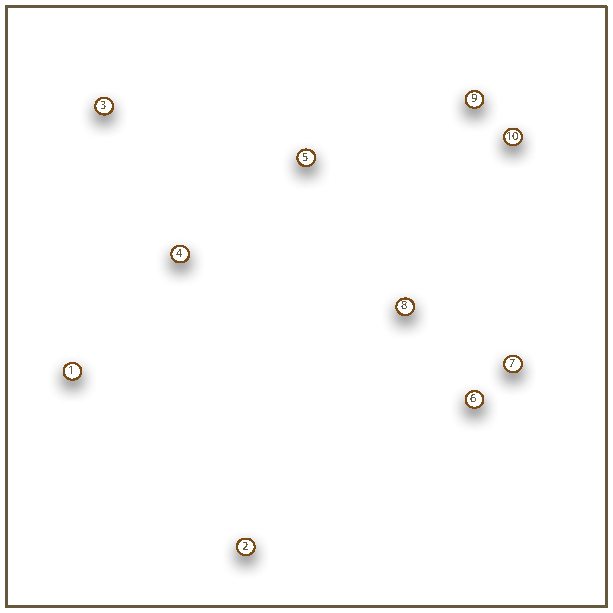
\includegraphics[scale=0.2]{figures/spatial-points.pdf}
    \hfill
    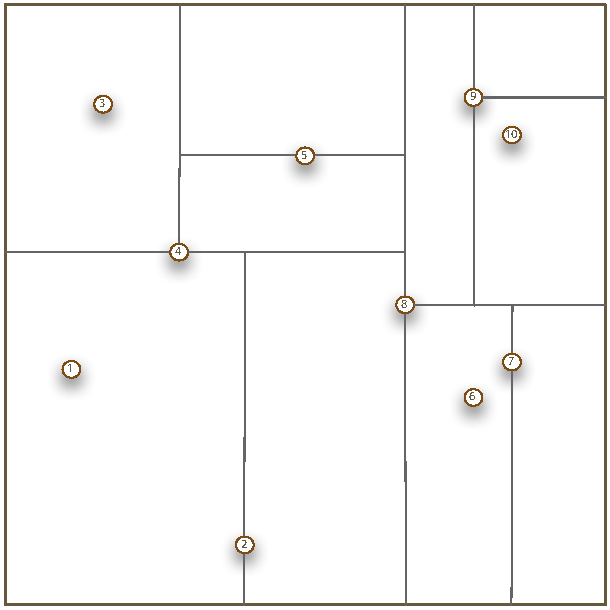
\includegraphics[scale=0.2]{figures/spatial-kd-split.pdf}
    \hfill
    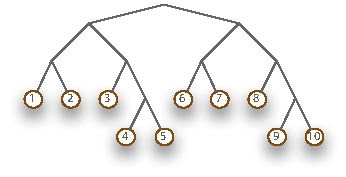
\includegraphics[scale=0.6]{figures/spatial-kd-tree.pdf}
  \end{minipage}
  \end{figure}
%
\end{frame}

% --------------------------------------
% orthotrees
\begin{frame}[fragile]
%
  \frametitle{Orthotrees}
%
  \begin{itemize}
%
  \item orthotrees are the generalization of interval trees in $d$ dimensions
    \begin{itemize}
    \item commonly known as {\em quadtrees} in two dimensions, and {\em octrees} in three
    \item recursively split the $d$-dimensional domain into $2^{d}$ equal size hyperboxes
    \item each internal node has $2^{d}$ branches
    \item some of the branches lead to leaf nodes that contain the actual data
    \end{itemize}
%
  \item the depth of the tree depends on the actual distribution of points in the input set
    \begin{itemize}
    \item points that are very close to each other could lead to some very deep trees
    \end{itemize}
%
  \item orthogonal range queries are implemented similarly to $kd$ trees
%
  \end{itemize}
%
  \begin{figure}
    \begin{minipage}{0.75\linewidth}
    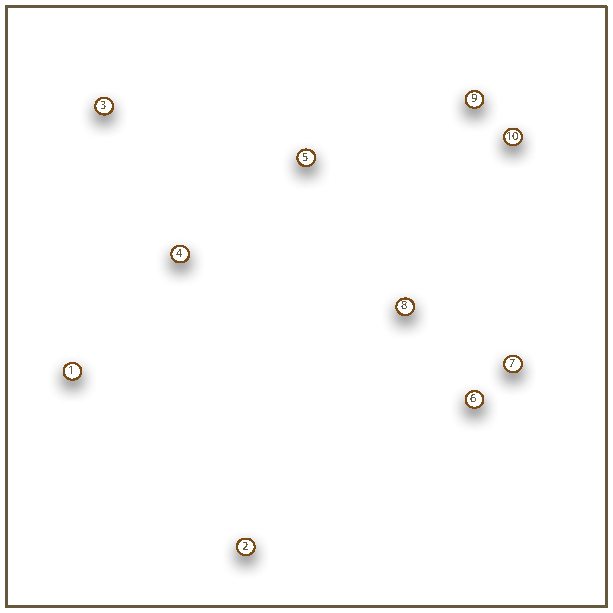
\includegraphics[scale=0.2]{figures/spatial-points.pdf}
    \hfill
    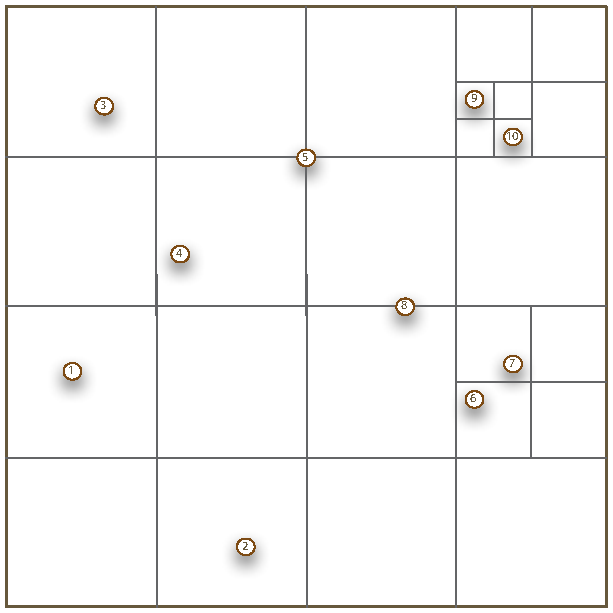
\includegraphics[scale=0.2]{figures/spatial-ortho-split.pdf}
    \hfill
    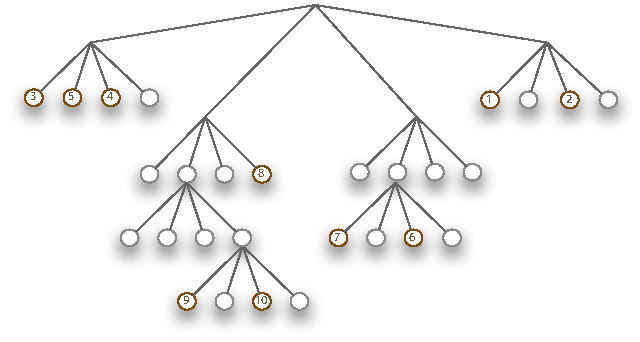
\includegraphics[scale=0.3]{figures/spatial-ortho-tree.pdf}
  \end{minipage}
  \end{figure}
%
\end{frame}

% --------------------------------------
% cells
\begin{frame}[fragile]
%
  \frametitle{Binning in higher dimensions}
%
  \begin{itemize}
%
  \item cell sort extends naturally to $d$ dimensions
    \begin{itemize}
    \item form a regular grid of spacing $\delta_{i}$ along the \th{i} dimension
    \item convert the point coordinates into cell indices along each dimension using the same
      formula as in one dimension
    \end{itemize}
%
    \item the orthogonal range query consists of accessing cells that
      \begin{itemize}
      \item entirely interior to the query box
      \item partially overlap the boundary of the query box
      \item the former are unconditionally included in the candidate list, while point in the
        latter must be checked individually
      \end{itemize}
%
    \item tuning is crucial to the performance of this method
      \begin{itemize}
      \item cells that are too large can lead to many false positives
      \item cells that are too small have higher access times
      \item it is best to know the size of the query boxes so that the cell spacing can be
        optimized
      \end{itemize}
%
    \item can be easily combined with any of the other methods to speed up access to the points
      in each cell
      \begin{itemize}
      \item most combinations do not offer significant advantages
      \item but using binary searches is an exception
      \end{itemize}
%
  \end{itemize}
%
\end{frame}

% --------------------------------------
% parallelization
\begin{frame}[fragile]
%
  \frametitle{Parallelization}
%
  \begin{itemize}
%
  \item minimization of the communication cost
    \begin{itemize}
    \item best to avoid communication altogether if possible
    \item any type of globally distributed data structure would eventually dominate the
      calculation
    \item so would global data exchanges to maintain locally consistent information
    \end{itemize}
  \item load balancing
    \begin{itemize}
    \item the parallel characteristics of contact are different from the solver update
    \item it is probably unavoidable that a few processors will be responsible for detecting and
      resolving the bulk of contact
    \end{itemize}
%
  \item utilize point-to-point communications as much as possible
    \begin{itemize}
    \item build/exchange bounding boxes for the geometry kept by each processor
    \item use it to build point-to-point communication maps
    \item exchange boundary elements so contact resolution can happen locally
    \item exchange the resulting forces
    \end{itemize}
%
  \item a research problem
    \begin{itemize}
    \item we know that processing multiple queries has better parallel characteristics than a
      single one
    \item we need a self-balancing, dynamically repartitioning data structure
    \end{itemize}
%
  \end{itemize}
%
\end{frame}


% end of file 

% -*- LaTeX -*-
% -*- coding: utf-8 -*-
%
% ~~~~~~~~~~~~~~~~~~~~~~~~~~~~~~~~~~~~~~~~~~~~~~~~~~~~~~~~~~~~~~~~~~~~~~~~~~~~~~
%
%                             michael a.g. aïvázis
%                      california institute of technology
%                      (c) 1998-2010  all rights reserved
%
% ~~~~~~~~~~~~~~~~~~~~~~~~~~~~~~~~~~~~~~~~~~~~~~~~~~~~~~~~~~~~~~~~~~~~~~~~~~~~~~
%

\lecture{Matrices}{20100303}

% --------------------------------------
% contact detection
\begin{frame}[fragile]
%
  \frametitle{Dense matrix problems}
%
  \begin{itemize}
%
  \item we'll take a look at
    \begin{itemize}
    \item inner and outer products of two vector
    \item matrix-vector and matrix-matrix multiplication
    \item $LU$ factorization and Cholesky decomposition
    \item QR factorization
    \item computing eigenvalues and eigenvectors
    \item fast Fourier transforms
    \end{itemize}
%
  \item when solving a problem of size $n$ on $p$ processors, we will assume
    \begin{itemize}
    \item that $p$, and occasionally $\sqrt{p}$ divides $n$
    \item that $p$ is a perfect square, when forming two-dimensional process grids
    \item matrices are $n\times n$ -- square, not rectangular
    \item we are memory constrained and data replication must be minimized
    \end{itemize}
%
    \item these problems have been studied extensively and form the core of scientific
      computing on parallel machines
      \begin{itemize}
      \item excellent implementations available 
      \item interest has been revived due to the expected disruption by multi-core
        architectures
      \end{itemize}
%
  \end{itemize}
%
\end{frame}

% --------------------------------------
% vector inner product
\begin{frame}[fragile]
%
  \frametitle{Vector inner product}
%
  \begin{itemize}
%
  \item the inner product of two $n$-vectors $x$, $y$ is given by
    \begin{equation}
    x^{T}y = \sum_{i=1}^{n} x_{i}y_{i}
    \end{equation}
    which requires $n$ multiplications and $n-1$ additions
%
  \item parallelization strategy:
    \begin{itemize}
    \item $n$ fine grain tasks, numbered $i = 1, \ldots, n$, that store $x_{i}$ and $y_{i}$,
      and compute $x_{i} y_{i}$
    \item communication is a sum reduction over $n$ fine grain tasks
    \item coarsening is achieved by coalescing $n/p$ tasks together, assuming that each process
      can accommodate the data storage requirements
    \item and mapping each coarse grain task to a process
    \end{itemize}
%
  \end{itemize}
%
\end{frame}

% --------------------------------------
% vector outer product
\begin{frame}[fragile]
%
  \frametitle{Vector outer product}
%
  \begin{itemize}
%
  \item the outer product of two $n$-vectors $x$ and $y$ is the $n \times n$ matrix $A$ given
    by
    \begin{equation}
      A_{ij} = x_{i} y_{j}
    \end{equation}
    which requires $n^{2}$ multiplications
%
  \item parallelization strategies are determined by the storage requirements
    \begin{itemize}
    \item build a two-dimensional grid of $n^{2}$ fine grain tasks numbered $(i,j)$, with $i,j
      = 1, \ldots, n$; each one computes $x_{i}y_{j}$
    \item assuming no data replication is allowed
      \begin{itemize}
      \item let task $(i,1)$ store $x_{i}$ and task $(1,i)$ store $y_{i}$
      \item or, let task $(i,i)$ store both $x_{i}$ and $y_{i}$
      \end{itemize}
    \item either way, the task that owns each element must broadcast it to the other tasks:
      $x_{i}$ along the \th{i} task row, $y_{j}$ along the \th{j} task column
    \item coarsening to $p$ tasks can be accomplished by
      \begin{itemize}
      \item combining $n/p$ rows or columns
      \item forming $(n/\sqrt{p}) \times (n/\sqrt{p})$ grid of fine grain tasks
      \end{itemize}
    \item and each coarse grain task can be assigned to a process
    \end{itemize}
%
  \item either way, na\"ive broadcasting of the components of $x$ and $y$ would require as much
    total memory as replication
    \begin{itemize}
    \item storage can be reduced by circulating portions of $x$ and $y$ through the tasks, with
      each task using the available portion and passing it on
    \end{itemize}
%
  \end{itemize}
%
\end{frame}

% --------------------------------------
% matrix vector product
\begin{frame}[fragile]
%
  \frametitle{The product of a matrix with a vector}
%
  \begin{itemize}
%
  \item given an $n \times n$ matrix $A$ and an $n$-vector $x$, the matrix vector product
    yields an $n$-vector $y$ whose components are given by
    \begin{equation}
      y_{i} = \sum_{j=1}^{n} A_{ij} x_{j}
    \end{equation}
    requiring a total of $n^{2}$ multiply-add operations
%
  \item once again, the parallelization strategy is determined by how the data is distributed
    among fine grain tasks
    \begin{itemize}
    \item build a two-dimensional grid of $n^{2}$ fine grain tasks numbered $(i,j)$, with $i,j
      = 1, \ldots, n$; each one computes $A_{ij}x_{j}$
    \item task $(i,j)$ has $A_{i,j}$, but if no data replication is allowed
      \begin{itemize}
      \item let task $(i,1)$ store $x_{i}$ and task $(1,i)$ store $y_{i}$
      \item or, let task $(i,i)$ store both $x_{i}$ and $y_{i}$
      \end{itemize}
    \item the task that owns $x_{j}$ must broadcast it along the \th{j} task row, and $y_{i}$
      is formed by sum reduction along the \th{i} task column
    \item coarsening into $p$ tasks can be accomplished by combining $n/p$ rows/columns, or by
      forming $(n/\sqrt{p}) \times (n/\sqrt{p})$ blocks
    \item and each coarse grain task can be assigned to a process
    \end{itemize}
%
  \end{itemize}
%
\end{frame}

% --------------------------------------
% coarsening matrix vector product
\begin{frame}[fragile]
%
  \frametitle{Coarsening along rows or columns}
%
  \begin{itemize}
%
  \item for one-dimensional coarsening into $n/p$ task rows
    \begin{itemize}
    \item if $x$ is stored in one task, it must be broadcast to all others
    \item if $x$ is distributed among tasks, with $n/p$ components per task, then multiple
      broadcasts are required
    \item each task computes the inner product of its $n/p$ rows of $A$ with the entire $x$ to
      produce $n/p$ components of $y$
    \end{itemize}
%
  \item for one-dimensional coarsening into $n/p$ task columns
    \begin{itemize}
    \item $n/p$ components of $x$ are distributed among the tasks
    \item each task computes the linear combination of its $n/p$ columns with coefficients
      from its copy of $x$
    \item since the right parts of $x$ are already available, no communication is required
    \item $y$ is generated by a sum reduction across tasks
    \end{itemize}
%
  \item these two are {\em duals} of each other
    \begin{itemize}
    \item row coarsening begins with broadcast, followed by communication-free inner products
    \item column coarsening begins with communication-free linear combinations, follows by a
      reduction
    \end{itemize}
%
  \end{itemize}
%
\end{frame}

% --------------------------------------
% 2d coarsening
\begin{frame}[fragile]
%
  \frametitle{Two dimensional coarsening}
%
  \begin{itemize}
%
  \item for two dimensional coarsening, we form $(n/\sqrt{p}) \times (n/\sqrt{p})$ blocks of
    fine grain task
    \begin{itemize}
    \item each one holding a $(n/\sqrt{p}) \times (n/\sqrt{p})$ block of $A$
    \item with components of $x$ distributed either across one task row, or along the diagonal,
      $n/p$ components per task
    \end{itemize}
%
  \item the algorithm combines the features of row/column coarsening
    \begin{itemize}
    \item components of $x$ are broadcast along task columns
    \item each task performs $n^{2}/p$ multiplications locally and sums $n/\sqrt{p}$ sets of
      products
      \item sum reductions along task rows produce the components of $y$ by combining the
        component products
    \end{itemize}
%
  \end{itemize}
%
\end{frame}

% --------------------------------------
% matrix-matrix multiply
\begin{frame}[fragile]
%
  \frametitle{Matrix multiplication}
%
  \begin{itemize}
%
  \item the product of two $n \times n$ matrices $A$ and $B$ is an $n \times n$ matrix $C$
    given by
    \begin{equation}
      C_{ij} = \sum_{k=1}^{n} A_{ik} B_{kj}
    \end{equation}
    where each one of $n^{2}$ entries requires $n$ multiply-adds for a total of $n^{3}$
    operations
%
  \item matrix multiplication can be viewed as
    \begin{itemize}
    \item $n^{2}$ inner products
    \item the sum of $n$ outer products
    \item $n$ matrix vector products
    \end{itemize}
%
  \item each one produces a parallel algorithm for matrix multiplication
%
  \item but we'll explore a direct solution instead
%
  \end{itemize}
%
\end{frame}

% --------------------------------------
% matrix-matrix multiply: partitioning and communication
\begin{frame}[fragile]
%
  \frametitle{Partitioning and communication patterns}
%
  \begin{itemize}
%
  \item we build a three dimensional array of $n^{3}$ fine grain tasks
    \begin{itemize}
    \item with $i,j,k = 1,\ldots,n$, let task $(i,j,k)$ be responsible for computing the
      product $A_{ij}B_{jk}$
    \item assuming no data replication, we have to distribute the data for $A$ and $B$ among
      $2n^{2}$ tasks
    \item suppose that task $(i,j,j)$ holds $A_{i,j}$ and task $(i,j,i)$ holds $B_{i,j}$
    \item we will refer to tasks along $i$ and $j$ as task rows and columns
    \item and tasks along $k$ as {\em layers}
    \end{itemize}
%
  \item the communication requirements among tasks are satisfied if we
    \begin{itemize}
    \item broadcast the entries of the \th{k} column of $A$ from task $(i,j,j)$ to each task
      row in the \th{k} layer
    \item broadcast the entries of the \th{k} row of $B$ from task $(i,j,i)$ to each task column of
      the \th{k} layer
    \item form the result $C_{ij}$ by the sum reduction of the values held by all the
      tasks layers $k$
    \end{itemize}
%
  \end{itemize}
%
\end{frame}

% --------------------------------------
% coarsening
\begin{frame}[fragile]
%
  \frametitle{Coarsening}
%
  \begin{itemize}
%
  \item there are four natural ways to coarsen our $n \times n \times n$ fine grain tasks into
    $p$ coarse grain tasks
    \begin{itemize}
    \item by task rows: combine the $(n/p) \times n \times n$ tasks along a given task row
    \item by task columns: combine the $n \times (n/p) \times n$ tasks along a given task
      column
    \item partition the layers in a two dimensional grid by combining $(n/\sqrt{p}) \times
      (n/\sqrt{p}) \times n$ fine grain tasks
    \item using three dimensional blocks by combining $(n/\sqrt[3]{p}) \times (n/\sqrt[3]{p})
      \times (n/\sqrt[3]{p})$ tasks
    \end{itemize}
%
    \item the two one dimensional coarsening strategies are similar
      \begin{itemize}
      \item for row coarsening
        \begin{itemize}
        \item each task needs only the part of $A$ it already has, but needs all $B$ entries
        \item so global communication is required to broadcast the $n^{2}/p$ entries of $B$ held
          by each task
        \end{itemize}
      \item conversely, for column coarsening
        \begin{itemize}
        \item each task needs only the parts of $B$ that it already has, but it needs all of $A$
        \item so global communication is required to broadcast the $n^{2}/p$ entries of $A$ held
          by each task
        \end{itemize}
      \item if accumulating $A$ or $B$ on each processor is not feasible, tasks can circulate
        portions of the array in a ring
%
      \end{itemize}
%
  \end{itemize}
%
\end{frame}

% --------------------------------------
% 2d coarsening
\begin{frame}[fragile]
%
  \frametitle{Coarsening using a two dimensional grid}
%
  \begin{itemize}
%
  \item block matrix multiplication has the same overall form as actual product, with scalar
    operations replaced by the matrix product of blocks!
%
  \item you should verify that
    \begin{equation}
      C_{ij} = \sum_{k=1}^{\sqrt{p}} A_{ik} B_{kj}
    \end{equation}
    for $i,j = 1, \ldots, \sqrt{p}$
%
  \item assume that task $(i,j$) has local access to block $A_{ij}$ and $B_{ij}$ and computes
    block $C_{ij}$ of the result
%
  \item this requires all blocks $A_{ik}$ and $B_{kj}$ for $k=1,\ldots,\sqrt{p}$ to be
    communicated
    \begin{itemize}
    \item first, a global broadcast of $A$ blocks across each task row 
    \item followed by a global broadcast of $B$ blocks across each task column 
    \end{itemize}
%
  \item memory requirements can be addressed by either of the following:
    \begin{itemize}
    \item broadcast blocks of $A$ across rows while circulating blocks of $B$ across columns in
      lock step, so that they arrive at a given task at the same time
    \item circulate blocks of $A$ horizontally and blocks of $B$ vertically, after an initial
      circular shift, so that blocks meet at a given task at the right time
    \end{itemize}
%
  \end{itemize}
%
\end{frame}

% --------------------------------------
% LU factorization
\begin{frame}[fragile]
%
  \frametitle{$LU$ factorization}
%
  \begin{itemize}
%
  \item systems of linear equations are ubiquitous in numerical analysis
  \item let $A$ be an $n \times n$ matrix, $b$ a known $n$-vector; we are looking for $x$ such
    that
    \begin{equation}
      A x = b \label{eq:linear-system}
    \end{equation}
  \item a commonly used direct method for solving this system is to convert $A$ into the
    product of a lower triangular matrix $L$ with an upper triangular matrix $U$
    \begin{equation}
      A = L U \label{eq:LU-factorization}
    \end{equation}
    known as $LU$ factorization
  \item \eqref{linear-system} becomes
    \begin{equation}
      L U x = b
    \end{equation}
    which we can now solve in two simpler steps
    \begin{eqnarray}
        L y & = & b \\
        U x & = & y
    \end{eqnarray}
    where we first solve the lower triangular system by forward substitution, followed by
    solving the upper triangular system by back substitution to obtain $x$
%
  \end{itemize}
%
\end{frame}

% --------------------------------------
% LU by Gaussian elimination
\begin{frame}[fragile]
%
  \frametitle{$LU$ by Gaussian elimination}
%
  \begin{itemize}
%
  \item we can compute the $LU$ factorization of $A$ using Gaussian elimination
    \begin{center}
      \begin{minipage}{.85\linewidth}
        \begin{algorithm}[H]
          \label{alg:LU-gaussian}
%
          \dontprintsemicolon
          % \nocaptionofalgo
          \setalcaphskip{0ex}
%
          \caption{\lu(A)}
%
          \For{$k=1$ \KwTo $n-1$}{
            \For{$i=k+1$ \KwTo $n$}{
              $L_{ik} = A_{ik} / A_{kk}$
            }
            \For{$j=k+1$ \KwTo $n$}{
              \For{$i=k+1$ \KwTo $n$}{
                $A_{ij} = A_{ij} - L_{ik}A_{kj}$
              }
            }
          }
%
        \end{algorithm}
      \end{minipage}
    \end{center}
%
    which encodes $L$ and $U$ in place by overwriting $A$
%
  \item \algref{LU-gaussian} requires roughly $n^{3}/3$ multiply-adds and $n^{2}/2$ divisions
%
  \item we may also need {\em pivoting} to ensure numerical stability (and existence)
%
  \item \algref{LU-gaussian} is one of many algorithms expressed essentially as a triply nested loop
    \begin{itemize}
    \item the three indices can be ordered in any of $3!$ ways, with totally different memory
      access patterns
    \item in parallel, the $kij$ and $kji$ forms may be the most efficient
    \end{itemize}
%
  \end{itemize}
%
\end{frame}
%

% --------------------------------------
% parallelization strategy
\begin{frame}[fragile]
%
  \frametitle{Parallel $LU$ decomposition}
%
  \begin{itemize}
%
  \item number fine grain tasks as $(i,j)$ with $i,j = 1, \ldots, n$; each task
    \begin{itemize}
    \item stores $A_{ij}$
    \item computes and stores $U_{ij}$, if $i \leq j$
    \item computes and stores $L_{ij}$, if $i > j$
    \end{itemize}
    yielding a two dimensional array of $n^{2}$ tasks
%
  \item no need to compute and store
    \begin{itemize}
    \item the zeroes in the lower triangle of $U$
    \item the unit diagonal and the zeroes in the upper triangle of $L$
    \end{itemize}
%
  \item in order to create $p$ coarse grain tasks we could combine
    \begin{itemize}
    \item $n/p$ rows or columns of fine grain tasks
    \item $(n/\sqrt{p}) \times (n/\sqrt{p})$ blocks of tasks
    \end{itemize}
    and map each one to a process
%
  \end{itemize}
% 
\end{frame}

% --------------------------------------
% parallelization LU
\begin{frame}[fragile]
%
  \frametitle{Communication patterns for parallel $LU$ decomposition}
%
  \begin{center}
    \begin{minipage}{.85\linewidth}
      \begin{algorithm}[H]
        \label{alg:pLU-ij}
%
        \dontprintsemicolon
        % \nocaptionofalgo
        \setalcaphskip{0ex}
%
        \caption{\lu($A$, task=$(i,j)$)}
%
        \For{$k=1$ \KwTo $\min(i,j) - 1$}{
          \KwRecv $A_{kj}$ \;
          \KwRecv $L_{ik}$ \;
          $A_{ij} = A_{ij}- L_{ik}A_{kj}$
        }
        \If{ $i \leq j$}{
          \KwBcast $A_{ij}$ \KwTo $(k,j)$, $k=i+1,\ldots,n$
        } \Else {
          \KwRecv $A_{jj}$ \;
          $L_{ij} = A_{ij}/A_{jj}$ \;
          \KwBcast $L_{ij}$ \KwTo $(i,k)$, $k=i+1,\ldots,n$
        }
% 
      \end{algorithm}
    \end{minipage}
  \end{center}
%
\end{frame}

% --------------------------------------
% row coarsening
\begin{frame}[fragile]
%
  \frametitle{Row coarsening}
%
  \begin{itemize}
%
  \item with one dimensional row coarsening
    \begin{itemize}
    \item we forgo parallelism in updating rows
    \item there is no need to broadcast the multipliers $L_{ij}$ since each row is contained
      entirely within a task
    \item we still need the vertical broadcasts of matrix rows to the tasks below
    \end{itemize}
%
  \end{itemize}
%
  \begin{center}
    \begin{minipage}{.85\linewidth}
      \begin{algorithm}[H]
        \label{alg:pLU-ij-rows}
%
        \dontprintsemicolon
        % \nocaptionofalgo
        \setalcaphskip{0ex}
%
        \caption{\lu($A$, task=$(i,j)$) by rows}
%
        \For{$k=1$ \KwTo $n - 1$}{
          \If{ $k \in myrows$}{
            \KwBcast $\left\{A_{kj} : k\leq j  \leq n\right\}$
          } \Else {
            \KwRecv $\left\{A_{kj} : k\leq j  \leq n\right\}$
          }
          \For{$i \in myrows$, $i > k$} {
            $L_{ik} = A_{ik}/ A_{kk}$
          }
          \For{$j=k+1$ \KwTo $n$}{
            \For{ $i \in myrows$, $i>k$}{
              $A_{ij} = A_{ij} - L_{ik} A_{kj}$
            }
          }
        }
% 
      \end{algorithm}
    \end{minipage}
  \end{center}
% 
\end{frame}

% --------------------------------------
% observations
\begin{frame}[fragile]
%
  \frametitle{Observations on row coarsening}
%
  \begin{itemize}
%
  \item each task becomes idle as soon as it last row is completed
    \begin{itemize}
    \item if rows are contiguous, a task may finish long before the overall computation is done
    \item even worse, updating rows requires progressively less work with increasing row number
    \end{itemize}
%
  \item we may improve concurrency and load balance 
    \begin{itemize}
    \item by assigning rows to tasks in a cyclic manner where row $i$ is updated by task $i
      \mod p$
    \item other mappings may be useful
    \end{itemize}
%
  \item other improvements involve overlapping computation with communication
    \begin{itemize}
    \item at step $k$, each task completes updating its portion of the remaining unreduced
      matrix before moving on to step $k+1$
    \item however, the task that owns the $k+1$ row could broadcast it as soon as it becomes
      available, before moving on to the step $k$ update
    \item this {\em send ahead} strategy may grant other tasks earlier access to the data
      necessary to start working on the next step
    \end{itemize}
%
  \end{itemize}
%
\end{frame}

% --------------------------------------
% column coarsening
\begin{frame}[fragile]
%
  \frametitle{Column coarsening}
%
  \begin{center}
    \begin{minipage}{.85\linewidth}
      \begin{algorithm}[H]
        \label{alg:pLU-ij-columns}
%
        \dontprintsemicolon
        % \nocaptionofalgo
        \setalcaphskip{0ex}
%
        \caption{\lu($A$, task=$(i,j)$) by columns}
%
        \For{$k=1$ \KwTo $n - 1$}{
          \If{ $k \in mycolumns$}{
            \For{ $i=k+1$ \KwTo $n$}{
              $L_{ik} = A_{ik}/ A_{kk}$
            }
            \KwBcast $\left\{L_{ik} : k < i  \leq n\right\}$
          } \Else {
            \KwRecv $\left\{L_{ik} : k < i  \leq n\right\}$
          }
          \For{$i \in mycolumns$, $j > k$} {
            \For{$i=k+1$ \KwTo $n$}{
              $A_{ij} = A_{ij} - L_{ik} A_{kj}$
            }
          }
        }
% 
      \end{algorithm}
    \end{minipage}
  \end{center}
%
  \begin{itemize}
  \item observations similar to row coarsening apply
  \end{itemize}
% 
\end{frame}

% --------------------------------------
% column coarsening
\begin{frame}[fragile]
%
  \frametitle{Block coarsening}
%
  \begin{center}
      \begin{algorithm}[H]
        \label{alg:pLU-ij-blocks}
%
        \dontprintsemicolon
        % \nocaptionofalgo
        \setalcaphskip{0ex}
%
        \caption{\lu($A$, task=$(i,j)$) by blocks}
%
        \For{$k=1$ \KwTo $n - 1$}{
          \If{$k \in myrows$}{
            \KwBcast $\left\{A_{kj} : j \in mycolumns, j>k\right\}$ \KwTo 
            all tasks in my task column
          } \Else {
            \KwRecv $\left\{A_{kj} : j \in mycolumns, j>k\right\}$
          }
          \If{$k \in mycolumns$}{
            \For{$i \in myrows$, $i>k$}{
              $L_{ik} = A_{ik} / A_{kk}$
            }
            \KwBcast $\left\{L_{ik} : i \in myrows, i>k\right\}$ \KwTo 
            all tasks in my task row
          } \Else {
            \KwRecv $\left\{L_{ik} : i \in myrows, i>k\right\}$
          }
          \For{$j \in mycolumns$, $j>k$}{
            \For{$i \in myrows$, $i>k$} {
              $A+{ij} = A_{ij} - L_{ik}A_{kj}$
            }
          }
        }
% 
      \end{algorithm}
  \end{center}
%
\end{frame}

% --------------------------------------
% observations
\begin{frame}[fragile]
%
  \frametitle{Observations on block coarsening}
%
  \begin{itemize}
%
  \item each task becomes idle as soon as it last row and column are completed
    \begin{itemize}
    \item if rows and columns are in contiguous blocks, a task may finish long before the
      overall computation is done
    \item even worse, computing multipliers and updating blocks requires progressively less
      work with increasing row and column numbers
    \end{itemize}
%
  \item we may improve concurrency and load balance 
    \begin{itemize}
    \item by assigning rows and columns to tasks in a cyclic manner where $A_{ij}$ is assigned
      to task $(i \mod \sqrt{p}, j \mod \sqrt{p}$
    \item other mappings may be useful
    \end{itemize}
%
  \item other improvements involve overlapping computation with communication
    \begin{itemize}
    \item at step $k$, each task completes updating its portion of the remaining unreduced
      submatrix before moving on to step $k+1$
    \item the broadcast of each segment of row $k+1$, and the computation and broadcast of each
      segment of multipliers for step $k+1$, can be initiated as soon as the relevant segments
      of row $k+1$ and column $k+1$ have been updated by their owners, before moving to
      competing the update for step $k$
    \item this {\em send ahead} strategy may grant other tasks earlier access to the data
      necessary to start working on the next step
    \end{itemize}
%
  \end{itemize}
%
\end{frame}

% --------------------------------------
% pivoting
\begin{frame}[fragile]
%
  \frametitle{Pivoting}
%
  \begin{itemize}
%
  \item the order of rows of $A$ does not affect the solution to the system of equations
    \begin{itemize}
    \item {\em partial pivoting} sorts the rows by the largest absolute value of the leading
      column of the remaining unreduced matrix
    \item this choice ensures that the magnitude of the multipliers do not exceed 1, which
      \begin{itemize}
      \item reduces amplification of round-off errors
      \item ensures existence
      \item improves numerical stability
      \end{itemize}
    \end{itemize}
%
  \item partial pivoting introduces a permutation matrix $P$, which leads to the factorization
    \begin{equation}
      P A = L U
    \end{equation}
    which implies that the solution $x$ is obtained through
    \begin{eqnarray}
      L y & = & P b \\
      U x & = & y
    \end{eqnarray}
    with forward substitution in the lower triangular system, followed by back substitution in
    the upper triangular system
%
  \end{itemize}
%
\end{frame}

% --------------------------------------
% parallel pivoting
\begin{frame}[fragile]
%
  \frametitle{Pivoting in parallel}
%
  \begin{itemize}
%
  \item increased numerical stability costs increased parallel complexity and significant
    performance implications
  \item for one dimensional coarsening by column, the search for the pivot element requires no
    extra communication, but it is purely serial
    \begin{itemize}
    \item once the pivot is found, the index of the pivot row must be communicated to the other
      tasks, and rows must be explicitly or implicitly interchanged in each task
    \end{itemize}
  \item for coarsening by rows, the search for the pivot is parallel, but it requires
    communication among tasks and inhibits the overlapping of successive steps
    \begin{itemize}
    \item if rows are explicitly interchanged, then only two tasks are involved
    \item if rows are implicitly interchanged, changes to the assignment of rows to tasks are
      required, which has effects on concurrency and load balance
    \end{itemize}
  \item in the presence of partial pivoting, column and row coarsening trade off on the
    relative speeds of computation versus communication
%
  \item with two dimensional coarsening, pivot search is parallel but requires communication
    among tasks along columns and destroys the possibility of overlapping successive steps
%
  \end{itemize}
%
\end{frame}

% --------------------------------------
% pivoting alternatives
\begin{frame}[fragile]
%
  \frametitle{Alternatives to pivoting}
%
  \begin{itemize}
%
  \item various alternatives have been proposed
    \begin{itemize}
    \item constraining pivoting to blocks of rows
    \item pivoting when the multiplier exceeds a given threshold
    \item pairwise pivoting 
    \end{itemize}
%
  \item these strategies are not foolproof, and trade off some stability and accuracy for speed
%
  \end{itemize}
%
\end{frame}

% --------------------------------------
% cholesky
\begin{frame}[fragile]
%
  \frametitle{Cholesky factorization}
%
  \begin{itemize}
%
  \item when $A$ is a positive definite symmetric matrix is has a Cholesky factorization
    \begin{equation}
      A = L L^{T}
    \end{equation}
    with $L$ a lower triangular matrix with positive entries along the diagonal
%
  \item so the linear system $Ax=b$ can be solved through
    \begin{eqnarray}
      L y & = & b \\
      L^{T} x & = & y 
    \end{eqnarray}
%
  \item the factorization is derived by equating corresponding entries of $A$ with those of $L
    L^{T}$ and generating them in the correct order
    \begin{itemize}
    \item for example, in the $2 \times 2$ case
      \begin{equation}
        \left[
          \begin{array}{cc}
            A_{11} & A_{21} \\
            A_{21} & A_{22}
          \end{array}
        \right]
        =
        \left[
          \begin{array}{cc}
            L_{11} & 0 \\
            L_{21} & L_{22}
          \end{array}
        \right]
        \left[
          \begin{array}{cc}
            L_{11} & L_{21} \\
            0 & L_{22}
          \end{array}
        \right]
      \end{equation}
      yields
      \begin{eqnarray}
        L_{11} = \sqrt{A_{11}} & 
        L_{21} = A_{21}/L_{11} & 
        L_{22} = \sqrt{A_{22} - L_{21}^{2}}
      \end{eqnarray}
      

    \end{itemize}
% 
  \end{itemize}
%
\end{frame}

% --------------------------------------
% implementation of cholesky
\begin{frame}[fragile]
%
  \frametitle{Computing the Cholesky factorization}
%
    \begin{center}
      \begin{minipage}{.85\linewidth}
        \begin{algorithm}[H]
          \label{alg:cholesky}
%
          \dontprintsemicolon
          % \nocaptionofalgo
          \setalcaphskip{0ex}
%
          \caption{\cholesky(A)}
%
          \For{$k=1$ \KwTo $n$}{
            $A_{kk} = \sqrt{A_{kk}}$ \;
            \For{$i=k+1$ \KwTo $n$}{
              $A_{ik} = A_{ik} / A_{kk}$
            }
            \For{$j=k+1$ \KwTo $n$}{
              \For{$i=j$ \KwTo $n$}{
                $A_{ij} = A_{ij} - A_{ik}A_{jk}$
              }
            }
          }
%
        \end{algorithm}
      \end{minipage}
    \end{center}
%
  \begin{itemize}
%
  \item note that
    \begin{itemize}
    \item $n$ square roots are required, all of positive numbers 
    \item only lower triangle of $A$ is accessed, so the strict upper triangular part need not
      be stored
    \item $A$ becomes $L$ in place
    \item the algorithm is stable so no pivoting is required
    \end{itemize}
%
  \item it takes roughly half the number of $LU$ operations: approximately $n^{3}/6$
    multiply-adds
  \end{itemize}
%
\end{frame}

% --------------------------------------
% parallel cholesky
\begin{frame}[fragile]
%
  \frametitle{Parallelizing Cholesky}
%
  \begin{itemize}
%
  \item number fine grain tasks as $(i,j)$ with $i,j = 1, \ldots, n$; each task
    \begin{itemize}
    \item stores $A_{ij}$
    \item computes and stores $L_{ij}$, if $i \geq j$
    \item computes and stores $L_{ji}$, if $i < j$
    \end{itemize}
    yielding a two dimensional array of $n^{2}$ tasks
%
  \item no need to compute and store the zero entries in the upper triangle
%
  \end{itemize}
%
\end{frame}

% --------------------------------------
% communication patterns for parallel cholesky
\begin{frame}[fragile]
%
  \frametitle{Communication patterns for parallel Cholesky}
%
  \begin{center}
    \small
    \begin{minipage}{.85\linewidth}
      \begin{algorithm}[H]
        \label{alg:pCholesky}
%
        \dontprintsemicolon
        % \nocaptionofalgo
        \setalcaphskip{0ex}
%
        \caption{\cholesky($A$, task=$(i,j)$)}
%
        \For{$k=1$ \KwTo $\min(i,j) - 1$}{
          \KwRecv $A_{kj}$ \;
          \KwRecv $A_{ik}$ \;
          $A_{ij} = A_{ij}- A_{ik}A_{kj}$
        }
        \If{$i = j$}{
          $A_{ii} = \sqrt{A_{ii}}$ \;
          \KwBcast $A_{il}$ \KwTo tasks $(k,i)$ and $(i,k)$, $k=i+1,\ldots,n$
        } 
        \If {$i < j$}{
          \KwRecv $A_{ii}$ \;
          $A_{ij} = A_{ij}/A_{ii}$ \;
          \KwBcast $A_{ij}$ \KwTo $(k,j)$, $k=i+1,\ldots,n$
        }
        \If {$i > j$} {
          \KwRecv $A_{jj}$ \;
          $A_{ij} = A_{ij}/A_{jj}$ \;
          \KwBcast $A_{ij}$ \KwTo $(i,k)$, $k=j+1,\ldots,n$
        }
% 
      \end{algorithm}
    \end{minipage}
  \end{center}
%
\end{frame}

% --------------------------------------
% coarsening
\begin{frame}[fragile]
%
  \frametitle{Coarsening}
%
  \begin{itemize}
%
  \item strategies very similar to $LU$ factorization
    \begin{itemize}
    \item one dimensional by row or column
    \item two dimensional blocks
    \end{itemize}
    with column coarsening used most often in practice
%
  \item each choice of index in the outer loop yields different algorithm, named after the
    portion of the matrix that is updated by the basic operation in the inner loops
%
    \begin{itemize}
    \item submatrix Cholesky: with $k$ as the outer loop index, the inner loops perform a rank
      1 update of the remaining unreduced submatrix, using the current column
    \item column Cholesky: with $j$ in the outer loop, inner loops compute the current column,
      using matrix-vector multiplies that accumulates the effects of previous columns
    \item row Cholesky: with $i$ in the outer loop, inner loops compute current row by solving
      a triangular system involving the previous rows
    \end{itemize}
%
  \end{itemize}
%
\end{frame}


% --------------------------------------
% memory access patterns
\begin{frame}[fragile]
%
  \frametitle{Cholesky memory access patterns}
%
  \begin{figure}
    \centering
    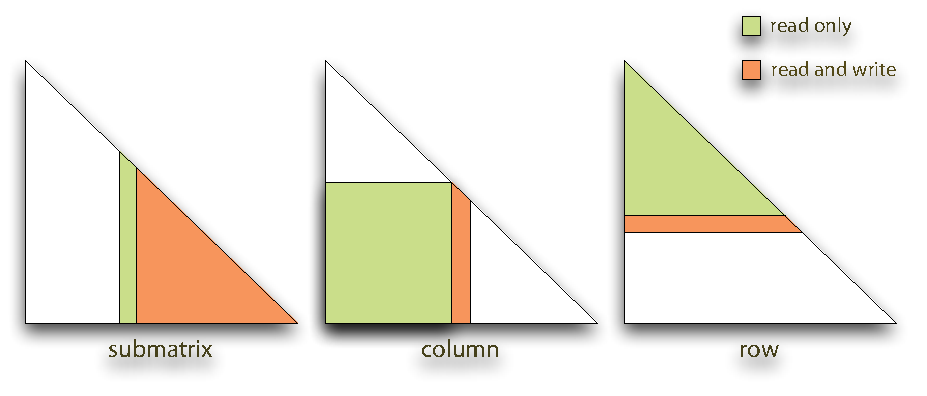
\includegraphics[scale=0.7]{figures/cholesky-memory.pdf}
  \end{figure}
%
\end{frame}

% end of file 

% -*- LaTeX -*-
% -*- coding: utf-8 -*-
%
% ~~~~~~~~~~~~~~~~~~~~~~~~~~~~~~~~~~~~~~~~~~~~~~~~~~~~~~~~~~~~~~~~~~~~~~~~~~~~~~
%
%                             michael a.g. aïvázis
%                      california institute of technology
%                      (c) 1998-2010  all rights reserved
%
% ~~~~~~~~~~~~~~~~~~~~~~~~~~~~~~~~~~~~~~~~~~~~~~~~~~~~~~~~~~~~~~~~~~~~~~~~~~~~~~
%

\lecture{Matrices}{20100305}

% --------------------------------------
% LU factorization
\begin{frame}[fragile]
%
  \frametitle{$LU$ factorization}
%
  \begin{itemize}
%
  \item systems of linear equations are ubiquitous in numerical analysis
  \item let $A$ be an $n \times n$ matrix, $b$ a known $n$-vector; we are looking for $x$ such
    that
    \begin{equation}
      A x = b \label{eq:linear-system}
    \end{equation}
  \item a commonly used direct method for solving this system is to convert $A$ into the
    product of a lower triangular matrix $L$ with an upper triangular matrix $U$
    \begin{equation}
      A = L U \label{eq:LU-factorization}
    \end{equation}
    known as $LU$ factorization
  \item \eqref{linear-system} becomes
    \begin{equation}
      L U x = b
    \end{equation}
    which we can now solve in two simpler steps
    \begin{eqnarray}
        L y & = & b \\
        U x & = & y
    \end{eqnarray}
    where we first solve the lower triangular system by forward substitution, followed by
    solving the upper triangular system by back substitution to obtain $x$
%
  \end{itemize}
%
\end{frame}

% --------------------------------------
% LU by Gaussian elimination
\begin{frame}[fragile]
%
  \frametitle{$LU$ by Gaussian elimination}
%
  \begin{itemize}
%
  \item we can compute the $LU$ factorization of $A$ using Gaussian elimination
    \begin{center}
      \begin{minipage}{.85\linewidth}
        \begin{algorithm}[H]
          \label{alg:LU-gaussian}
%
          \DontPrintSemicolon
          % \NoCaptionOfAlgo
          \SetAlCapHSkip{0ex}
%
          \caption{\lu(A)}
%
          \For{$k=1$ \KwTo $n-1$}{
            \For{$i=k+1$ \KwTo $n$}{
              $L_{ik} = A_{ik} / A_{kk}$
            }
            \For{$j=k+1$ \KwTo $n$}{
              \For{$i=k+1$ \KwTo $n$}{
                $A_{ij} = A_{ij} - L_{ik}A_{kj}$
              }
            }
          }
%
        \end{algorithm}
      \end{minipage}
    \end{center}
%
    which encodes $L$ and $U$ in place by overwriting $A$
%
  \item \algref{LU-gaussian} requires roughly $n^{3}/3$ multiply-adds and $n^{2}/2$ divisions
%
  \item we may also need {\em pivoting} to ensure numerical stability (and existence)
%
  \item \algref{LU-gaussian} is one of many algorithms expressed essentially as a triply nested loop
    \begin{itemize}
    \item the three indices can be ordered in any of $3!$ ways, with totally different memory
      access patterns
    \item in parallel, the $kij$ and $kji$ forms may be the most efficient
    \end{itemize}
%
  \end{itemize}
%
\end{frame}
%

% --------------------------------------
% parallelization strategy
\begin{frame}[fragile]
%
  \frametitle{Parallel $LU$ decomposition}
%
  \begin{itemize}
%
  \item number fine grain tasks as $(i,j)$ with $i,j = 1, \ldots, n$; each task
    \begin{itemize}
    \item stores $A_{ij}$
    \item computes and stores $U_{ij}$, if $i \leq j$
    \item computes and stores $L_{ij}$, if $i > j$
    \end{itemize}
    yielding a two dimensional array of $n^{2}$ tasks
%
  \item no need to compute and store
    \begin{itemize}
    \item the zeroes in the lower triangle of $U$
    \item the unit diagonal and the zeroes in the upper triangle of $L$
    \end{itemize}
%
  \item in order to create $p$ coarse grain tasks we could combine
    \begin{itemize}
    \item $n/p$ rows or columns of fine grain tasks
    \item $(n/\sqrt{p}) \times (n/\sqrt{p})$ blocks of tasks
    \end{itemize}
    and map each one to a process
%
  \end{itemize}
% 
\end{frame}

% --------------------------------------
% parallelization LU
\begin{frame}[fragile]
%
  \frametitle{Communication patterns for parallel $LU$ decomposition}
%
  \begin{center}
    \begin{minipage}{.85\linewidth}
      \begin{algorithm}[H]
        \label{alg:pLU-ij}
%
        \DontPrintSemicolon
        % \NoCaptionOfAlgo
        \SetAlCapHSkip{0ex}
%
        \caption{\lu($A$, task=$(i,j)$)}
%
        \For{$k=1$ \KwTo $\min(i,j) - 1$}{
          \KwRecv $A_{kj}$ \;
          \KwRecv $L_{ik}$ \;
          $A_{ij} = A_{ij}- L_{ik}A_{kj}$
        }
        \If{ $i \leq j$}{
          \KwBcast $A_{ij}$ \KwTo $(k,j)$, $k=i+1,\ldots,n$
        } \Else {
          \KwRecv $A_{jj}$ \;
          $L_{ij} = A_{ij}/A_{jj}$ \;
          \KwBcast $L_{ij}$ \KwTo $(i,k)$, $k=i+1,\ldots,n$
        }
% 
      \end{algorithm}
    \end{minipage}
  \end{center}
%
\end{frame}

% --------------------------------------
% row coarsening
\begin{frame}[fragile]
%
  \frametitle{Row coarsening}
%
  \begin{itemize}
%
  \item with one dimensional row coarsening
    \begin{itemize}
    \item we forgo parallelism in updating rows
    \item there is no need to broadcast the multipliers $L_{ij}$ since each row is contained
      entirely within a task
    \item we still need the vertical broadcasts of matrix rows to the tasks below
    \end{itemize}
%
  \end{itemize}
%
  \begin{center}
    \begin{minipage}{.85\linewidth}
      \begin{algorithm}[H]
        \label{alg:pLU-ij-rows}
%
        \DontPrintSemicolon
        % \NoCaptionOfAlgo
        \SetAlCapHSkip{0ex}
%
        \caption{\lu($A$, task=$(i,j)$) by rows}
%
        \For{$k=1$ \KwTo $n - 1$}{
          \If{ $k \in myrows$}{
            \KwBcast $\left\{A_{kj} : k\leq j  \leq n\right\}$
          } \Else {
            \KwRecv $\left\{A_{kj} : k\leq j  \leq n\right\}$
          }
          \For{$i \in myrows$, $i > k$} {
            $L_{ik} = A_{ik}/ A_{kk}$
          }
          \For{$j=k+1$ \KwTo $n$}{
            \For{ $i \in myrows$, $i>k$}{
              $A_{ij} = A_{ij} - L_{ik} A_{kj}$
            }
          }
        }
% 
      \end{algorithm}
    \end{minipage}
  \end{center}
% 
\end{frame}

% --------------------------------------
% observations
\begin{frame}[fragile]
%
  \frametitle{Observations on row coarsening}
%
  \begin{itemize}
%
  \item each task becomes idle as soon as it last row is completed
    \begin{itemize}
    \item if rows are contiguous, a task may finish long before the overall computation is done
    \item even worse, updating rows requires progressively less work with increasing row number
    \end{itemize}
%
  \item we may improve concurrency and load balance 
    \begin{itemize}
    \item by assigning rows to tasks in a cyclic manner where row $i$ is updated by task $i
      \mod p$
    \item other mappings may be useful
    \end{itemize}
%
  \item other improvements involve overlapping computation with communication
    \begin{itemize}
    \item at step $k$, each task completes updating its portion of the remaining unreduced
      matrix before moving on to step $k+1$
    \item however, the task that owns the $k+1$ row could broadcast it as soon as it becomes
      available, before moving on to the step $k$ update
    \item this {\em send ahead} strategy may grant other tasks earlier access to the data
      necessary to start working on the next step
    \end{itemize}
%
  \end{itemize}
%
\end{frame}

% --------------------------------------
% column coarsening
\begin{frame}[fragile]
%
  \frametitle{Column coarsening}
%
  \begin{center}
    \begin{minipage}{.85\linewidth}
      \begin{algorithm}[H]
        \label{alg:pLU-ij-columns}
%
        \DontPrintSemicolon
        % \NoCaptionOfAlgo
        \SetAlCapHSkip{0ex}
%
        \caption{\lu($A$, task=$(i,j)$) by columns}
%
        \For{$k=1$ \KwTo $n - 1$}{
          \If{ $k \in mycolumns$}{
            \For{ $i=k+1$ \KwTo $n$}{
              $L_{ik} = A_{ik}/ A_{kk}$
            }
            \KwBcast $\left\{L_{ik} : k < i  \leq n\right\}$
          } \Else {
            \KwRecv $\left\{L_{ik} : k < i  \leq n\right\}$
          }
          \For{$i \in mycolumns$, $j > k$} {
            \For{$i=k+1$ \KwTo $n$}{
              $A_{ij} = A_{ij} - L_{ik} A_{kj}$
            }
          }
        }
% 
      \end{algorithm}
    \end{minipage}
  \end{center}
%
  \begin{itemize}
  \item observations similar to row coarsening apply
  \end{itemize}
% 
\end{frame}

% --------------------------------------
% column coarsening
\begin{frame}[fragile]
%
  \frametitle{Block coarsening}
%
  \begin{center}
      \begin{algorithm}[H]
        \label{alg:pLU-ij-blocks}
%
        \DontPrintSemicolon
        % \NoCaptionOfAlgo
        \SetAlCapHSkip{0ex}
%
        \caption{\lu($A$, task=$(i,j)$) by blocks}
%
        \For{$k=1$ \KwTo $n - 1$}{
          \If{$k \in myrows$}{
            \KwBcast $\left\{A_{kj} : j \in mycolumns, j>k\right\}$ \KwTo 
            all tasks in my task column
          } \Else {
            \KwRecv $\left\{A_{kj} : j \in mycolumns, j>k\right\}$
          }
          \If{$k \in mycolumns$}{
            \For{$i \in myrows$, $i>k$}{
              $L_{ik} = A_{ik} / A_{kk}$
            }
            \KwBcast $\left\{L_{ik} : i \in myrows, i>k\right\}$ \KwTo 
            all tasks in my task row
          } \Else {
            \KwRecv $\left\{L_{ik} : i \in myrows, i>k\right\}$
          }
          \For{$j \in mycolumns$, $j>k$}{
            \For{$i \in myrows$, $i>k$} {
              $A{ij} = A_{ij} - L_{ik}A_{kj}$
            }
          }
        }
% 
      \end{algorithm}
  \end{center}
%
\end{frame}

% --------------------------------------
% observations
\begin{frame}[fragile]
%
  \frametitle{Observations on block coarsening}
%
  \begin{itemize}
%
  \item each task becomes idle as soon as it last row and column are completed
    \begin{itemize}
    \item if rows and columns are in contiguous blocks, a task may finish long before the
      overall computation is done
    \item even worse, computing multipliers and updating blocks requires progressively less
      work with increasing row and column numbers
    \end{itemize}
%
  \item we may improve concurrency and load balance 
    \begin{itemize}
    \item by assigning rows and columns to tasks in a cyclic manner where $A_{ij}$ is assigned
      to task $(i \mod \sqrt{p}, j \mod \sqrt{p}$
    \item other mappings may be useful
    \end{itemize}
%
  \item other improvements involve overlapping computation with communication
    \begin{itemize}
    \item at step $k$, each task completes updating its portion of the remaining unreduced
      submatrix before moving on to step $k+1$
    \item the broadcast of each segment of row $k+1$, and the computation and broadcast of each
      segment of multipliers for step $k+1$, can be initiated as soon as the relevant segments
      of row $k+1$ and column $k+1$ have been updated by their owners, before moving to
      competing the update for step $k$
    \item this {\em send ahead} strategy may grant other tasks earlier access to the data
      necessary to start working on the next step
    \end{itemize}
%
  \end{itemize}
%
\end{frame}

% --------------------------------------
% pivoting
\begin{frame}[fragile]
%
  \frametitle{Pivoting}
%
  \begin{itemize}
%
  \item the order of rows of $A$ does not affect the solution to the system of equations
    \begin{itemize}
    \item {\em partial pivoting} sorts the rows by the largest absolute value of the leading
      column of the remaining unreduced matrix
    \item this choice ensures that the magnitude of the multipliers do not exceed 1, which
      \begin{itemize}
      \item reduces amplification of round-off errors
      \item ensures existence
      \item improves numerical stability
      \end{itemize}
    \end{itemize}
%
  \item partial pivoting introduces a permutation matrix $P$, which leads to the factorization
    \begin{equation}
      P A = L U
    \end{equation}
    which implies that the solution $x$ is obtained through
    \begin{eqnarray}
      L y & = & P b \\
      U x & = & y
    \end{eqnarray}
    with forward substitution in the lower triangular system, followed by back substitution in
    the upper triangular system
%
  \end{itemize}
%
\end{frame}

% --------------------------------------
% parallel pivoting
\begin{frame}[fragile]
%
  \frametitle{Pivoting in parallel}
%
  \begin{itemize}
%
  \item increased numerical stability costs increased parallel complexity and significant
    performance implications
  \item for one dimensional coarsening by column, the search for the pivot element requires no
    extra communication, but it is purely serial
    \begin{itemize}
    \item once the pivot is found, the index of the pivot row must be communicated to the other
      tasks, and rows must be explicitly or implicitly interchanged in each task
    \end{itemize}
  \item for coarsening by rows, the search for the pivot is parallel, but it requires
    communication among tasks and inhibits the overlapping of successive steps
    \begin{itemize}
    \item if rows are explicitly interchanged, then only two tasks are involved
    \item if rows are implicitly interchanged, changes to the assignment of rows to tasks are
      required, which has effects on concurrency and load balance
    \end{itemize}
  \item in the presence of partial pivoting, column and row coarsening trade off on the
    relative speeds of computation versus communication
%
  \item with two dimensional coarsening, pivot search is parallel but requires communication
    among tasks along columns and destroys the possibility of overlapping successive steps
%
  \end{itemize}
%
\end{frame}

% --------------------------------------
% pivoting alternatives
\begin{frame}[fragile]
%
  \frametitle{Alternatives to pivoting}
%
  \begin{itemize}
%
  \item various alternatives have been proposed
    \begin{itemize}
    \item constraining pivoting to blocks of rows
    \item pivoting when the multiplier exceeds a given threshold
    \item pairwise pivoting 
    \end{itemize}
%
  \item these strategies are not foolproof, and trade off some stability and accuracy for speed
%
  \end{itemize}
%
\end{frame}

% --------------------------------------
% cholesky
\begin{frame}[fragile]
%
  \frametitle{Cholesky factorization}
%
  \begin{itemize}
%
  \item when $A$ is a positive definite symmetric matrix is has a Cholesky factorization
    \begin{equation}
      A = L L^{T}
    \end{equation}
    with $L$ a lower triangular matrix with positive entries along the diagonal
%
  \item so the linear system $Ax=b$ can be solved through
    \begin{eqnarray}
      L y & = & b \\
      L^{T} x & = & y 
    \end{eqnarray}
%
  \item the factorization is derived by equating corresponding entries of $A$ with those of $L
    L^{T}$ and generating them in the correct order
    \begin{itemize}
    \item for example, in the $2 \times 2$ case
      \begin{equation}
        \left[
          \begin{array}{cc}
            A_{11} & A_{21} \\
            A_{21} & A_{22}
          \end{array}
        \right]
        =
        \left[
          \begin{array}{cc}
            L_{11} & 0 \\
            L_{21} & L_{22}
          \end{array}
        \right]
        \left[
          \begin{array}{cc}
            L_{11} & L_{21} \\
            0 & L_{22}
          \end{array}
        \right]
      \end{equation}
      yields
      \begin{eqnarray}
        L_{11} = \sqrt{A_{11}} & 
        L_{21} = A_{21}/L_{11} & 
        L_{22} = \sqrt{A_{22} - L_{21}^{2}}
      \end{eqnarray}
      

    \end{itemize}
% 
  \end{itemize}
%
\end{frame}

% --------------------------------------
% implementation of cholesky
\begin{frame}[fragile]
%
  \frametitle{Computing the Cholesky factorization}
%
    \begin{center}
      \begin{minipage}{.85\linewidth}
        \begin{algorithm}[H]
          \label{alg:cholesky}
%
          \DontPrintSemicolon
          % \NoCaptionOfAlgo
          \SetAlCapHSkip{0ex}
%
          \caption{\cholesky(A)}
%
          \For{$k=1$ \KwTo $n$}{
            $A_{kk} = \sqrt{A_{kk}}$ \;
            \For{$i=k+1$ \KwTo $n$}{
              $A_{ik} = A_{ik} / A_{kk}$
            }
            \For{$j=k+1$ \KwTo $n$}{
              \For{$i=j$ \KwTo $n$}{
                $A_{ij} = A_{ij} - A_{ik}A_{jk}$
              }
            }
          }
%
        \end{algorithm}
      \end{minipage}
    \end{center}
%
  \begin{itemize}
%
  \item note that
    \begin{itemize}
    \item $n$ square roots are required, all of positive numbers 
    \item only lower triangle of $A$ is accessed, so the strict upper triangular part need not
      be stored
    \item $A$ becomes $L$ in place
    \item the algorithm is stable so no pivoting is required
    \end{itemize}
%
  \item it takes roughly half the number of $LU$ operations: approximately $n^{3}/6$
    multiply-adds
  \end{itemize}
%
\end{frame}

% --------------------------------------
% parallel cholesky
\begin{frame}[fragile]
%
  \frametitle{Parallelizing Cholesky}
%
  \begin{itemize}
%
  \item number fine grain tasks as $(i,j)$ with $i,j = 1, \ldots, n$; each task
    \begin{itemize}
    \item stores $A_{ij}$
    \item computes and stores $L_{ij}$, if $i \geq j$
    \item computes and stores $L_{ji}$, if $i < j$
    \end{itemize}
    yielding a two dimensional array of $n^{2}$ tasks
%
  \item no need to compute and store the zero entries in the upper triangle
%
  \end{itemize}
%
\end{frame}

% --------------------------------------
% communication patterns for parallel cholesky
\begin{frame}[fragile]
%
  \frametitle{Communication patterns for parallel Cholesky}
%
  \begin{center}
    \small
    \begin{minipage}{.85\linewidth}
      \begin{algorithm}[H]
        \label{alg:pCholesky}
%
        \DontPrintSemicolon
        % \NoCaptionOfAlgo
        \SetAlCapHSkip{0ex}
%
        \caption{\cholesky($A$, task=$(i,j)$)}
%
        \For{$k=1$ \KwTo $\min(i,j) - 1$}{
          \KwRecv $A_{kj}$ \;
          \KwRecv $A_{ik}$ \;
          $A_{ij} = A_{ij}- A_{ik}A_{kj}$
        }
        \If{$i = j$}{
          $A_{ii} = \sqrt{A_{ii}}$ \;
          \KwBcast $A_{il}$ \KwTo tasks $(k,i)$ and $(i,k)$, $k=i+1,\ldots,n$
        } 
        \If {$i < j$}{
          \KwRecv $A_{ii}$ \;
          $A_{ij} = A_{ij}/A_{ii}$ \;
          \KwBcast $A_{ij}$ \KwTo $(k,j)$, $k=i+1,\ldots,n$
        }
        \If {$i > j$} {
          \KwRecv $A_{jj}$ \;
          $A_{ij} = A_{ij}/A_{jj}$ \;
          \KwBcast $A_{ij}$ \KwTo $(i,k)$, $k=j+1,\ldots,n$
        }
% 
      \end{algorithm}
    \end{minipage}
  \end{center}
%
\end{frame}

% --------------------------------------
% coarsening
\begin{frame}[fragile]
%
  \frametitle{Coarsening}
%
  \begin{itemize}
%
  \item strategies very similar to $LU$ factorization
    \begin{itemize}
    \item one dimensional by row or column
    \item two dimensional blocks
    \end{itemize}
    with column coarsening used most often in practice
%
  \item each choice of index in the outer loop yields different algorithm, named after the
    portion of the matrix that is updated by the basic operation in the inner loops
%
    \begin{itemize}
    \item submatrix Cholesky: with $k$ as the outer loop index, the inner loops perform a rank
      1 update of the remaining unreduced submatrix, using the current column
    \item column Cholesky: with $j$ in the outer loop, inner loops compute the current column,
      using matrix-vector multiplies that accumulates the effects of previous columns
    \item row Cholesky: with $i$ in the outer loop, inner loops compute current row by solving
      a triangular system involving the previous rows
    \end{itemize}
%
  \end{itemize}
%
\end{frame}


% --------------------------------------
% memory access patterns
\begin{frame}[fragile]
%
  \frametitle{Cholesky memory access patterns}
%
  \begin{figure}
    \centering
    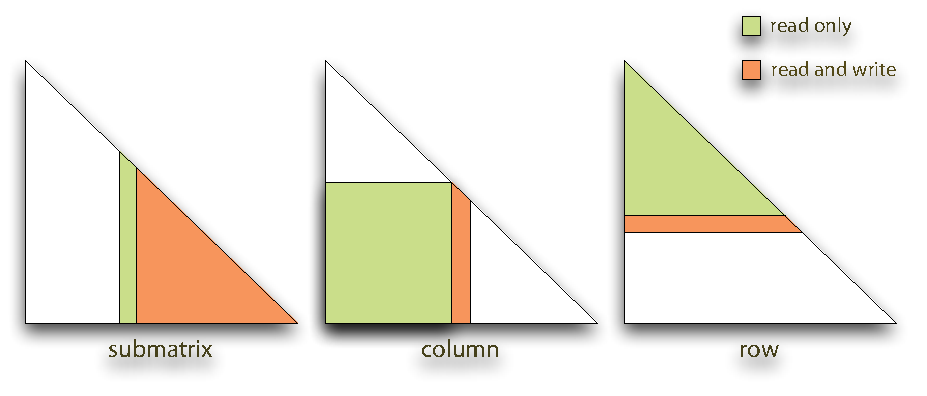
\includegraphics[scale=0.7]{figures/cholesky-memory.pdf}
  \end{figure}
%
\end{frame}

% end of file 

% -*- LaTeX -*-
% -*- coding: utf-8 -*-
%
% ~~~~~~~~~~~~~~~~~~~~~~~~~~~~~~~~~~~~~~~~~~~~~~~~~~~~~~~~~~~~~~~~~~~~~~~~~~~~~~
%
%                             michael a.g. aïvázis
%                      california institute of technology
%                      (c) 1998-2010  all rights reserved
%
% ~~~~~~~~~~~~~~~~~~~~~~~~~~~~~~~~~~~~~~~~~~~~~~~~~~~~~~~~~~~~~~~~~~~~~~~~~~~~~~
%

\lecture{Matrices}{20100308}

% --------------------------------------
% triangular systems
\begin{frame}[fragile]
%
  \frametitle{Triangular systems}
%
  \begin{itemize}
%
  \item a matrix $L$ is lower triangular if all entries above the main diagonal are zero: $L_{ij} =
    0$ for $i < j$.
  \item a matrix $U$ is upper triangular if all entries below the main diagonal are zero: $U_{ij} =
    0$ for $i > j$.
  \item triangular systems appear frequently
    \begin{itemize}
    \item most direct methods of solving linear systems of equation start with a reduction of
      the matrix of coefficients into triangular form
    \item they are also used as preconditioners in iterative methods
    \end{itemize}
%
  \end{itemize}
%
\end{frame}

% --------------------------------------
% forward substitution
\begin{frame}[fragile]
%
  \frametitle{Forward substitution}
%
  \begin{itemize}
%
  \item the lower triangular system $Lx = b$ can be solved by {\em forward substitution}
    \begin{equation}
      x_{i} = \left( b_{i} - \sum_{j=1}^{i-1} L_{ij}x_{j} \right) / L_{ii}
    \end{equation}
%
  \item that can be implemented as
    \begin{center}
      \begin{minipage}{.85\linewidth}
        \begin{algorithm}[H]
          \label{alg:forward-substitution}
%
          \DontPrintSemicolon
          % \NoCaptionOfAlgo
          \SetAlCapHSkip{0ex}
%
          \caption{\forwsub(L, b)}
%
          \For{$j=1$ \KwTo $n$}{
            $x_{j} = b_{j} / L_{jj}$ \;
            \For{$i=j+1$ \KwTo $n$}{
              $b_{i} = b_{i} - L_{ij} x_{j}$
            }
          }
%
        \end{algorithm}
      \end{minipage}
    \end{center}
%
  \item with roughly $n^{2}$ multiply-adds
%
  \end{itemize}
%
\end{frame}

% --------------------------------------
% backward substitution
\begin{frame}[fragile]
%
  \frametitle{Backward substitution}
%
  \begin{itemize}
%
%
  \item the upper triangular system $Ux = b$ can be solved by {\em backward substitution}
    \begin{equation}
      x_{i} = \left( b_{i} - \sum_{j=i+1}^{n} U_{ij}x_{j} \right) / U_{ii}
    \end{equation}
%
  \item that can be implemented as
    \begin{center}
      \begin{minipage}{.85\linewidth}
        \begin{algorithm}[H]
          \label{alg:backward-substitution}
%
          \DontPrintSemicolon
          % \NoCaptionOfAlgo
          \SetAlCapHSkip{0ex}
%
          \caption{\backsub(L, b)}
%
          \For{$j=n$ \KwTo $1$}{
            $x_{j} = b_{j} / U_{jj}$ \;
            \For{$i=1$ \KwTo $j-1$}{
              $b_{i} = b_{i} - U_{ij} x_{j}$
            }
          }
%
        \end{algorithm}
      \end{minipage}
    \end{center}
%
  \item with roughly $n^{2}$ multiply-adds
%
  \item the two algorithms are very similar, so focus on lower triangular systems
%
  \end{itemize}
%
\end{frame}

% --------------------------------------
% sequential implementations
\begin{frame}[fragile]
%
  \frametitle{Sequential implementations}
%
  \begin{itemize}
  \item there are two possible ways to arrange the forward substitution loops 
  \end{itemize}
%
  \begin{minipage}{.45\linewidth}
    \small
    \begin{algorithm}[H]
%
      \DontPrintSemicolon
      \NoCaptionOfAlgo
%
      \For{$j=1$ \KwTo $n$}{
        $x_{j} = b_{j} / L_{jj}$ \;
        \For{$i=j+1$ \KwTo $n$}{
          $b_{i} = b_{i} - L_{ij} x_{j}$
        }
      }
%
    \end{algorithm}
%
    \begin{itemize}
    \item immediate update
    \item data driven
    \item fan out
    \end{itemize}
%
  \end{minipage}
%
  \hfill
%
  \begin{minipage}{.45\linewidth}
    \small
    \begin{algorithm}[H]
%
      \DontPrintSemicolon
      \NoCaptionOfAlgo
%
      \For{$i=1$ \KwTo $n$}{
        \For{$j=1$ \KwTo $i-1$}{
          $b_{i} = b_{i} - L_{ij} x_{j}$
        }
        $x_{i} = b_{i} / L_{ii}$ \;
      }
%
    \end{algorithm}
%
    \begin{itemize}
    \item delayed update
    \item demand driven
    \item fan in
    \end{itemize}
%
  \end{minipage}
%
\end{frame}

% --------------------------------------
% parallelization
\begin{frame}[fragile]
%
  \frametitle{Parallelization}
%
  \begin{itemize}
%
  \item label the fine grain tasks as $(i,j)$ with $i,j = 1,\ldots,n$
    \begin{itemize}
    \item for $i=2,\ldots,n$ and $j=1,\ldots,i-1$, task $(i,j)$
      \begin{itemize}
      \item stores $L_{ij}$ 
      \item computes $L_{ij} x_{j}$
      \end{itemize}
    \item for $i=1,\ldots,n$, task $(i,i)$
      \begin{itemize}
      \item stores $L_{ii}$ and $b_{i}$
      \item collects the sum $t_{i} = \sum_{j=1}^{i-1} L_{ij}x_{j}$
        \item computes and stores $x+{i} = (b_{i} - t_{i})/ L_{ii}$
      \end{itemize}
    \end{itemize}
%
    \item this arrangement yields a two dimensional triangular grid of $n(n+1)/2$ fine grain tasks
%
    \item with the following communication patterns
      \begin{itemize}
      \item for $j=1,\ldots,n-1$, task $(j,j)$ broadcasts $x_{j}$ to tasks $(i,j)$,
        $i=j+1,\ldots,n$ 
      \item for $i=1,\ldots,n$, task $(i,i)$ collects the sum reduction of $L_{ij} x_{j}$ from
        tasks $(i,j)$, $j=1,\ldots,i-1$
      \end{itemize}
  \end{itemize}
%
\end{frame}

% --------------------------------------
% parallel implementation
\begin{frame}[fragile]
%
  \frametitle{Parallel implementation}
%
  \begin{itemize}
  \item here is the program for task $(i,j)$ with $i \geq j$
%
  \begin{center}
    \footnotesize
    \begin{minipage}{.85\linewidth}
      \begin{algorithm}[H]
%
        \DontPrintSemicolon
        \NoCaptionOfAlgo
        \SetAlCapHSkip{0ex}
%
        \If{$i = j$}{
          \If{$i > 1$}{
            \KwRecv sum reduction $t$ \;
          } \Else {
            $t = 0$
          }
          \KwBcast $x_{i}$ \KwTo tasks $(k,i)$ and $(i,k)$, $k=i+1,\ldots,n$
        } \Else {
          \KwRecv $x_{j}$ \;
          $t = L_{ij} x_{j}$ \;
          \KwSend $t$ for reduction across tasks $(i,k)$, $k=1,\ldots,i-1$ to task $(i,i)$\;
        }
% 
      \end{algorithm}
    \end{minipage}
  \end{center}
%
  \item for properly pipelined communication, this algorithm can be implemented in $\order{n}$,
    but it requires $\order{n^{2}}$ tasks
  \item if there are many $b$ to solve for, the tasks can be working on multiple systems at
    the same time
  \item coarsening strategies can manage the number of tasks and improve the balance between
    computation and communication
  \end{itemize}
%
\end{frame}

% --------------------------------------
% coarsening
\begin{frame}[fragile]
%
  \frametitle{Coarsening by rows}
%
  \begin{itemize}
%
  \item for one dimensional coarsening into $n/p$ rows
    \begin{itemize}
    \item there is no need to communicate to perform the reductions, but also no parallelism
    \item vertical broadcasts are still needed to move the components of $x$
    \end{itemize}
%
  \begin{center}
    \begin{minipage}{.85\linewidth}
      \begin{algorithm}[H]
%
        \DontPrintSemicolon
        \NoCaptionOfAlgo
        \SetAlCapHSkip{0ex}
%
        \For{$j=1$ \KwTo $n$}{
          \If{ $j \in myrows$}{
            $x_{j} = b_{j} / L_{jj}$ \;
            \KwBcast $x_{j}$ to other tasks \;
          } \Else {
            \KwRecv $x_{j}$
          }
          \For{$i \in myrows$, $i > j$} {
            $b_{i} = b_{i} - L_{ij}/ x_{j}$
          }
        }
% 
      \end{algorithm}
    \end{minipage}
  \end{center}
%
  \end{itemize}
%
\end{frame}

% --------------------------------------
% coarsening by columns
\begin{frame}[fragile]
%
  \frametitle{Observations on coarsening by rows}
%
  \begin{itemize}
%
  \item load balance:
%
    \begin{itemize}
    \item tasks become idle after the solution components corresponding to their last row are
      computed, and there is progressively more work as row number increases
    \item if a task holds a contiguous block of rows, it may become idle before mush of the
      calculation is finished
    \end{itemize}
%
  \item both concurrency and load balance may be improved by assigning rows to tasks in more
    creative ways
    \begin{itemize}
    \item cyclically: assign row $j$ to task $j \mod p$
    \item block cyclically
    \item reflectively
    \end{itemize}
%
  \item overall execution speed depends on the ability to overlap communication with the
    computation of successive steps
%
  \end{itemize}
%
\end{frame}

% --------------------------------------
% coarsening by columns
\begin{frame}[fragile]
%
  \frametitle{Coarsening by columns}
%
  \begin{itemize}
%
  \item for one dimensional coarsening into $n/p$ rows
    \begin{itemize}
    \item there is no need to broadcast the components of $x$ vertically, but also no
      parallelism in computing the products
    \item horizontal exchanges are still required for the sum reductions that accumulate the
      inner products
    \end{itemize}
%
  \begin{center}
    \begin{minipage}{.85\linewidth}
      \begin{algorithm}[H]
%
        \DontPrintSemicolon
        \NoCaptionOfAlgo
        \SetAlCapHSkip{0ex}
%
        \For{$i=1$ \KwTo $n$}{
          t = 0 \;
          \For{ $j \in mycolumns$, $j < i$}{
            $t = t + L_{ij} x_{j}$
          }
          \If{ $i \in mycolumns$} {
            \KwRecv reduction of $t$ \;
            $x_{i} = (b_{i} -t)/ L_{ii}$
          } \Else {
            \KwSend $t$ for reduction across all tasks
          }
        }
% 
      \end{algorithm}
    \end{minipage}
  \end{center}
%
  \end{itemize}
%
\end{frame}

% --------------------------------------
% observations on coarsening by columns
\begin{frame}[fragile]
%
  \frametitle{Observations on coarsening by columns}
%
  \begin{itemize}
%
%
  \item load balance:
    \begin{itemize}
    \item tasks are idle until solution component corresponding to their first column is
      computed, and there is progressively less work as column number increases
    \item if a task holds a contiguous block of columns, it may remain idle for most of the
      calculation
    \end{itemize}
%
  \item both concurrency and load balance may be improved by assigning columns to tasks in more
    creative ways
    \begin{itemize}
    \item cyclically: assign column $j$ to task $j \mod p$
    \item block cyclically
    \item reflectively
    \end{itemize}
%
  \item overall execution speed depends on the ability to overlap communication with the
    computation of successive steps
%
  \end{itemize}
%
\end{frame}

% --------------------------------------
% wavefront algorithms
\begin{frame}[fragile]
%
  \frametitle{Wavefront algorithms}
%
  \begin{itemize}
%
  \item fan out and fan in algorithm share many characteristics
    \begin{itemize}
    \item parallelism comes from partitioning and distributing the work of the inner loop
    \item while the outer loop is serial
    \item they work on one component of the solution at a time, although one can partially
      pipeline successive steps
    \end{itemize}
%
    \item {\em wavefront} algorithms exploit parallelism in the outer loops by explicitly
      working on multiple components of the solution at the same time
%
    \item consider the one dimensional fan out algorithm
      \begin{itemize}
      \item it appears there is no opportunity for parallelism: after the owner of column $j$
        computes $x_{j}$, the updated components of $b$ cannot shared with other tasks because
        they have no access to column $j$
      \item however, the task that owns column $j$ could finish only a fraction of the work,
        say the first $s$ components, and pass them on to the task that owns column $j+1$,
        before continuing on to the next $s$ components
      \item the task that owns column $j+1$ receives the first $s$ components of $b$, it can
        compute $x_{j+1}$, begin a fraction of the remaining updates and forward its
        contributions to the next task
      \end{itemize}
%
  \end{itemize}
%
\end{frame}

% --------------------------------------
% wavefront implementation
\begin{frame}[fragile]
%
  \frametitle{Wavefront implementation}
%
  \begin{itemize}
%
  \item we need two new features
    \begin{itemize}
    \item a vector $z$ that accumulates the updates to $b$
    \item the notion of a {\em segment} that contains no more than $s$ consecutive components of $z$
    \end{itemize}
%
  \end{itemize}
%
  \begin{center}
    \begin{minipage}{.85\linewidth}
      \begin{algorithm}[H]
%
          \DontPrintSemicolon
          \NoCaptionOfAlgo
          \SetAlCapHSkip{0ex}
%
          \For{$j \in mycolumns$}{
            \For{$k=1$ \KwTo number of segments}{
              \KwRecv $segment$\;
              \If {$k=1$} {
                $x_{j} = (b_{j} - z_{j})/ L_{jj}$ \;
                $segment = segment - \{z_{j}\}$ \;
              }
              \For{$z_{i} \in segment$} {
                $z_{i} = z_{i} + L_{ij}x_{j}$ \;
              }
              \If{$length(segment) > 0$}{
                \KwSend $segment$ \KwTo task owning column $j+1$
              }
            }
          }
%
        \end{algorithm}
      \end{minipage}
    \end{center}
%
\end{frame}



% --------------------------------------
% two dimensional coarsening
\begin{frame}[fragile]
%
  \frametitle{Block coarsening}
%
  \begin{itemize}
%
  \item coalesce $(n/\sqrt{p}) \times (n/\sqrt{p})$ fine grain tasks in to a coarse grain block
%
  \item resulting in an algorithm with features from both column and row coarsening
    \begin{itemize}
    \item both vertical broadcasts and horizontal reductions are required to communicate
      solution components and accumulate inner products
    \end{itemize}
%
  \item the na\"ive implementation assigns contiguous blocks of rows and columns to coarse
    tasks
    \begin{itemize}
    \item poor concurrency and efficiency 
    \item almost half the tasks are idle
    \end{itemize}
%
  \item cyclic assignment, with $L_{ij}$ assigned to task $(i \mod \sqrt{p}, j \mod \sqrt{p})$,
    yields $p$ non-null tasks so the full grid of tasks is active
    \begin{itemize}
    \item again, the obvious implementation where we loop over successive solution components
      to perform horizontal reductions and vertical broadcasts has limited concurrency, since
      computation of each component involves only one task row and one task column
    \item improve by computing solution components in groups of $\sqrt{p}$, which enables all
      tasks to perform the updates concurrently
    \end{itemize}
%
  \end{itemize}
%
\end{frame}

% --------------------------------------
% iterative methods
\begin{frame}[fragile]
%
  \frametitle{Iterative methods}
%
  \begin{itemize}
%
  \item iterative methods start with an initial guess for the vector $x$ and improve until some
    desired accuracy is achieved
    \begin{itemize}
    \item no upper bound on the number of iterations to the exact solution
    \item in practice, establish an error measure such as $||b - Ax|| < \epsilon$
    \item particularly good with sparse matrices because sparsity is preserved
    \end{itemize}
  \item we will take a quick look at
    \begin{itemize}
    \item Jacobi
    \item Gauss-Seidel
    \item successive over-relaxation (SOR)
    \item conjugate gradient
    \end{itemize}
%
  \end{itemize}
%
\end{frame}

% --------------------------------------
% template
\begin{frame}[fragile]
%
  \frametitle{The Jacobi method}
%
  \begin{itemize}
%
  \item given an initial guess $x^{(0)}$, the Jacobi method iterates by
    \begin{equation}
      x_{i}^{(k+1)} = \left( b_{i} - \sum_{j\neq i} A_{ij}x_{j}^{(k)} \right) / A_{ii}
    \end{equation}
    which can be expressed as
    \begin{equation}
      x^{(k+1)} = D^{-1} \left( b - (L+U)x^{(k)} \right)
    \end{equation}
    for $D$, $L$, and $U$ respectively diagonal, upper and lower triangular matrices
%
    \item the method requires
      \begin{itemize}
      \item non-zero diagonal entries, usually achievable by permuting rows
      \item extra storage for the $x$ iterates
      \end{itemize}
%
    \item convergence is neither guaranteed nor fast, but the components of $x^{(k)}$ are
      decoupled form each other so they can be computed in parallel
% 
  \end{itemize}
%
\end{frame}

% --------------------------------------
% gauss seidel
\begin{frame}[fragile]
%
  \frametitle{The Gauss-Seidel method}
%
  \begin{itemize}
%
  \item the convergence rate can be improved by using the components of $x^{(k+1)}$ as soon as
    they become available
    \begin{equation}
      x_{i}^{(k+1)} =
      \left(
        b_{i} - \sum_{j < i} A_{ij}x_{j}^{(k+1)} - \sum_{j > i} A_{ij}x_{j}^{(k)}
      \right) / A_{ii}
    \end{equation}
    or
    \begin{equation}
      x^{(k+1)} = (D+L)^{-1} \left( b - Ux^{(k)} \right)
    \end{equation}
%
  \item this  method also requires non-zero diagonal entries, but no extra storage for $x$
    since the values can be written in place
    \begin{itemize}
    \item but this coupling reduces the parallelism opportunities
    \end{itemize}
%
  \item convergence is about twice as fast as Jacobi, and guaranteed to converge under weaker
    conditions
    \begin{itemize}
    \item e.g.~positive definite symmetric $A$
    \item but may still be too slow for practical purposes
    \end{itemize}
% 
  \end{itemize}
%
\end{frame}

% --------------------------------------
% successive over-relaxation
\begin{frame}[fragile]
%
  \frametitle{Successive over-relaxation}
%
  \begin{itemize}
%
  \item SOR uses the weighted average of the current iterate and the next Gauss-Seidel iterate
    \begin{equation}
      x^{(k+1)} = (1-\omega) x^{(k)} + \omega x^{(k+1)}_{GS}
    \end{equation}
%
    where $\omega$ is relaxation parameter chosen to accelerate convergence
    \begin{itemize}
    \item $\omega > 1$ gives over-relaxation, $\omega < 1$ gives under-relaxation
    \item $\omega = 1$ is pure Gauss-Seidel
    \item the method diverges unless $0 < \omega < 2$
    \end{itemize}
%
  \item with  optimal value of $\omega$, the convergence rate is an order of magnitude faster
    than Gauss-Seidel
    \begin{itemize}
    \item but the optimal $\omega$ is difficult to find in general
    \end{itemize}
%
  \item this method suffers from reduced parallelism as well
    \begin{itemize}
    \item but allowing each process to use its most current value, rather than waiting for the
      latest update, leads to {\em asynchronous} over-relaxation
    \item but the stochastic nature complicates the convergence analysis
    \end{itemize}
%
  \end{itemize}
%
\end{frame}

% --------------------------------------
% conjugate gradients
\begin{frame}[fragile]
%
  \frametitle{Conjugate gradients}
%
  \begin{itemize}
%
  \item another approach is to observe that, if $A$ is a positive definite matrix, the
    quadratic form
    \begin{equation}
      \phi(x) = \frac{1}{2} x^{T} A x - x^{T} b \label{eq:cg-qform}
    \end{equation}
    is minimized by the solution to the linear system $Ax = b$
  \item this optimization problem is solved by iterates 
    \begin{equation}
      x^{(k+1)} = x^{(k)} + \omega s^{(k)}
    \end{equation}
    where $\omega$ is a search parameter chosen to minimize the {\em objective function}
    $\phi(x^{(k)} + \omega s^{(k)})$ along the direction $s^{(k)}$
  \item {\em steepest descent} if obtained when $s^{(k)} = - \nabla \phi(x)$
%
  \end{itemize}
%
\end{frame}

% --------------------------------------
% implementation
\begin{frame}[fragile]
%
  \frametitle{Conjugate gradients for linear systems}
%
  \begin{itemize}
%
  \item for the special case of the quadratic problem in \eqref{cg-qform}
    \begin{itemize}
    \item the residual vector is the negative gradient
      \begin{equation}
        r = b - Ax = - \nabla \phi
      \end{equation}
    \item the optimal line search parameter is given by
      \begin{equation}
        \omega = \frac{r^{T} s}{s^{T} A s}
      \end{equation}
    \item successive search directions can be made orthogonal to $A$ by a simple three-term
      recurrence relation
    \end{itemize}
  \item leading to the following conjugate gradient algorithm for linear systems
%
  \end{itemize}
%
\end{frame}

% --------------------------------------
% conjugate gradient algorithm
\begin{frame}[fragile]
%
  \frametitle{Conjugate gradient method}
%
  \begin{center}
    \begin{minipage}{.85\linewidth}
      \begin{algorithm}[H]
        \label{alg:conjugate-gradient}
%
          \DontPrintSemicolon
          % \NoCaptionOfAlgo
          \SetAlCapHSkip{0ex}
%
          \caption{\CGM(A, b)}
%
          $x_{0} = {\rm initial\ guess}$\;
          $r_{0} = b - A x_{o}$\;
          $s_{0} = r_{0}$ \;
          \For{ $k \in \{0,1,2,\ldots\}$ } {
            $\omega_{k} = \frac{r^{T}_{k} r_{k}}{s_{k}^{T}As_{k}}$ \;
            $x_{k+1}  = x_{k} + \omega_{k} s_{k}$ \;
            $r_{k+1} = r_{k} = \omega_{k} A s_{k}$ \;
            $\beta_{k+1}  = \frac{r^{T}_{k+1} r_{k+1}}{r^{T}_{k} r_{k}}$ \;
            $s_{k+1}   = r_{k+1} + \beta_{k+1} s_{k}$
          }
%
        \end{algorithm}
      \end{minipage}
    \end{center}
%
\end{frame}

% --------------------------------------
% observations
\begin{frame}[fragile]
%
  \frametitle{Observations on conjugate gradient}
%
  \begin{itemize}
%
  \item the conjugate gradient method is widely used because
    \begin{itemize}
    \item determination of the orthogonal search directions is accomplished using a simple
      three step recurrence relation
    \item at any given iteration, the accumulated error is {\em minimal} over the space spanned
      by the search vectors
    \item which implies that the method will produce the exact solution after a finite number
      of steps
    \item in practice, roundoff error spoils orthogonality, so the method is used iteratively
    \end{itemize}
%
  \item at each iteration the error is reduced on average by a factor of
    \begin{equation}
      (\sqrt{\kappa} - 1)/(\sqrt{\kappa} + 1)
    \end{equation}
    where 
    \begin{equation}
      \kappa
      = {\rm cond}(A)
      = ||A|| \cdot ||A^{-1}||
      = \frac{\lambda_{\rm max}}{\lambda_{\rm min}}
    \end{equation}
%
  \item convergence is rapid if $A$ is well-conditioned, but arbitrarily slow for
    ill-conditioned matrices
  \item also depends on the clustering of the eigenvalues of $A$
%
  \end{itemize}
%
\end{frame}

% --------------------------------------
% parallelizing linear solves
\begin{frame}[fragile]
%
  \frametitle{Parallelization of iterative methods}
%
  \begin{itemize}
%
  \item all these methods are composed of basic operations
    \begin{itemize}
    \item vector updates
    \item inner products
    \item matrix-vector multiplications
    \item solutions to triangular systems
    \end{itemize}
%
  \item in parallel, both data and operations are partitioned among multiple tasks
%
  \item additional communication is required to compute the convergence criterion
%
  \item these methods require additional storage for a variety of vectors
    \begin{itemize}
    \item they are dense, even if $A$ is sparse
    \item they are typically partitioned uniformly among processes
    \item so vector updates require no communication, but their inner products require
      reductions
    \end{itemize}
%
  \item as we have seen, there are many strategies for partitioning the matrix $A$ 
%
  \end{itemize}
%
\end{frame}

% end of file 


% references
% \begin{frame}{References}
% \bibliographystyle{unsrtnat}
% \bibliography{references}
% \end{frame}

\end{document}

% end of file 
